% Options for packages loaded elsewhere
\PassOptionsToPackage{unicode}{hyperref}
\PassOptionsToPackage{hyphens}{url}
%
\documentclass[
]{article}
\usepackage{lmodern}
\usepackage{amsmath}
\usepackage{ifxetex,ifluatex}
\ifnum 0\ifxetex 1\fi\ifluatex 1\fi=0 % if pdftex
  \usepackage[T1]{fontenc}
  \usepackage[utf8]{inputenc}
  \usepackage{textcomp} % provide euro and other symbols
  \usepackage{amssymb}
\else % if luatex or xetex
  \usepackage{unicode-math}
  \defaultfontfeatures{Scale=MatchLowercase}
  \defaultfontfeatures[\rmfamily]{Ligatures=TeX,Scale=1}
\fi
% Use upquote if available, for straight quotes in verbatim environments
\IfFileExists{upquote.sty}{\usepackage{upquote}}{}
\IfFileExists{microtype.sty}{% use microtype if available
  \usepackage[]{microtype}
  \UseMicrotypeSet[protrusion]{basicmath} % disable protrusion for tt fonts
}{}
\makeatletter
\@ifundefined{KOMAClassName}{% if non-KOMA class
  \IfFileExists{parskip.sty}{%
    \usepackage{parskip}
  }{% else
    \setlength{\parindent}{0pt}
    \setlength{\parskip}{6pt plus 2pt minus 1pt}}
}{% if KOMA class
  \KOMAoptions{parskip=half}}
\makeatother
\usepackage{xcolor}
\IfFileExists{xurl.sty}{\usepackage{xurl}}{} % add URL line breaks if available
\IfFileExists{bookmark.sty}{\usepackage{bookmark}}{\usepackage{hyperref}}
\hypersetup{
  pdftitle={Simple Medication Effect Analysis},
  pdfauthor={Eren Elçi},
  hidelinks,
  pdfcreator={LaTeX via pandoc}}
\urlstyle{same} % disable monospaced font for URLs
\usepackage[margin=1in]{geometry}
\usepackage{color}
\usepackage{fancyvrb}
\newcommand{\VerbBar}{|}
\newcommand{\VERB}{\Verb[commandchars=\\\{\}]}
\DefineVerbatimEnvironment{Highlighting}{Verbatim}{commandchars=\\\{\}}
% Add ',fontsize=\small' for more characters per line
\usepackage{framed}
\definecolor{shadecolor}{RGB}{248,248,248}
\newenvironment{Shaded}{\begin{snugshade}}{\end{snugshade}}
\newcommand{\AlertTok}[1]{\textcolor[rgb]{0.94,0.16,0.16}{#1}}
\newcommand{\AnnotationTok}[1]{\textcolor[rgb]{0.56,0.35,0.01}{\textbf{\textit{#1}}}}
\newcommand{\AttributeTok}[1]{\textcolor[rgb]{0.77,0.63,0.00}{#1}}
\newcommand{\BaseNTok}[1]{\textcolor[rgb]{0.00,0.00,0.81}{#1}}
\newcommand{\BuiltInTok}[1]{#1}
\newcommand{\CharTok}[1]{\textcolor[rgb]{0.31,0.60,0.02}{#1}}
\newcommand{\CommentTok}[1]{\textcolor[rgb]{0.56,0.35,0.01}{\textit{#1}}}
\newcommand{\CommentVarTok}[1]{\textcolor[rgb]{0.56,0.35,0.01}{\textbf{\textit{#1}}}}
\newcommand{\ConstantTok}[1]{\textcolor[rgb]{0.00,0.00,0.00}{#1}}
\newcommand{\ControlFlowTok}[1]{\textcolor[rgb]{0.13,0.29,0.53}{\textbf{#1}}}
\newcommand{\DataTypeTok}[1]{\textcolor[rgb]{0.13,0.29,0.53}{#1}}
\newcommand{\DecValTok}[1]{\textcolor[rgb]{0.00,0.00,0.81}{#1}}
\newcommand{\DocumentationTok}[1]{\textcolor[rgb]{0.56,0.35,0.01}{\textbf{\textit{#1}}}}
\newcommand{\ErrorTok}[1]{\textcolor[rgb]{0.64,0.00,0.00}{\textbf{#1}}}
\newcommand{\ExtensionTok}[1]{#1}
\newcommand{\FloatTok}[1]{\textcolor[rgb]{0.00,0.00,0.81}{#1}}
\newcommand{\FunctionTok}[1]{\textcolor[rgb]{0.00,0.00,0.00}{#1}}
\newcommand{\ImportTok}[1]{#1}
\newcommand{\InformationTok}[1]{\textcolor[rgb]{0.56,0.35,0.01}{\textbf{\textit{#1}}}}
\newcommand{\KeywordTok}[1]{\textcolor[rgb]{0.13,0.29,0.53}{\textbf{#1}}}
\newcommand{\NormalTok}[1]{#1}
\newcommand{\OperatorTok}[1]{\textcolor[rgb]{0.81,0.36,0.00}{\textbf{#1}}}
\newcommand{\OtherTok}[1]{\textcolor[rgb]{0.56,0.35,0.01}{#1}}
\newcommand{\PreprocessorTok}[1]{\textcolor[rgb]{0.56,0.35,0.01}{\textit{#1}}}
\newcommand{\RegionMarkerTok}[1]{#1}
\newcommand{\SpecialCharTok}[1]{\textcolor[rgb]{0.00,0.00,0.00}{#1}}
\newcommand{\SpecialStringTok}[1]{\textcolor[rgb]{0.31,0.60,0.02}{#1}}
\newcommand{\StringTok}[1]{\textcolor[rgb]{0.31,0.60,0.02}{#1}}
\newcommand{\VariableTok}[1]{\textcolor[rgb]{0.00,0.00,0.00}{#1}}
\newcommand{\VerbatimStringTok}[1]{\textcolor[rgb]{0.31,0.60,0.02}{#1}}
\newcommand{\WarningTok}[1]{\textcolor[rgb]{0.56,0.35,0.01}{\textbf{\textit{#1}}}}
\usepackage{graphicx}
\makeatletter
\def\maxwidth{\ifdim\Gin@nat@width>\linewidth\linewidth\else\Gin@nat@width\fi}
\def\maxheight{\ifdim\Gin@nat@height>\textheight\textheight\else\Gin@nat@height\fi}
\makeatother
% Scale images if necessary, so that they will not overflow the page
% margins by default, and it is still possible to overwrite the defaults
% using explicit options in \includegraphics[width, height, ...]{}
\setkeys{Gin}{width=\maxwidth,height=\maxheight,keepaspectratio}
% Set default figure placement to htbp
\makeatletter
\def\fps@figure{htbp}
\makeatother
\setlength{\emergencystretch}{3em} % prevent overfull lines
\providecommand{\tightlist}{%
  \setlength{\itemsep}{0pt}\setlength{\parskip}{0pt}}
\setcounter{secnumdepth}{-\maxdimen} % remove section numbering
\usepackage{booktabs}
\usepackage{longtable}
\usepackage{array}
\usepackage{multirow}
\usepackage{wrapfig}
\usepackage{float}
\usepackage{colortbl}
\usepackage{pdflscape}
\usepackage{tabu}
\usepackage{threeparttable}
\usepackage{threeparttablex}
\usepackage[normalem]{ulem}
\usepackage{makecell}
\usepackage{xcolor}
\ifluatex
  \usepackage{selnolig}  % disable illegal ligatures
\fi

\title{Simple Medication Effect Analysis}
\usepackage{etoolbox}
\makeatletter
\providecommand{\subtitle}[1]{% add subtitle to \maketitle
  \apptocmd{\@title}{\par {\large #1 \par}}{}{}
}
\makeatother
\subtitle{Cardiac-MRI-based phenotype}
\author{Eren Elçi}
\date{2022-08-24}

\begin{document}
\maketitle

\begin{Shaded}
\begin{Highlighting}[]
\FunctionTok{source}\NormalTok{(}\StringTok{"./functions.R"}\NormalTok{)}
\end{Highlighting}
\end{Shaded}

\begin{Shaded}
\begin{Highlighting}[]
\NormalTok{dfs }\OtherTok{\textless{}{-}} \FunctionTok{read\_csv}\NormalTok{(}\StringTok{"../data/Derived/dataframes\_drugs\_self\_reported.csv.gz"}\NormalTok{)}
\end{Highlighting}
\end{Shaded}

\begin{verbatim}
## Rows: 220368 Columns: 18
## -- Column specification ------------------------------------------------------------------------------
## Delimiter: ","
## chr  (2): Sex, Drug
## dbl (10): SID, age_delta, Age, packyrs, alcoholintakegpd, PriorMed, bmi, sbp...
## lgl  (6): Hypertension, Obesity, Diabetes Mellitus, CAD, Hyperchol, Heart Fa...
## 
## i Use `spec()` to retrieve the full column specification for this data.
## i Specify the column types or set `show_col_types = FALSE` to quiet this message.
\end{verbatim}

\begin{Shaded}
\begin{Highlighting}[]
\NormalTok{fits.df }\OtherTok{\textless{}{-}} \FunctionTok{read\_csv}\NormalTok{(}\StringTok{"../data/Derived/fits.csv"}\NormalTok{)}
\end{Highlighting}
\end{Shaded}

\begin{verbatim}
## Rows: 248 Columns: 13
## -- Column specification ------------------------------------------------------------------------------
## Delimiter: ","
## chr  (2): term, Drug
## dbl (10): estimate, std.error, statistic, p.value, conf.low, conf.high, frac...
## lgl  (1): AdditionalMarkers
## 
## i Use `spec()` to retrieve the full column specification for this data.
## i Specify the column types or set `show_col_types = FALSE` to quiet this message.
\end{verbatim}

\begin{Shaded}
\begin{Highlighting}[]
\NormalTok{fits.glm }\OtherTok{\textless{}{-}} \FunctionTok{readRDS}\NormalTok{(}\StringTok{"../data/Derived/fits.glm.Rds"}\NormalTok{)}
\end{Highlighting}
\end{Shaded}

\hypertarget{characterizing-age_delta-quartiles}{%
\subsection{Characterizing age\_delta
quartiles}\label{characterizing-age_delta-quartiles}}

\begin{Shaded}
\begin{Highlighting}[]
\NormalTok{dfs }\SpecialCharTok{\%\textgreater{}\%} 
  \FunctionTok{select}\NormalTok{(SID, Drug, PriorMed) }\SpecialCharTok{\%\textgreater{}\%} 
  \FunctionTok{pivot\_wider}\NormalTok{(}\AttributeTok{id\_cols=}\NormalTok{SID,}
              \AttributeTok{names\_from=}\NormalTok{Drug,}
              \AttributeTok{values\_from=}\NormalTok{PriorMed) }\SpecialCharTok{\%\textgreater{}\%} 
  \FunctionTok{inner\_join}\NormalTok{(dfs }\SpecialCharTok{\%\textgreater{}\%} 
               \FunctionTok{filter}\NormalTok{(Drug}\SpecialCharTok{==}\StringTok{"Statins"}\NormalTok{) }\SpecialCharTok{\%\textgreater{}\%} \CommentTok{\# for example}
               \FunctionTok{select}\NormalTok{(}\SpecialCharTok{{-}}\NormalTok{Drug, }\SpecialCharTok{{-}}\NormalTok{PriorMed),}
               \AttributeTok{by=}\StringTok{"SID"}
\NormalTok{               ) }\OtherTok{{-}\textgreater{}}
\NormalTok{  quartiles.df}
\end{Highlighting}
\end{Shaded}

\begin{Shaded}
\begin{Highlighting}[]
\NormalTok{(quartiles.df}\SpecialCharTok{$}\NormalTok{age\_delta }\SpecialCharTok{\%\textgreater{}\%} 
  \FunctionTok{quantile}\NormalTok{(}\AttributeTok{probs=}\FunctionTok{c}\NormalTok{(}\DecValTok{0}\NormalTok{,}\FloatTok{0.25}\NormalTok{, .}\DecValTok{5}\NormalTok{, .}\DecValTok{75}\NormalTok{,}\DecValTok{1}\NormalTok{)) }\OtherTok{{-}\textgreater{}}\NormalTok{ age\_delta.quantiles)}
\end{Highlighting}
\end{Shaded}

\begin{verbatim}
##          0%         25%         50%         75%        100% 
## -32.3968598  -5.2954310   0.1598716   5.3321624  31.8912520
\end{verbatim}

\begin{Shaded}
\begin{Highlighting}[]
\NormalTok{(}\FunctionTok{sprintf}\NormalTok{(}\StringTok{"(\%.1f, \%.1f]"}\NormalTok{,}
\NormalTok{        age\_delta.quantiles }\SpecialCharTok{\%\textgreater{}\%} \FunctionTok{head}\NormalTok{(}\SpecialCharTok{{-}}\DecValTok{1}\NormalTok{),}
\NormalTok{        age\_delta.quantiles }\SpecialCharTok{\%\textgreater{}\%} \FunctionTok{tail}\NormalTok{(}\SpecialCharTok{{-}}\DecValTok{1}\NormalTok{)}
\NormalTok{        ) }\OtherTok{{-}\textgreater{}}\NormalTok{ age\_delta.quantiles.titles)}
\end{Highlighting}
\end{Shaded}

\begin{verbatim}
## [1] "(-32.4, -5.3]" "(-5.3, 0.2]"   "(0.2, 5.3]"    "(5.3, 31.9]"
\end{verbatim}

\begin{Shaded}
\begin{Highlighting}[]
\NormalTok{age\_delta.quantiles }\SpecialCharTok{\%\textgreater{}\%} \FunctionTok{tail}\NormalTok{(}\SpecialCharTok{{-}}\DecValTok{1}\NormalTok{) }\OtherTok{{-}\textgreater{}}\NormalTok{ age\_delta.quantiles}
\end{Highlighting}
\end{Shaded}

\begin{Shaded}
\begin{Highlighting}[]
\NormalTok{quartiles.df }\SpecialCharTok{\%\textgreater{}\%} 
  \FunctionTok{mutate}\NormalTok{(}\AttributeTok{age\_delta\_cat=}\FunctionTok{case\_when}\NormalTok{(}
\NormalTok{    age\_delta }\SpecialCharTok{\textless{}=}\NormalTok{ age\_delta.quantiles[}\DecValTok{1}\NormalTok{] }\SpecialCharTok{\textasciitilde{}} \FunctionTok{names}\NormalTok{(age\_delta.quantiles)[}\DecValTok{1}\NormalTok{],}
\NormalTok{    age\_delta }\SpecialCharTok{\textless{}=}\NormalTok{ age\_delta.quantiles[}\DecValTok{2}\NormalTok{] }\SpecialCharTok{\textasciitilde{}} \FunctionTok{names}\NormalTok{(age\_delta.quantiles)[}\DecValTok{2}\NormalTok{],}
\NormalTok{    age\_delta }\SpecialCharTok{\textless{}=}\NormalTok{ age\_delta.quantiles[}\DecValTok{3}\NormalTok{] }\SpecialCharTok{\textasciitilde{}} \FunctionTok{names}\NormalTok{(age\_delta.quantiles)[}\DecValTok{3}\NormalTok{],}
\NormalTok{    T }\SpecialCharTok{\textasciitilde{}} \StringTok{"100\%"}
\NormalTok{  )) }\OtherTok{{-}\textgreater{}} 
\NormalTok{  quartiles.df}
\end{Highlighting}
\end{Shaded}

\begin{Shaded}
\begin{Highlighting}[]
\NormalTok{quartiles.df }\SpecialCharTok{\%\textgreater{}\%} 
  \FunctionTok{mutate}\NormalTok{(}\AttributeTok{age\_delta\_cat=}\FunctionTok{factor}\NormalTok{(age\_delta\_cat,}
                              \AttributeTok{levels=}\FunctionTok{names}\NormalTok{(age\_delta.quantiles),}
                              \AttributeTok{labels=}\NormalTok{age\_delta.quantiles.titles,}
                              \AttributeTok{ordered=}\ConstantTok{TRUE}
\NormalTok{         )) }\OtherTok{{-}\textgreater{}}
\NormalTok{  quartiles.df}
\end{Highlighting}
\end{Shaded}

\begin{Shaded}
\begin{Highlighting}[]
\NormalTok{quartiles.df }\SpecialCharTok{\%\textgreater{}\%}
  \FunctionTok{drop\_na}\NormalTok{()}\SpecialCharTok{\%\textgreater{}\%}
  \FunctionTok{select}\NormalTok{(}\SpecialCharTok{{-}}\NormalTok{SID) }\SpecialCharTok{\%\textgreater{}\%} 
\NormalTok{  gtsummary}\SpecialCharTok{::}\FunctionTok{tbl\_summary}\NormalTok{(}
    \AttributeTok{by=}\NormalTok{age\_delta\_cat,}
    \AttributeTok{label  =} \FunctionTok{list}\NormalTok{(}
\NormalTok{      age\_delta   }\SpecialCharTok{\textasciitilde{}} \StringTok{"Cardiac Age gap"}\NormalTok{,}
\NormalTok{      CAD }\SpecialCharTok{\textasciitilde{}} \StringTok{"Coronary Artery Disease"}\NormalTok{,}
\NormalTok{      Hyperchol}\SpecialCharTok{\textasciitilde{}}\StringTok{"Hypercholesterolemia"}\NormalTok{,}
\NormalTok{      packyrs}\SpecialCharTok{\textasciitilde{}} \StringTok{"Packs year of smoking"}\NormalTok{,}
\NormalTok{      alcoholintakegpd}\SpecialCharTok{\textasciitilde{}} \StringTok{"Alcohol is g/day consumed"}
\NormalTok{    ),}
    \AttributeTok{missing\_text =} \StringTok{"Missing"}\NormalTok{,}
    \AttributeTok{digits =} \FunctionTok{list}\NormalTok{(age\_delta }\SpecialCharTok{\textasciitilde{}} \FunctionTok{c}\NormalTok{(}\DecValTok{1}\NormalTok{, }\DecValTok{1}\NormalTok{),}
\NormalTok{                  packyrs }\SpecialCharTok{\textasciitilde{}} \FunctionTok{c}\NormalTok{(}\DecValTok{2}\NormalTok{,}\DecValTok{1}\NormalTok{),}
\NormalTok{                  alcoholintakegpd }\SpecialCharTok{\textasciitilde{}} \FunctionTok{c}\NormalTok{(}\DecValTok{1}\NormalTok{,}\DecValTok{1}\NormalTok{)}
\NormalTok{                  )}
    
\NormalTok{  ) }\SpecialCharTok{\%\textgreater{}\%}
\NormalTok{  gtsummary}\SpecialCharTok{::}\FunctionTok{add\_p}\NormalTok{()}
\end{Highlighting}
\end{Shaded}

\begin{verbatim}
## Table printed with `knitr::kable()`, not {gt}. Learn why at
## https://www.danieldsjoberg.com/gtsummary/articles/rmarkdown.html
## To suppress this message, include `message = FALSE` in code chunk header.
\end{verbatim}

\begin{tabular}{l|c|c|c|c|c}
\hline
**Characteristic** & **(-32.4, -5.3]**, N = 6,887 & **(-5.3, 0.2]**, N = 6,886 & **(0.2, 5.3]**, N = 6,886 & **(5.3, 31.9]**, N = 6,887 & **p-value**\\
\hline
Diuretics & 252 (3.7\%) & 316 (4.6\%) & 314 (4.6\%) & 348 (5.1\%) & <0.001\\
\hline
CCB & 543 (7.9\%) & 737 (11\%) & 742 (11\%) & 752 (11\%) & <0.001\\
\hline
ARB & 339 (4.9\%) & 383 (5.6\%) & 452 (6.6\%) & 468 (6.8\%) & <0.001\\
\hline
ACEi & 520 (7.6\%) & 627 (9.1\%) & 599 (8.7\%) & 666 (9.7\%) & <0.001\\
\hline
BB & 480 (7.0\%) & 499 (7.2\%) & 491 (7.1\%) & 448 (6.5\%) & 0.3\\
\hline
Digoxin & 8 (0.1\%) & 8 (0.1\%) & 9 (0.1\%) & 11 (0.2\%) & 0.9\\
\hline
Metformin & 189 (2.7\%) & 232 (3.4\%) & 244 (3.5\%) & 302 (4.4\%) & <0.001\\
\hline
Statins & 1,498 (22\%) & 1,686 (24\%) & 1,840 (27\%) & 1,670 (24\%) & <0.001\\
\hline
Cardiac Age gap & -9.0 (-11.9, -7.0) & -2.5 (-3.9, -1.1) & 2.6 (1.4, 3.9) & 8.7 (6.9, 11.3) & <0.001\\
\hline
Sex &  &  &  &  & <0.001\\
\hline
Female & 3,681 (53\%) & 3,477 (50\%) & 3,395 (49\%) & 3,284 (48\%) & \\
\hline
Male & 3,206 (47\%) & 3,409 (50\%) & 3,491 (51\%) & 3,603 (52\%) & \\
\hline
Age & 63 (56, 69) & 65 (58, 71) & 66 (60, 71) & 64 (59, 69) & <0.001\\
\hline
Packs year of smoking & 0.00 (0.0, 1.16) & 0.00 (0.0, 3.00) & 0.00 (0.0, 3.75) & 0.00 (0.0, 4.50) & <0.001\\
\hline
Alcohol is g/day consumed & 3.2 (0.0, 14.2) & 3.8 (0.0, 15.2) & 4.1 (0.0, 16.6) & 3.4 (0.0, 15.3) & <0.001\\
\hline
Hypertension & 1,742 (25\%) & 2,266 (33\%) & 2,448 (36\%) & 2,742 (40\%) & <0.001\\
\hline
Obesity & 1,497 (22\%) & 1,380 (20\%) & 1,416 (21\%) & 1,382 (20\%) & 0.047\\
\hline
Diabetes Mellitus & 432 (6.3\%) & 474 (6.9\%) & 502 (7.3\%) & 575 (8.3\%) & <0.001\\
\hline
Coronary Artery Disease & 487 (7.1\%) & 549 (8.0\%) & 564 (8.2\%) & 508 (7.4\%) & 0.049\\
\hline
Hypercholesterolemia & 1,418 (21\%) & 1,582 (23\%) & 1,700 (25\%) & 1,591 (23\%) & <0.001\\
\hline
Heart Failure & 96 (1.4\%) & 107 (1.6\%) & 97 (1.4\%) & 112 (1.6\%) & 0.6\\
\hline
bmi & 26.1 (23.6, 29.4) & 26.2 (23.7, 29.3) & 26.3 (23.9, 29.2) & 26.5 (24.0, 29.3) & 0.003\\
\hline
sbp & 131 (120, 143) & 137 (126, 150) & 140 (129, 153) & 142 (131, 156) & <0.001\\
\hline
dbp & 76 (69, 82) & 78 (72, 84) & 80 (73, 86) & 82 (75, 89) & <0.001\\
\hline
pulse\_rate & 66 (58, 73) & 67 (60, 76) & 68 (61, 76) & 71 (64, 79) & <0.001\\
\hline
\end{tabular}

\begin{Shaded}
\begin{Highlighting}[]
\NormalTok{quartiles.df }\SpecialCharTok{\%\textgreater{}\%}
  \FunctionTok{select}\NormalTok{(age\_delta\_cat,}
\NormalTok{         Diuretics,}
\NormalTok{         CCB,}
\NormalTok{         ARB,}
\NormalTok{         ACEi,}
\NormalTok{         BB,}
\NormalTok{         Digoxin,}
\NormalTok{         Metformin,}
\NormalTok{         Statins,}
\NormalTok{         Sex,}
\NormalTok{         Age,}
\NormalTok{         age\_delta}
\NormalTok{         ) }\SpecialCharTok{\%\textgreater{}\%} 
  \FunctionTok{drop\_na}\NormalTok{()}\SpecialCharTok{\%\textgreater{}\%}
\NormalTok{  gtsummary}\SpecialCharTok{::}\FunctionTok{tbl\_summary}\NormalTok{(}
    \AttributeTok{by=}\NormalTok{age\_delta\_cat,}
    \AttributeTok{label  =} \FunctionTok{list}\NormalTok{(}
\NormalTok{      age\_delta   }\SpecialCharTok{\textasciitilde{}} \StringTok{"Cardiac Age gap"}
\NormalTok{    ),}
    \AttributeTok{missing\_text =} \StringTok{"Missing"}\NormalTok{,}
    \AttributeTok{digits =} \FunctionTok{list}\NormalTok{(age\_delta }\SpecialCharTok{\textasciitilde{}} \FunctionTok{c}\NormalTok{(}\DecValTok{1}\NormalTok{, }\DecValTok{1}\NormalTok{)}
\NormalTok{                  )}
    
\NormalTok{  ) }\SpecialCharTok{\%\textgreater{}\%}
\NormalTok{  gtsummary}\SpecialCharTok{::}\FunctionTok{add\_p}\NormalTok{()}
\end{Highlighting}
\end{Shaded}

\begin{verbatim}
## Table printed with `knitr::kable()`, not {gt}. Learn why at
## https://www.danieldsjoberg.com/gtsummary/articles/rmarkdown.html
## To suppress this message, include `message = FALSE` in code chunk header.
\end{verbatim}

\begin{tabular}{l|c|c|c|c|c}
\hline
**Characteristic** & **(-32.4, -5.3]**, N = 6,887 & **(-5.3, 0.2]**, N = 6,886 & **(0.2, 5.3]**, N = 6,886 & **(5.3, 31.9]**, N = 6,887 & **p-value**\\
\hline
Diuretics & 252 (3.7\%) & 316 (4.6\%) & 314 (4.6\%) & 348 (5.1\%) & <0.001\\
\hline
CCB & 543 (7.9\%) & 737 (11\%) & 742 (11\%) & 752 (11\%) & <0.001\\
\hline
ARB & 339 (4.9\%) & 383 (5.6\%) & 452 (6.6\%) & 468 (6.8\%) & <0.001\\
\hline
ACEi & 520 (7.6\%) & 627 (9.1\%) & 599 (8.7\%) & 666 (9.7\%) & <0.001\\
\hline
BB & 480 (7.0\%) & 499 (7.2\%) & 491 (7.1\%) & 448 (6.5\%) & 0.3\\
\hline
Digoxin & 8 (0.1\%) & 8 (0.1\%) & 9 (0.1\%) & 11 (0.2\%) & 0.9\\
\hline
Metformin & 189 (2.7\%) & 232 (3.4\%) & 244 (3.5\%) & 302 (4.4\%) & <0.001\\
\hline
Statins & 1,498 (22\%) & 1,686 (24\%) & 1,840 (27\%) & 1,670 (24\%) & <0.001\\
\hline
Sex &  &  &  &  & <0.001\\
\hline
Female & 3,681 (53\%) & 3,477 (50\%) & 3,395 (49\%) & 3,284 (48\%) & \\
\hline
Male & 3,206 (47\%) & 3,409 (50\%) & 3,491 (51\%) & 3,603 (52\%) & \\
\hline
Age & 63 (56, 69) & 65 (58, 71) & 66 (60, 71) & 64 (59, 69) & <0.001\\
\hline
Cardiac Age gap & -9.0 (-11.9, -7.0) & -2.5 (-3.9, -1.1) & 2.6 (1.4, 3.9) & 8.7 (6.9, 11.3) & <0.001\\
\hline
\end{tabular}

\hypertarget{correlation-of-features}{%
\subsection{Correlation of features}\label{correlation-of-features}}

\begin{Shaded}
\begin{Highlighting}[]
\NormalTok{quartiles.df }\SpecialCharTok{\%\textgreater{}\%} 
  \FunctionTok{select}\NormalTok{(}\SpecialCharTok{{-}}\NormalTok{SID,}
         \SpecialCharTok{{-}}\NormalTok{age\_delta\_cat}
\NormalTok{         ) }\SpecialCharTok{\%\textgreater{}\%} 
  \FunctionTok{mutate}\NormalTok{(}\AttributeTok{Male=}\FunctionTok{if\_else}\NormalTok{(Sex}\SpecialCharTok{==}\StringTok{"Male"}\NormalTok{, }\DecValTok{1}\NormalTok{, }\DecValTok{0}\NormalTok{)) }\SpecialCharTok{\%\textgreater{}\%} 
  \FunctionTok{select}\NormalTok{(}\SpecialCharTok{{-}}\NormalTok{Sex) }\SpecialCharTok{\%\textgreater{}\%} 
  \FunctionTok{mutate\_all}\NormalTok{(as.double) }\SpecialCharTok{\%\textgreater{}\%} 
  \FunctionTok{as.matrix}\NormalTok{()}\OtherTok{{-}\textgreater{}}
\NormalTok{  X}
\end{Highlighting}
\end{Shaded}

\begin{Shaded}
\begin{Highlighting}[]
\NormalTok{Hmisc}\SpecialCharTok{::}\FunctionTok{rcorr}\NormalTok{(X, }\AttributeTok{type=}\StringTok{"pearson"}\NormalTok{) }\OtherTok{{-}\textgreater{}}\NormalTok{ cor.pearson}
\NormalTok{cor.pearson}\SpecialCharTok{$}\NormalTok{r }\OtherTok{{-}\textgreater{}}\NormalTok{ M}
\end{Highlighting}
\end{Shaded}

\begin{Shaded}
\begin{Highlighting}[]
\NormalTok{corrplot}\SpecialCharTok{::}\FunctionTok{corrplot}\NormalTok{( M,}
                   \AttributeTok{method=}\StringTok{"ellipse"}\NormalTok{,}
                   \AttributeTok{type=}\StringTok{"lower"}\NormalTok{,}
                   \AttributeTok{na.label=}\StringTok{\textquotesingle{}{-}\textquotesingle{}}\NormalTok{, }
                   \AttributeTok{tl.cex =} \FloatTok{0.7}\NormalTok{, }
                   \AttributeTok{order=}\StringTok{"AOE"}\NormalTok{,}
                   \AttributeTok{tl.col=}\StringTok{"black"}\NormalTok{,}
                   \AttributeTok{tl.srt=}\DecValTok{45}\NormalTok{,}
                   \AttributeTok{number.cex =} \FloatTok{0.3}\NormalTok{) }
\end{Highlighting}
\end{Shaded}

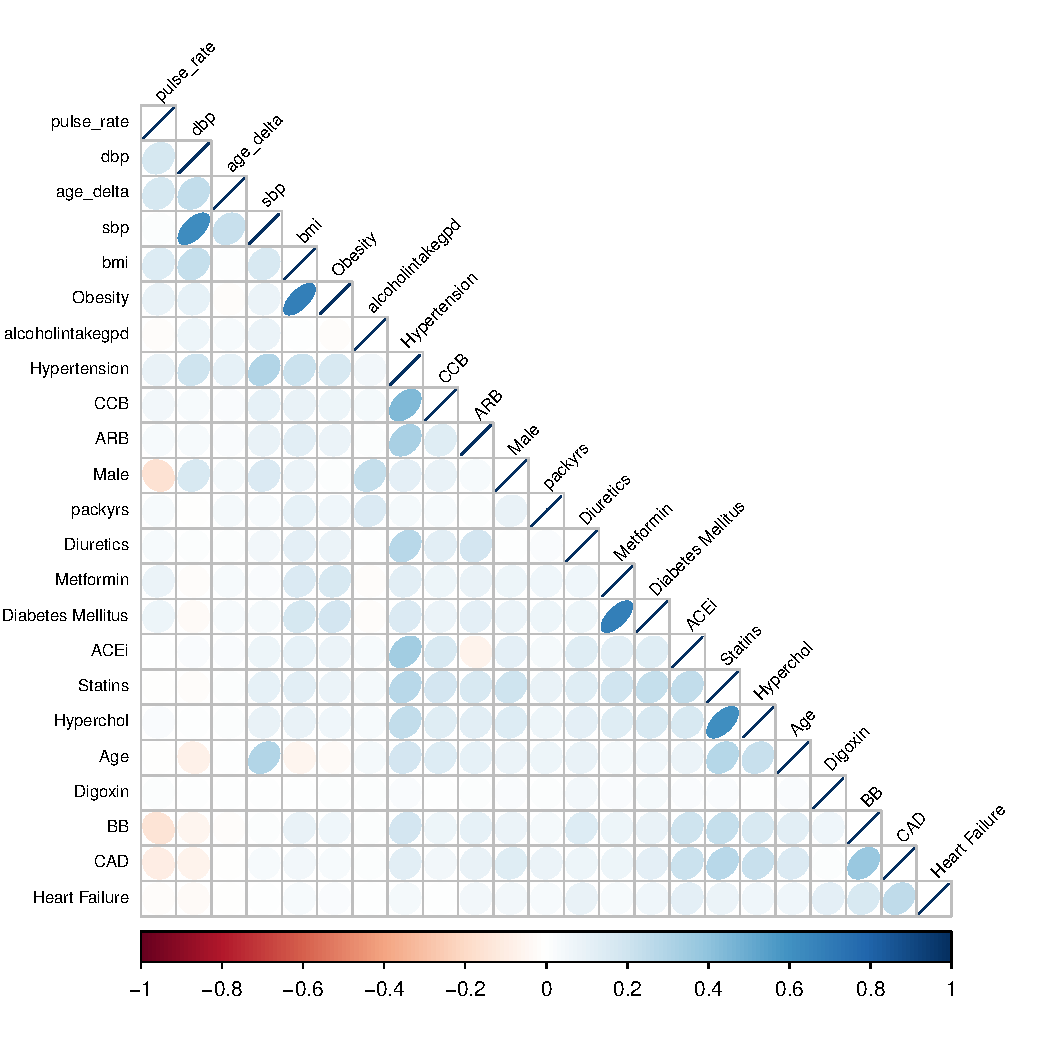
\includegraphics{../results/report_files/figure-latex/feature-corr-plot-1.pdf}

\begin{Shaded}
\begin{Highlighting}[]
\NormalTok{corrplot}\SpecialCharTok{::}\FunctionTok{corrplot}\NormalTok{( M,}
                   \AttributeTok{method=}\StringTok{"ellipse"}\NormalTok{,}
                   \AttributeTok{type=}\StringTok{"lower"}\NormalTok{,}
                   \AttributeTok{na.label=}\StringTok{\textquotesingle{}{-}\textquotesingle{}}\NormalTok{, }
                   \AttributeTok{tl.cex =} \FloatTok{0.7}\NormalTok{, }
                   \AttributeTok{order=}\StringTok{"hclust"}\NormalTok{,}
                   \AttributeTok{tl.col=}\StringTok{"black"}\NormalTok{,}
                   \AttributeTok{tl.srt=}\DecValTok{45}\NormalTok{,}
                   \AttributeTok{number.cex =} \FloatTok{0.3}\NormalTok{) }
\end{Highlighting}
\end{Shaded}

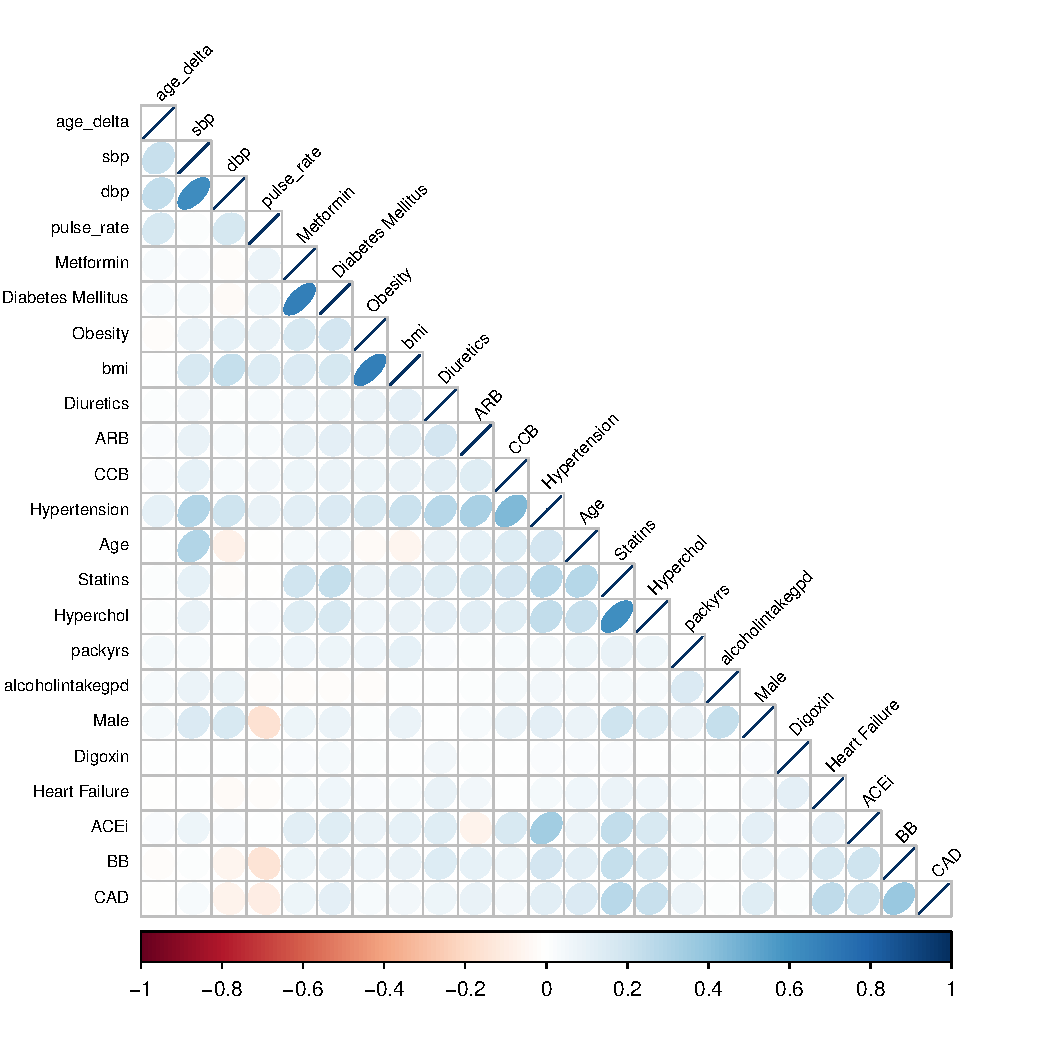
\includegraphics{../results/report_files/figure-latex/feature-corr-plot-hclust-1.pdf}

\hypertarget{medication-effect-overview}{%
\subsection{Medication-Effect
Overview}\label{medication-effect-overview}}

\hypertarget{forest-plot}{%
\subsubsection{Forest plot}\label{forest-plot}}

\begin{Shaded}
\begin{Highlighting}[]
\NormalTok{(fits.df  }\SpecialCharTok{\%\textgreater{}\%} 
  \FunctionTok{filter}\NormalTok{(term}\SpecialCharTok{==}\StringTok{"PriorMed"}\NormalTok{) }\SpecialCharTok{\%\textgreater{}\%} 
  \FunctionTok{mutate}\NormalTok{(}\AttributeTok{Adjustment=}\FunctionTok{if\_else}\NormalTok{(AdditionalMarkers}\SpecialCharTok{==}\ConstantTok{TRUE}\NormalTok{, }\StringTok{"With SBP/DBP/HR"}\NormalTok{, }\StringTok{"Without SBP/DBP/HR"}\NormalTok{)) }\SpecialCharTok{\%\textgreater{}\%} 
  \FunctionTok{mutate}\NormalTok{(}\AttributeTok{Adjustment=}\FunctionTok{factor}\NormalTok{(Adjustment, }\AttributeTok{levels=}\FunctionTok{c}\NormalTok{(}\StringTok{"Without SBP/DBP/HR"}\NormalTok{,}\StringTok{"With SBP/DBP/HR"}\NormalTok{), }\AttributeTok{ordered=}\ConstantTok{TRUE}\NormalTok{)) }\SpecialCharTok{\%\textgreater{}\%} 
  \FunctionTok{ggplot}\NormalTok{(}\FunctionTok{aes}\NormalTok{(}\AttributeTok{x=}\NormalTok{Drug, }\AttributeTok{y=}\NormalTok{estimate, }\AttributeTok{ymin=}\NormalTok{conf.low, }\AttributeTok{ymax=}\NormalTok{conf.high, }\AttributeTok{color=}\NormalTok{Adjustment))}\SpecialCharTok{+}
  \FunctionTok{geom\_point}\NormalTok{( }\AttributeTok{position=}\FunctionTok{position\_dodge}\NormalTok{(}\AttributeTok{width=}\FloatTok{0.3}\NormalTok{))}\SpecialCharTok{+}
  \FunctionTok{geom\_linerange}\NormalTok{( }\AttributeTok{position=}\FunctionTok{position\_dodge}\NormalTok{(}\AttributeTok{width=}\FloatTok{0.3}\NormalTok{))}\SpecialCharTok{+}
  \FunctionTok{coord\_flip}\NormalTok{()}\SpecialCharTok{+}
  \FunctionTok{xlab}\NormalTok{(}\StringTok{"Drug"}\NormalTok{)}\SpecialCharTok{+}
  \FunctionTok{ylab}\NormalTok{(}\StringTok{"Coefficient"}\NormalTok{)}\SpecialCharTok{+}
  \FunctionTok{geom\_hline}\NormalTok{(}\AttributeTok{yintercept=}\DecValTok{0}\NormalTok{, }\AttributeTok{alpha=}\FloatTok{0.5}\NormalTok{, }\AttributeTok{linetype=}\StringTok{"dashed"}\NormalTok{)}\SpecialCharTok{+}
  \FunctionTok{scale\_color\_manual}\NormalTok{(}\AttributeTok{values =} \FunctionTok{c}\NormalTok{(}\StringTok{"Without SBP/DBP/HR"} \OtherTok{=} \StringTok{"red"}\NormalTok{,}
                                    \StringTok{"With SBP/DBP/HR"} \OtherTok{=} \StringTok{"forestgreen"}
\NormalTok{                                    )) }\OtherTok{{-}\textgreater{}}\NormalTok{ p)}
\end{Highlighting}
\end{Shaded}

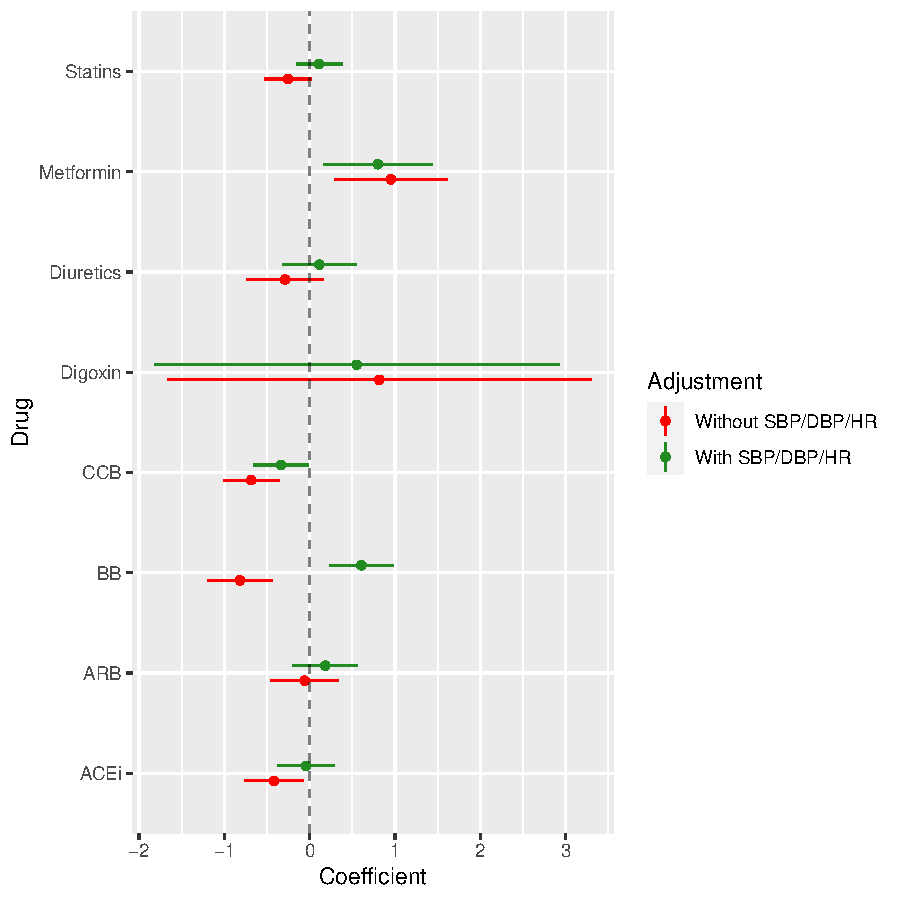
\includegraphics{../results/report_files/figure-latex/med-effect-forest-2-1.pdf}

\begin{Shaded}
\begin{Highlighting}[]
\NormalTok{p}\SpecialCharTok{+}\FunctionTok{geom\_segment}\NormalTok{(}\FunctionTok{aes}\NormalTok{(}\AttributeTok{y =} \FloatTok{0.05}\NormalTok{, }\AttributeTok{x =}\NormalTok{ .}\DecValTok{55}\NormalTok{, }\AttributeTok{yend =} \DecValTok{3}\NormalTok{, }\AttributeTok{xend =}\NormalTok{ .}\DecValTok{55}\NormalTok{),}
                  \AttributeTok{arrow =} \FunctionTok{arrow}\NormalTok{(}\AttributeTok{length =} \FunctionTok{unit}\NormalTok{(}\FloatTok{0.25}\NormalTok{, }\StringTok{"cm"}\NormalTok{)), }\AttributeTok{show.legend=}\ConstantTok{FALSE}\NormalTok{, }\AttributeTok{color=}\StringTok{"black"}\NormalTok{)}\SpecialCharTok{+}
    \FunctionTok{geom\_text}\NormalTok{(}\FunctionTok{aes}\NormalTok{(}\AttributeTok{y =} \FloatTok{1.5}\NormalTok{, }\AttributeTok{x =}\NormalTok{ .}\DecValTok{725}\NormalTok{, }\AttributeTok{label =} \StringTok{"Drug increases cardiac age gap"}\NormalTok{), }\AttributeTok{size=}\DecValTok{3}\NormalTok{, }\AttributeTok{color=}\StringTok{"black"}\NormalTok{) }\SpecialCharTok{+}
\FunctionTok{geom\_segment}\NormalTok{(}\FunctionTok{aes}\NormalTok{(}\AttributeTok{y =} \SpecialCharTok{{-}}\FloatTok{0.05}\NormalTok{, }\AttributeTok{x =}\NormalTok{ .}\DecValTok{55}\NormalTok{, }\AttributeTok{yend =} \SpecialCharTok{{-}}\DecValTok{3}\NormalTok{, }\AttributeTok{xend =}\NormalTok{ .}\DecValTok{55}\NormalTok{),}
                  \AttributeTok{arrow =} \FunctionTok{arrow}\NormalTok{(}\AttributeTok{length =} \FunctionTok{unit}\NormalTok{(}\FloatTok{0.25}\NormalTok{, }\StringTok{"cm"}\NormalTok{)), }\AttributeTok{show.legend=}\ConstantTok{FALSE}\NormalTok{, }\AttributeTok{color=}\StringTok{"black"}\NormalTok{)}\SpecialCharTok{+}
    \FunctionTok{geom\_text}\NormalTok{(}\FunctionTok{aes}\NormalTok{(}\AttributeTok{y =} \SpecialCharTok{{-}}\FloatTok{1.5}\NormalTok{, }\AttributeTok{x =}\NormalTok{ .}\DecValTok{725}\NormalTok{, }\AttributeTok{label =} \StringTok{"Drug decreases cardiac age gap"}\NormalTok{), }\AttributeTok{size=}\DecValTok{3}\NormalTok{, }\AttributeTok{color=}\StringTok{"black"}\NormalTok{)}
\end{Highlighting}
\end{Shaded}

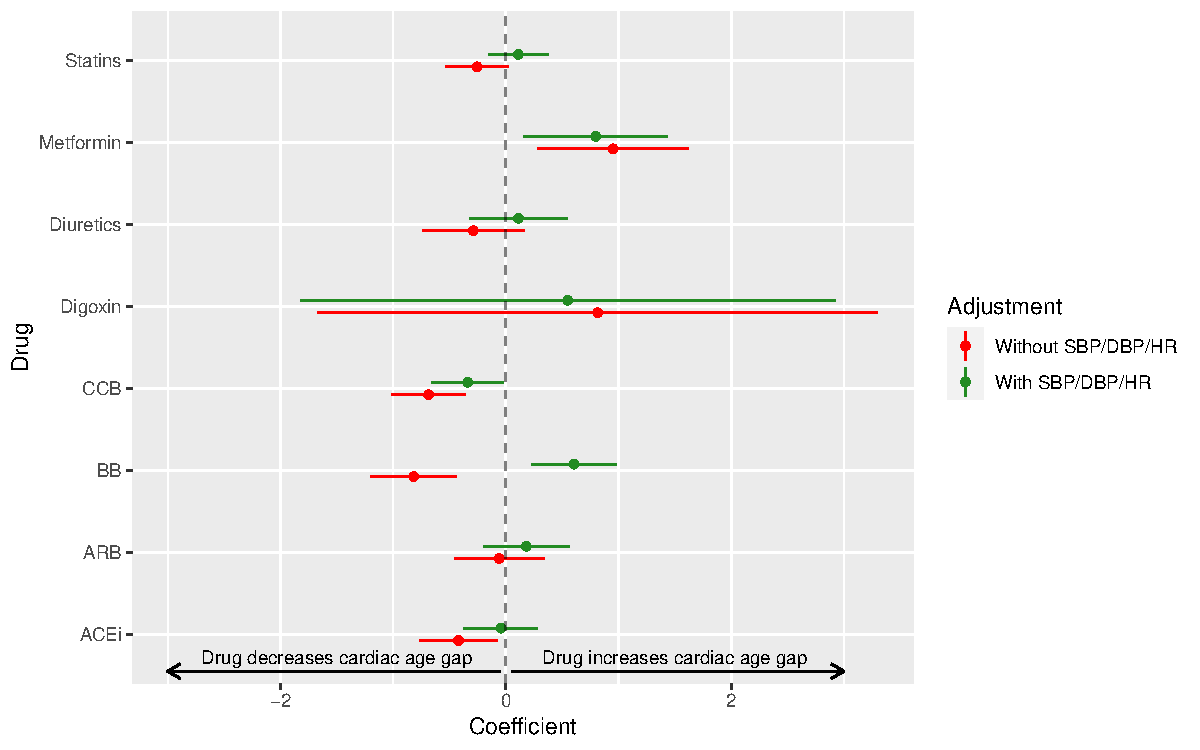
\includegraphics{../results/report_files/figure-latex/med-effect-forest-2-with-arrows-1.pdf}

\begin{Shaded}
\begin{Highlighting}[]
\NormalTok{(fits.df  }\SpecialCharTok{\%\textgreater{}\%} 
  \FunctionTok{filter}\NormalTok{(term}\SpecialCharTok{==}\StringTok{"PriorMed"}\NormalTok{) }\SpecialCharTok{\%\textgreater{}\%} 
  \FunctionTok{filter}\NormalTok{(AdditionalMarkers}\SpecialCharTok{==}\ConstantTok{TRUE}\NormalTok{) }\SpecialCharTok{\%\textgreater{}\%} 
  \FunctionTok{ggplot}\NormalTok{(}\FunctionTok{aes}\NormalTok{(}\AttributeTok{x=}\NormalTok{Drug, }\AttributeTok{y=}\NormalTok{estimate, }\AttributeTok{ymin=}\NormalTok{conf.low, }\AttributeTok{ymax=}\NormalTok{conf.high))}\SpecialCharTok{+}
  \FunctionTok{geom\_point}\NormalTok{( )}\SpecialCharTok{+}
  \FunctionTok{geom\_linerange}\NormalTok{()}\SpecialCharTok{+}
  \FunctionTok{coord\_flip}\NormalTok{()}\SpecialCharTok{+}
  \FunctionTok{xlab}\NormalTok{(}\StringTok{"Drug"}\NormalTok{)}\SpecialCharTok{+}
  \FunctionTok{ylab}\NormalTok{(}\StringTok{"Coefficient"}\NormalTok{)}\SpecialCharTok{+}
  \FunctionTok{geom\_hline}\NormalTok{(}\AttributeTok{yintercept=}\DecValTok{0}\NormalTok{, }\AttributeTok{alpha=}\FloatTok{0.5}\NormalTok{, }\AttributeTok{linetype=}\StringTok{"dashed"}\NormalTok{) }\OtherTok{{-}\textgreater{}}\NormalTok{ p)}
\end{Highlighting}
\end{Shaded}

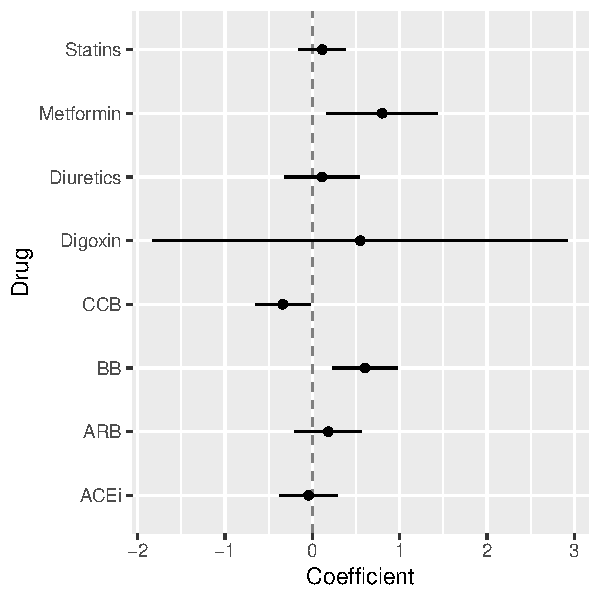
\includegraphics{../results/report_files/figure-latex/med-effect-forest-1.pdf}

\begin{Shaded}
\begin{Highlighting}[]
\NormalTok{fits.df  }\SpecialCharTok{\%\textgreater{}\%} 
  \FunctionTok{filter}\NormalTok{(term}\SpecialCharTok{==}\StringTok{"PriorMed"}\NormalTok{) }\SpecialCharTok{\%\textgreater{}\%} 
  \FunctionTok{filter}\NormalTok{(AdditionalMarkers}\SpecialCharTok{==}\ConstantTok{TRUE}\NormalTok{) }\SpecialCharTok{\%\textgreater{}\%} 
  \FunctionTok{mutate}\NormalTok{(}\AttributeTok{n=}\FunctionTok{round}\NormalTok{(fracPriorMed}\SpecialCharTok{*}\NormalTok{nobs)) }\OtherTok{{-}\textgreater{}}
\NormalTok{  phewas\_results}

\NormalTok{plot\_data }\OtherTok{\textless{}{-}}\NormalTok{ phewas\_results }\SpecialCharTok{\%\textgreater{}\%}
\NormalTok{    dplyr}\SpecialCharTok{::}\FunctionTok{select}\NormalTok{(Drug, p.value, estimate, conf.high, conf.low, n) }\SpecialCharTok{\%\textgreater{}\%}
\NormalTok{    dplyr}\SpecialCharTok{::}\FunctionTok{mutate}\NormalTok{(}\AttributeTok{p.value.str=}\FunctionTok{sprintf}\NormalTok{(}\StringTok{"\%.3f"}\NormalTok{, p.value), }\AttributeTok{beta.str=}\FunctionTok{sprintf}\NormalTok{(}\StringTok{"\%.2f"}\NormalTok{, estimate))}

\NormalTok{  parm }\OtherTok{\textless{}{-}}\NormalTok{ plot\_data }\SpecialCharTok{\%\textgreater{}\%}\NormalTok{ dplyr}\SpecialCharTok{::}\FunctionTok{mutate}\NormalTok{(}\AttributeTok{mean=}\NormalTok{estimate,}\AttributeTok{lower=}\NormalTok{conf.low,}\AttributeTok{upper=}\NormalTok{conf.high) }\SpecialCharTok{\%\textgreater{}\%}
\NormalTok{    dplyr}\SpecialCharTok{::}\FunctionTok{select}\NormalTok{(mean, lower, upper)}
\NormalTok{  parm }\OtherTok{\textless{}{-}} \FunctionTok{rbind}\NormalTok{(}\FunctionTok{rep}\NormalTok{(}\ConstantTok{NA}\NormalTok{,}\DecValTok{3}\NormalTok{), parm)}

\NormalTok{  labeltext }\OtherTok{\textless{}{-}}\NormalTok{ plot\_data }\SpecialCharTok{\%\textgreater{}\%}\NormalTok{ dplyr}\SpecialCharTok{::}\FunctionTok{select}\NormalTok{(Drug, n, beta.str, p.value.str)}
  \ControlFlowTok{if}\NormalTok{ (}\FunctionTok{nrow}\NormalTok{(labeltext)}\SpecialCharTok{\textgreater{}}\DecValTok{1}\NormalTok{) \{}
\NormalTok{    labeltext }\OtherTok{\textless{}{-}} \FunctionTok{as.matrix}\NormalTok{(}\FunctionTok{sapply}\NormalTok{(labeltext, as.character))}
\NormalTok{  \}}
\NormalTok{  labeltext }\OtherTok{\textless{}{-}} \FunctionTok{rbind}\NormalTok{(}\FunctionTok{c}\NormalTok{(}\StringTok{\textquotesingle{}Drug\textquotesingle{}}\NormalTok{,}\StringTok{\textquotesingle{}N\textquotesingle{}}\NormalTok{, }\StringTok{\textquotesingle{}Coefficient\textquotesingle{}}\NormalTok{, }\StringTok{\textquotesingle{}P{-}Value\textquotesingle{}}\NormalTok{), labeltext)}
\end{Highlighting}
\end{Shaded}

\begin{Shaded}
\begin{Highlighting}[]
\NormalTok{fig\_width }\OtherTok{\textless{}{-}} \DecValTok{8}
\NormalTok{forestplot}\SpecialCharTok{::}\FunctionTok{forestplot}\NormalTok{(}\AttributeTok{labeltext=}\NormalTok{labeltext, }
\NormalTok{                       parm, }
                       \AttributeTok{zero=}\DecValTok{0}\NormalTok{, }
                       \AttributeTok{xlab=}\StringTok{\textquotesingle{}Coefficient\textquotesingle{}}\NormalTok{,}
                       \AttributeTok{title =} \StringTok{"Medication Effects"}\NormalTok{, }
                       \AttributeTok{is.summary=}\FunctionTok{c}\NormalTok{(}\ConstantTok{TRUE}\NormalTok{, }\FunctionTok{rep}\NormalTok{(}\ConstantTok{FALSE}\NormalTok{, }\FunctionTok{nrow}\NormalTok{(plot\_data))) ,}
                       \AttributeTok{txt\_gp=}\NormalTok{forestplot}\SpecialCharTok{::}\FunctionTok{fpTxtGp}\NormalTok{(}\AttributeTok{ticks=}\FunctionTok{gpar}\NormalTok{(}\AttributeTok{cex=}\FloatTok{1.2}\NormalTok{),}\AttributeTok{xlab=}\FunctionTok{gpar}\NormalTok{(}\AttributeTok{cex=}\FloatTok{1.5}\NormalTok{), }\AttributeTok{title =} \FunctionTok{gpar}\NormalTok{(}\AttributeTok{cex=}\FloatTok{2.0}\NormalTok{), }\AttributeTok{cex=}\FloatTok{1.2}\NormalTok{), }
                       \AttributeTok{graph.pos =} \DecValTok{4}\NormalTok{,}
                       \AttributeTok{graphwidth =}\NormalTok{ grid}\SpecialCharTok{::}\FunctionTok{unit}\NormalTok{(fig\_width,}\StringTok{"cm"}\NormalTok{), }
                       \AttributeTok{lwd.zero=}\DecValTok{3}\NormalTok{, }
                       \AttributeTok{lwd.ci=}\DecValTok{3}\NormalTok{)}
\end{Highlighting}
\end{Shaded}

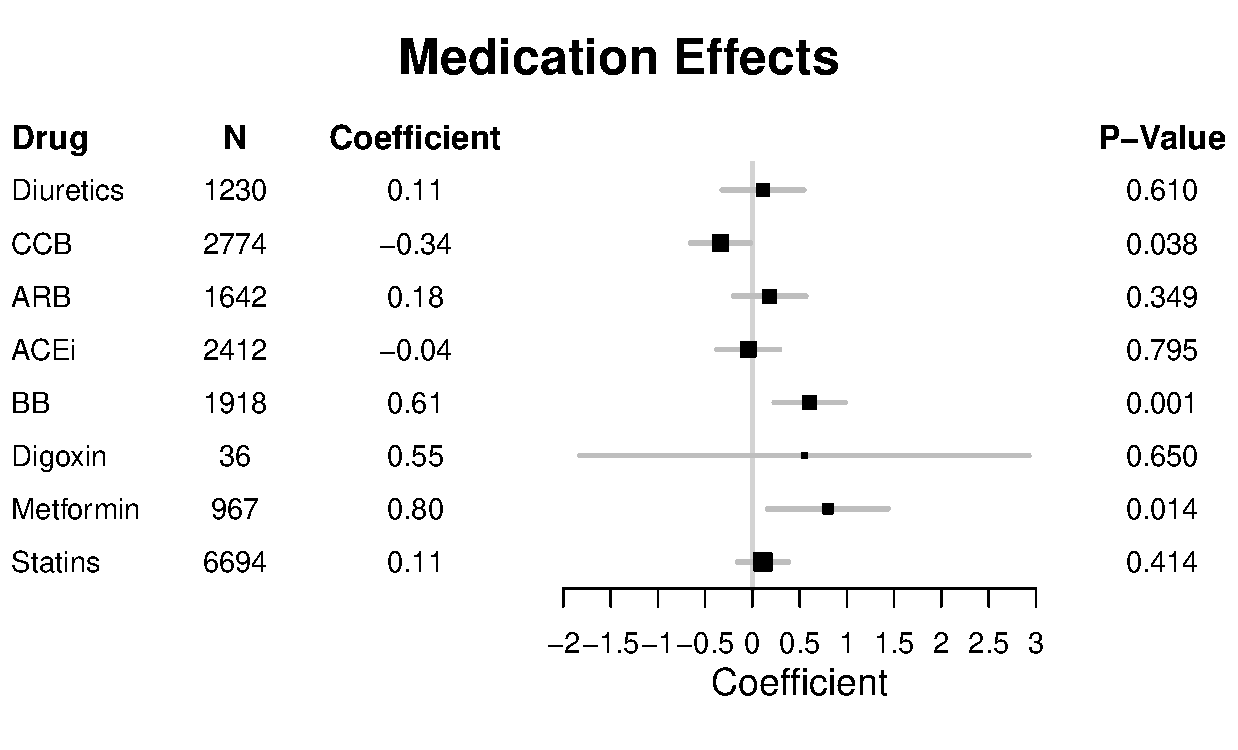
\includegraphics{../results/report_files/figure-latex/med-effect-forest-ukbrlib-2-1.pdf}

\hypertarget{table}{%
\subsubsection{Table}\label{table}}

\begin{Shaded}
\begin{Highlighting}[]
\NormalTok{fits.df  }\SpecialCharTok{\%\textgreater{}\%} 
  \FunctionTok{filter}\NormalTok{(term}\SpecialCharTok{==}\StringTok{"PriorMed"}\NormalTok{) }\SpecialCharTok{\%\textgreater{}\%} 
  \FunctionTok{mutate}\NormalTok{(}\AttributeTok{Adjustment=}\FunctionTok{if\_else}\NormalTok{(AdditionalMarkers}\SpecialCharTok{==}\ConstantTok{TRUE}\NormalTok{, }\StringTok{"With SBP/DBP/HR"}\NormalTok{, }\StringTok{"Without SBP/DBP/HR"}\NormalTok{)) }\SpecialCharTok{\%\textgreater{}\%} 
  \FunctionTok{mutate}\NormalTok{(}\AttributeTok{Adjustment=}\FunctionTok{factor}\NormalTok{(Adjustment, }\AttributeTok{levels=}\FunctionTok{c}\NormalTok{(}\StringTok{"Without SBP/DBP/HR"}\NormalTok{,}\StringTok{"With SBP/DBP/HR"}\NormalTok{), }\AttributeTok{ordered=}\ConstantTok{TRUE}\NormalTok{)) }\SpecialCharTok{\%\textgreater{}\%} 
  \FunctionTok{transmute}\NormalTok{(Drug,Adjustment, estimate, std.error, statistic, p.value, conf.low, conf.high) }\SpecialCharTok{\%\textgreater{}\%} 
  \FunctionTok{mutate}\NormalTok{(}\FunctionTok{across}\NormalTok{(}\AttributeTok{.cols=}\NormalTok{estimate}\SpecialCharTok{:}\NormalTok{conf.high, }\SpecialCharTok{\textasciitilde{}}\FunctionTok{round}\NormalTok{(.,}\DecValTok{2}\NormalTok{)))}\OtherTok{{-}\textgreater{}}\NormalTok{table1}
\end{Highlighting}
\end{Shaded}

\begin{Shaded}
\begin{Highlighting}[]
\NormalTok{table1 }\SpecialCharTok{\%\textgreater{}\%} 
  \FunctionTok{kbl}\NormalTok{(}\AttributeTok{caption =} \StringTok{"Table S1: Coefficients of self{-}reported drugs"}\NormalTok{) }\SpecialCharTok{\%\textgreater{}\%}
  \FunctionTok{kable\_classic}\NormalTok{(}\AttributeTok{full\_width =}\NormalTok{ F, }\AttributeTok{html\_font =} \StringTok{"Cambria"}\NormalTok{)}
\end{Highlighting}
\end{Shaded}

\begin{table}

\caption{\label{tab:med-effect-table-2}Table S1: Coefficients of self-reported drugs}
\centering
\begin{tabular}[t]{l|l|r|r|r|r|r|r}
\hline
Drug & Adjustment & estimate & std.error & statistic & p.value & conf.low & conf.high\\
\hline
Diuretics & With SBP/DBP/HR & 0.11 & 0.22 & 0.51 & 0.61 & -0.32 & 0.55\\
\hline
Diuretics & Without SBP/DBP/HR & -0.29 & 0.23 & -1.25 & 0.21 & -0.74 & 0.16\\
\hline
CCB & With SBP/DBP/HR & -0.34 & 0.16 & -2.08 & 0.04 & -0.66 & -0.02\\
\hline
CCB & Without SBP/DBP/HR & -0.69 & 0.17 & -4.05 & 0.00 & -1.02 & -0.35\\
\hline
ARB & With SBP/DBP/HR & 0.18 & 0.20 & 0.94 & 0.35 & -0.20 & 0.57\\
\hline
ARB & Without SBP/DBP/HR & -0.06 & 0.20 & -0.29 & 0.77 & -0.46 & 0.34\\
\hline
ACEi & With SBP/DBP/HR & -0.04 & 0.17 & -0.26 & 0.79 & -0.37 & 0.29\\
\hline
ACEi & Without SBP/DBP/HR & -0.42 & 0.18 & -2.39 & 0.02 & -0.76 & -0.08\\
\hline
BB & With SBP/DBP/HR & 0.61 & 0.19 & 3.18 & 0.00 & 0.23 & 0.98\\
\hline
BB & Without SBP/DBP/HR & -0.82 & 0.20 & -4.17 & 0.00 & -1.20 & -0.43\\
\hline
Digoxin & With SBP/DBP/HR & 0.55 & 1.21 & 0.45 & 0.65 & -1.83 & 2.92\\
\hline
Digoxin & Without SBP/DBP/HR & 0.82 & 1.27 & 0.64 & 0.52 & -1.67 & 3.30\\
\hline
Metformin & With SBP/DBP/HR & 0.80 & 0.33 & 2.46 & 0.01 & 0.16 & 1.44\\
\hline
Metformin & Without SBP/DBP/HR & 0.95 & 0.34 & 2.80 & 0.01 & 0.29 & 1.62\\
\hline
Statins & With SBP/DBP/HR & 0.11 & 0.14 & 0.82 & 0.41 & -0.16 & 0.38\\
\hline
Statins & Without SBP/DBP/HR & -0.25 & 0.14 & -1.78 & 0.07 & -0.53 & 0.03\\
\hline
\end{tabular}
\end{table}

\begin{Shaded}
\begin{Highlighting}[]
\NormalTok{fits.df  }\SpecialCharTok{\%\textgreater{}\%} 
  \FunctionTok{filter}\NormalTok{(term}\SpecialCharTok{==}\StringTok{"PriorMed"}\NormalTok{) }\SpecialCharTok{\%\textgreater{}\%} 
  \FunctionTok{filter}\NormalTok{(AdditionalMarkers}\SpecialCharTok{==}\ConstantTok{TRUE}\NormalTok{) }\SpecialCharTok{\%\textgreater{}\%} 
  \FunctionTok{select}\NormalTok{(}\SpecialCharTok{{-}}\NormalTok{AdditionalMarkers) }\SpecialCharTok{\%\textgreater{}\%} 
  \FunctionTok{transmute}\NormalTok{(Drug, estimate, std.error, statistic, p.value, conf.low, conf.high) }\SpecialCharTok{\%\textgreater{}\%} 
  \FunctionTok{mutate}\NormalTok{(}\FunctionTok{across}\NormalTok{(}\AttributeTok{.cols=}\NormalTok{estimate}\SpecialCharTok{:}\NormalTok{conf.high, }\SpecialCharTok{\textasciitilde{}}\FunctionTok{round}\NormalTok{(.,}\DecValTok{2}\NormalTok{))) }\OtherTok{{-}\textgreater{}}\NormalTok{ table2}
\end{Highlighting}
\end{Shaded}

\begin{Shaded}
\begin{Highlighting}[]
\NormalTok{table2 }\SpecialCharTok{\%\textgreater{}\%} 
  \FunctionTok{kbl}\NormalTok{(}\AttributeTok{caption =} \StringTok{"Table 1: Coefficients of self{-}reported drugs"}\NormalTok{) }\SpecialCharTok{\%\textgreater{}\%}
  \FunctionTok{kable\_classic}\NormalTok{(}\AttributeTok{full\_width =}\NormalTok{ F, }\AttributeTok{html\_font =} \StringTok{"Cambria"}\NormalTok{)}
\end{Highlighting}
\end{Shaded}

\begin{table}

\caption{\label{tab:med-effect-table}Table 1: Coefficients of self-reported drugs}
\centering
\begin{tabular}[t]{l|r|r|r|r|r|r}
\hline
Drug & estimate & std.error & statistic & p.value & conf.low & conf.high\\
\hline
Diuretics & 0.11 & 0.22 & 0.51 & 0.61 & -0.32 & 0.55\\
\hline
CCB & -0.34 & 0.16 & -2.08 & 0.04 & -0.66 & -0.02\\
\hline
ARB & 0.18 & 0.20 & 0.94 & 0.35 & -0.20 & 0.57\\
\hline
ACEi & -0.04 & 0.17 & -0.26 & 0.79 & -0.37 & 0.29\\
\hline
BB & 0.61 & 0.19 & 3.18 & 0.00 & 0.23 & 0.98\\
\hline
Digoxin & 0.55 & 1.21 & 0.45 & 0.65 & -1.83 & 2.92\\
\hline
Metformin & 0.80 & 0.33 & 2.46 & 0.01 & 0.16 & 1.44\\
\hline
Statins & 0.11 & 0.14 & 0.82 & 0.41 & -0.16 & 0.38\\
\hline
\end{tabular}
\end{table}

\hypertarget{statins}{%
\subsection{Statins}\label{statins}}

\begin{Shaded}
\begin{Highlighting}[]
\NormalTok{statin.df }\OtherTok{\textless{}{-}}\NormalTok{ dfs }\SpecialCharTok{\%\textgreater{}\%} 
  \FunctionTok{filter}\NormalTok{(Drug}\SpecialCharTok{==}\StringTok{"Statins"}\NormalTok{) }\SpecialCharTok{\%\textgreater{}\%} 
  \FunctionTok{select}\NormalTok{(}\SpecialCharTok{{-}}\NormalTok{Drug)}
\end{Highlighting}
\end{Shaded}

\begin{Shaded}
\begin{Highlighting}[]
\NormalTok{statin.fits.df }\OtherTok{\textless{}{-}}\NormalTok{ fits.df }\SpecialCharTok{\%\textgreater{}\%} 
  \FunctionTok{filter}\NormalTok{(Drug}\SpecialCharTok{==}\StringTok{"Statins"}\NormalTok{)}
\end{Highlighting}
\end{Shaded}

\begin{Shaded}
\begin{Highlighting}[]
\FunctionTok{get\_pretty\_fit\_table}\NormalTok{(statin.fits.df, }\StringTok{"Statins"}\NormalTok{)}
\end{Highlighting}
\end{Shaded}

\begin{table}

\caption{\label{tab:statin-fit-table}Statins: Coefficients from linear models}
\centering
\begin{tabular}[t]{l|r|r|r|r|r|r|l}
\hline
term & estimate & std.error & statistic & p.value & conf.low & conf.high & Adjustment\\
\hline
(Intercept) & -20.526 & 0.517 & -39.703 & 0.000 & -21.539 & -19.512 & With SBP/DBP/HR\\
\hline
(Intercept) & -0.876 & 0.359 & -2.437 & 0.015 & -1.580 & -0.171 & Without SBP/DBP/HR\\
\hline
`Diabetes Mellitus`TRUE & 0.645 & 0.178 & 3.628 & 0.000 & 0.297 & 0.994 & With SBP/DBP/HR\\
\hline
`Diabetes Mellitus`TRUE & 0.649 & 0.185 & 3.510 & 0.000 & 0.287 & 1.012 & Without SBP/DBP/HR\\
\hline
`Heart Failure`TRUE & 0.107 & 0.370 & 0.288 & 0.773 & -0.619 & 0.832 & With SBP/DBP/HR\\
\hline
`Heart Failure`TRUE & -0.125 & 0.387 & -0.323 & 0.746 & -0.885 & 0.634 & Without SBP/DBP/HR\\
\hline
alcoholintakegpd & 0.001 & 0.003 & 0.328 & 0.743 & -0.004 & 0.006 & With SBP/DBP/HR\\
\hline
alcoholintakegpd & 0.006 & 0.003 & 2.325 & 0.020 & 0.001 & 0.011 & Without SBP/DBP/HR\\
\hline
bmi & -0.147 & 0.014 & -10.553 & 0.000 & -0.175 & -0.120 & With SBP/DBP/HR\\
\hline
bmi & 0.000 & 0.014 & -0.002 & 0.999 & -0.028 & 0.028 & Without SBP/DBP/HR\\
\hline
CADTRUE & 0.438 & 0.178 & 2.461 & 0.014 & 0.089 & 0.786 & With SBP/DBP/HR\\
\hline
CADTRUE & -0.440 & 0.185 & -2.381 & 0.017 & -0.803 & -0.078 & Without SBP/DBP/HR\\
\hline
dbp & 0.087 & 0.006 & 14.002 & 0.000 & 0.075 & 0.100 & With SBP/DBP/HR\\
\hline
HypercholTRUE & -0.198 & 0.132 & -1.497 & 0.134 & -0.458 & 0.061 & With SBP/DBP/HR\\
\hline
HypercholTRUE & -0.095 & 0.138 & -0.684 & 0.494 & -0.366 & 0.177 & Without SBP/DBP/HR\\
\hline
HypertensionTRUE & 0.646 & 0.103 & 6.298 & 0.000 & 0.445 & 0.846 & With SBP/DBP/HR\\
\hline
HypertensionTRUE & 1.838 & 0.104 & 17.683 & 0.000 & 1.634 & 2.042 & Without SBP/DBP/HR\\
\hline
ObesityTRUE & -0.255 & 0.148 & -1.722 & 0.085 & -0.546 & 0.035 & With SBP/DBP/HR\\
\hline
ObesityTRUE & -0.741 & 0.155 & -4.786 & 0.000 & -1.044 & -0.437 & Without SBP/DBP/HR\\
\hline
packyrs & 0.023 & 0.004 & 6.029 & 0.000 & 0.015 & 0.030 & With SBP/DBP/HR\\
\hline
packyrs & 0.022 & 0.004 & 5.499 & 0.000 & 0.014 & 0.030 & Without SBP/DBP/HR\\
\hline
poly(Age, 2)1 & -69.744 & 8.444 & -8.260 & 0.000 & -86.294 & -53.194 & With SBP/DBP/HR\\
\hline
poly(Age, 2)1 & -22.395 & 8.031 & -2.788 & 0.005 & -38.137 & -6.653 & Without SBP/DBP/HR\\
\hline
poly(Age, 2)2 & -106.586 & 7.248 & -14.705 & 0.000 & -120.793 & -92.378 & With SBP/DBP/HR\\
\hline
poly(Age, 2)2 & -112.960 & 7.565 & -14.932 & 0.000 & -127.787 & -98.132 & Without SBP/DBP/HR\\
\hline
PriorMed & 0.112 & 0.137 & 0.818 & 0.414 & -0.156 & 0.380 & With SBP/DBP/HR\\
\hline
PriorMed & -0.254 & 0.143 & -1.781 & 0.075 & -0.534 & 0.026 & Without SBP/DBP/HR\\
\hline
pulse\_rate & 0.110 & 0.004 & 27.855 & 0.000 & 0.103 & 0.118 & With SBP/DBP/HR\\
\hline
sbp & 0.067 & 0.003 & 19.643 & 0.000 & 0.061 & 0.074 & With SBP/DBP/HR\\
\hline
SexMale & 0.442 & 0.095 & 4.648 & 0.000 & 0.256 & 0.629 & With SBP/DBP/HR\\
\hline
SexMale & 0.540 & 0.096 & 5.593 & 0.000 & 0.351 & 0.729 & Without SBP/DBP/HR\\
\hline
\end{tabular}
\end{table}

\begin{Shaded}
\begin{Highlighting}[]
\FunctionTok{get\_pretty\_fit\_forest\_plot}\NormalTok{(statin.fits.df) }\OtherTok{{-}\textgreater{}}\NormalTok{p}
\NormalTok{p}
\end{Highlighting}
\end{Shaded}

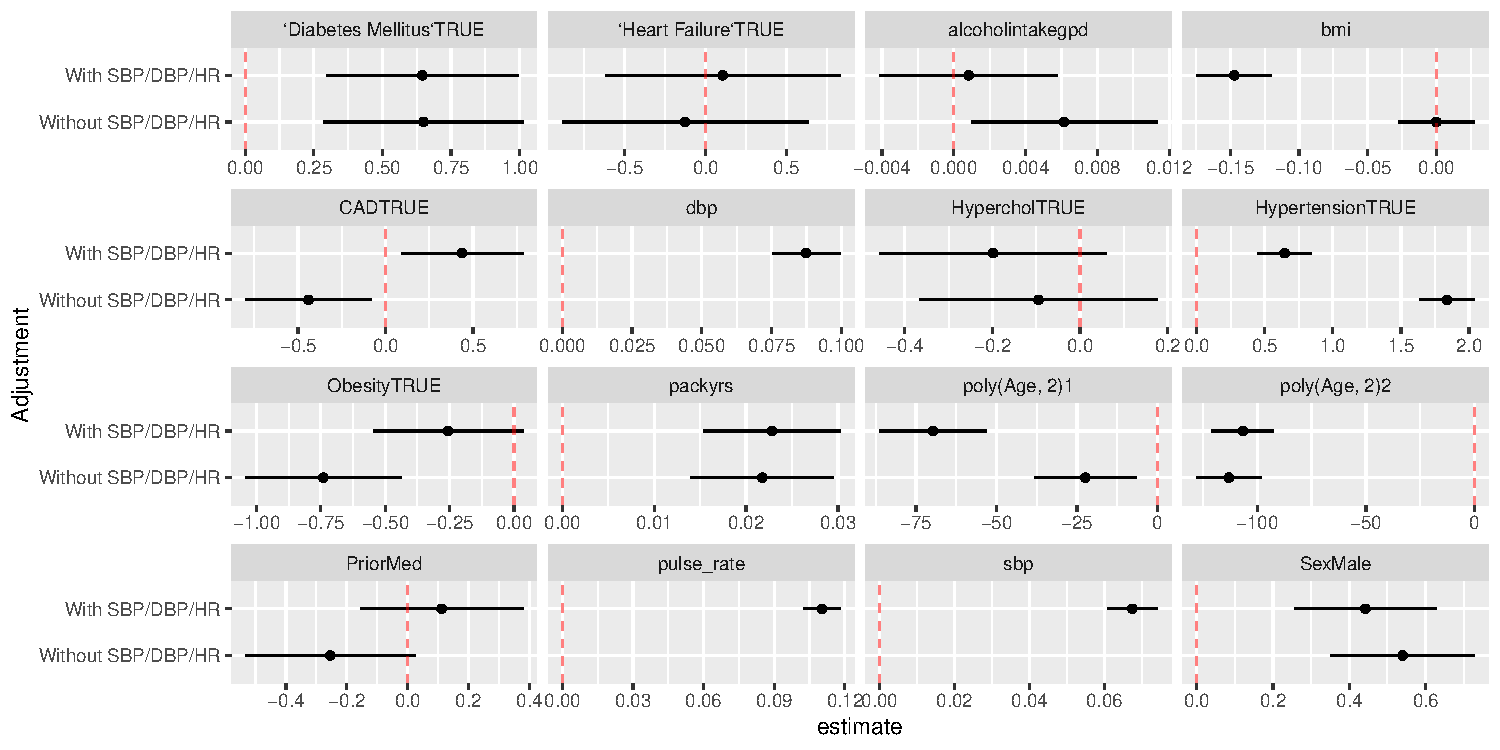
\includegraphics{../results/report_files/figure-latex/statin-fit-forest-1.pdf}

\begin{Shaded}
\begin{Highlighting}[]
\NormalTok{statin.fits.df }\SpecialCharTok{\%\textgreater{}\%} 
\NormalTok{  get\_fit\_glance}
\end{Highlighting}
\end{Shaded}

\begin{verbatim}
## # A tibble: 2 x 5
##   AdditionalMarkers     N fracPriorMed adj.r.squared r.squared
##   <lgl>             <dbl>        <dbl>         <dbl>     <dbl>
## 1 FALSE             27546        0.243         0.024     0.024
## 2 TRUE              27546        0.243         0.108     0.109
\end{verbatim}

\begin{Shaded}
\begin{Highlighting}[]
\FunctionTok{generate\_table.self.reported}\NormalTok{(statin.df, }\StringTok{"Statins"}\NormalTok{)}
\end{Highlighting}
\end{Shaded}

\begin{verbatim}
## Table printed with `knitr::kable()`, not {gt}. Learn why at
## https://www.danieldsjoberg.com/gtsummary/articles/rmarkdown.html
## To suppress this message, include `message = FALSE` in code chunk header.
\end{verbatim}

\begin{tabular}{l|c|c|c}
\hline
**Characteristic** & **No Statins**, N = 20,852 & **Statins**, N = 6,694 & **p-value**\\
\hline
Cardiac Age gap & 0.0 (-5.5, 5.3) & 0.6 (-4.6, 5.3) & <0.001\\
\hline
Sex &  &  & <0.001\\
\hline
Female & 11,672 (56\%) & 2,165 (32\%) & \\
\hline
Male & 9,180 (44\%) & 4,529 (68\%) & \\
\hline
Age & 63 (57, 68) & 69 (64, 72) & <0.001\\
\hline
Packs year of smoking & 0 (0, 1) & 0 (0, 8) & <0.001\\
\hline
Alcohol is g/day consumed & 3 (0, 14) & 4 (0, 18) & <0.001\\
\hline
Hypertension & 5,419 (26\%) & 3,779 (56\%) & <0.001\\
\hline
Obesity & 3,889 (19\%) & 1,786 (27\%) & <0.001\\
\hline
Diabetes Mellitus & 770 (3.7\%) & 1,213 (18\%) & <0.001\\
\hline
Coronary Artery Disease & 727 (3.5\%) & 1,381 (21\%) & <0.001\\
\hline
Hypercholesterolemia & 1,711 (8.2\%) & 4,580 (68\%) & <0.001\\
\hline
Heart Failure & 190 (0.9\%) & 222 (3.3\%) & <0.001\\
\hline
dbp & 78 (72, 86) & 78 (72, 85) & 0.12\\
\hline
sbp & 136 (125, 150) & 142 (130, 154) & <0.001\\
\hline
pulse\_rate & 68 (61, 76) & 68 (60, 76) & 0.054\\
\hline
bmi & 25.9 (23.5, 28.9) & 27.3 (24.9, 30.3) & <0.001\\
\hline
\end{tabular}

\begin{Shaded}
\begin{Highlighting}[]
\NormalTok{statin.df }\SpecialCharTok{\%\textgreater{}\%} 
  \FunctionTok{get\_stratified\_age\_gap\_histogram}\NormalTok{(}\StringTok{"Statins"}\NormalTok{)}
\end{Highlighting}
\end{Shaded}

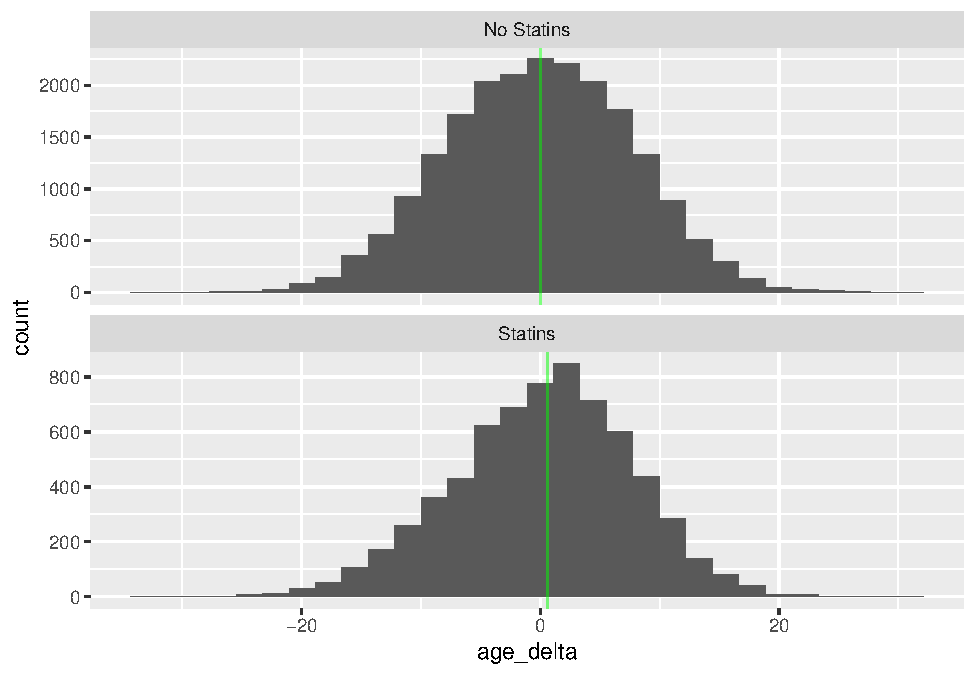
\includegraphics{../results/report_files/figure-latex/statin-age-gap-histograms-1.pdf}

\begin{Shaded}
\begin{Highlighting}[]
\NormalTok{statin.df }\SpecialCharTok{\%\textgreater{}\%} 
  \FunctionTok{get\_stratified\_age\_gap\_quantiles}\NormalTok{(}\StringTok{"Statins"}\NormalTok{)}
\end{Highlighting}
\end{Shaded}

\begin{verbatim}
## # A tibble: 2 x 9
##   PriorMed    `1%` `2.5%` `25%` `50%` `75%` `97.5%` `99%`     N
##   <chr>      <dbl>  <dbl> <dbl> <dbl> <dbl>   <dbl> <dbl> <int>
## 1 No Statins -17.6  -15   -5.5   0     5.34    14.5  17.2 20852
## 2 Statins    -18.2  -15.2 -4.64  0.61  5.32    13.8  16.4  6694
\end{verbatim}

\hypertarget{lasso}{%
\subsubsection{Lasso}\label{lasso}}

\begin{Shaded}
\begin{Highlighting}[]
\NormalTok{statin.glmnet.cv }\OtherTok{\textless{}{-}}\NormalTok{ fits.glm[[}\StringTok{"Statins"}\NormalTok{]]}
\end{Highlighting}
\end{Shaded}

\begin{Shaded}
\begin{Highlighting}[]
\FunctionTok{plot}\NormalTok{(statin.glmnet.cv) }
\end{Highlighting}
\end{Shaded}

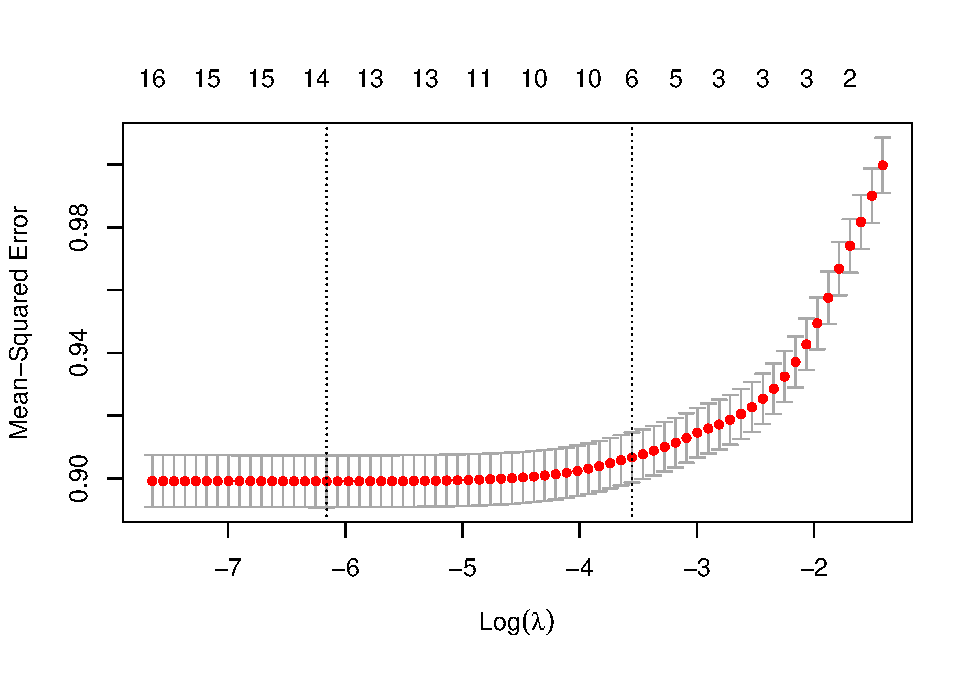
\includegraphics{../results/report_files/figure-latex/statin-lasso-plot-1.pdf}

\begin{Shaded}
\begin{Highlighting}[]
\FunctionTok{coef}\NormalTok{(statin.glmnet.cv, }\FunctionTok{c}\NormalTok{(statin.glmnet.cv}\SpecialCharTok{$}\NormalTok{lambda.min,}
\NormalTok{                   statin.glmnet.cv}\SpecialCharTok{$}\NormalTok{lambda}\FloatTok{.1}\NormalTok{se))}
\end{Highlighting}
\end{Shaded}

\begin{verbatim}
## 17 x 2 sparse Matrix of class "dgCMatrix"
##                                    s1            s2
## (Intercept)             -2.275099e-16 -1.080653e-16
## SID                      6.956339e-04  .           
## SexMale                  2.260680e-02  .           
## Age                     -4.736318e-02  .           
## packyrs                  3.460619e-02  7.207680e-03
## alcoholintakegpd         2.768395e-03  .           
## PriorMed                 .             .           
## HypertensionTRUE         3.887463e-02  1.273594e-02
## ObesityTRUE             -9.817050e-03  .           
## `Diabetes Mellitus`TRUE  1.989265e-02  .           
## CADTRUE                  1.123753e-02  .           
## HypercholTRUE           -5.070867e-03  .           
## `Heart Failure`TRUE      .             .           
## bmi                     -8.337809e-02 -3.636707e-02
## sbp                      1.542788e-01  1.182037e-01
## dbp                      1.232901e-01  1.244400e-01
## pulse_rate               1.640762e-01  1.306085e-01
\end{verbatim}

\hypertarget{metformin}{%
\subsection{Metformin}\label{metformin}}

\begin{Shaded}
\begin{Highlighting}[]
\NormalTok{metformin.df }\OtherTok{\textless{}{-}}\NormalTok{ dfs }\SpecialCharTok{\%\textgreater{}\%} 
  \FunctionTok{filter}\NormalTok{(Drug}\SpecialCharTok{==}\StringTok{"Metformin"}\NormalTok{) }\SpecialCharTok{\%\textgreater{}\%} 
  \FunctionTok{select}\NormalTok{(}\SpecialCharTok{{-}}\NormalTok{Drug)}
\end{Highlighting}
\end{Shaded}

\begin{Shaded}
\begin{Highlighting}[]
\NormalTok{metformin.fits.df }\OtherTok{\textless{}{-}}\NormalTok{ fits.df }\SpecialCharTok{\%\textgreater{}\%} 
  \FunctionTok{filter}\NormalTok{(Drug}\SpecialCharTok{==}\StringTok{"Metformin"}\NormalTok{)}
\end{Highlighting}
\end{Shaded}

\begin{Shaded}
\begin{Highlighting}[]
\FunctionTok{get\_pretty\_fit\_table}\NormalTok{(metformin.fits.df, }\StringTok{"Metformin"}\NormalTok{)}
\end{Highlighting}
\end{Shaded}

\begin{table}

\caption{\label{tab:metformin-fit-table}Metformin: Coefficients from linear models}
\centering
\begin{tabular}[t]{l|r|r|r|r|r|r|l}
\hline
term & estimate & std.error & statistic & p.value & conf.low & conf.high & Adjustment\\
\hline
(Intercept) & -20.492 & 0.517 & -39.642 & 0.000 & -21.505 & -19.479 & With SBP/DBP/HR\\
\hline
(Intercept) & -0.839 & 0.359 & -2.336 & 0.019 & -1.543 & -0.135 & Without SBP/DBP/HR\\
\hline
`Diabetes Mellitus`TRUE & 0.286 & 0.234 & 1.218 & 0.223 & -0.174 & 0.745 & With SBP/DBP/HR\\
\hline
`Diabetes Mellitus`TRUE & 0.150 & 0.245 & 0.612 & 0.541 & -0.330 & 0.630 & Without SBP/DBP/HR\\
\hline
`Heart Failure`TRUE & 0.114 & 0.370 & 0.308 & 0.758 & -0.612 & 0.840 & With SBP/DBP/HR\\
\hline
`Heart Failure`TRUE & -0.117 & 0.387 & -0.302 & 0.763 & -0.876 & 0.642 & Without SBP/DBP/HR\\
\hline
alcoholintakegpd & 0.001 & 0.003 & 0.376 & 0.707 & -0.004 & 0.006 & With SBP/DBP/HR\\
\hline
alcoholintakegpd & 0.006 & 0.003 & 2.389 & 0.017 & 0.001 & 0.012 & Without SBP/DBP/HR\\
\hline
bmi & -0.147 & 0.014 & -10.550 & 0.000 & -0.174 & -0.120 & With SBP/DBP/HR\\
\hline
bmi & -0.001 & 0.014 & -0.104 & 0.918 & -0.029 & 0.026 & Without SBP/DBP/HR\\
\hline
CADTRUE & 0.461 & 0.176 & 2.615 & 0.009 & 0.116 & 0.807 & With SBP/DBP/HR\\
\hline
CADTRUE & -0.478 & 0.183 & -2.611 & 0.009 & -0.838 & -0.119 & Without SBP/DBP/HR\\
\hline
dbp & 0.088 & 0.006 & 14.052 & 0.000 & 0.075 & 0.100 & With SBP/DBP/HR\\
\hline
HypercholTRUE & -0.147 & 0.112 & -1.317 & 0.188 & -0.367 & 0.072 & With SBP/DBP/HR\\
\hline
HypercholTRUE & -0.236 & 0.117 & -2.019 & 0.044 & -0.465 & -0.007 & Without SBP/DBP/HR\\
\hline
HypertensionTRUE & 0.652 & 0.102 & 6.405 & 0.000 & 0.453 & 0.852 & With SBP/DBP/HR\\
\hline
HypertensionTRUE & 1.815 & 0.103 & 17.561 & 0.000 & 1.612 & 2.018 & Without SBP/DBP/HR\\
\hline
ObesityTRUE & -0.270 & 0.148 & -1.818 & 0.069 & -0.560 & 0.021 & With SBP/DBP/HR\\
\hline
ObesityTRUE & -0.753 & 0.155 & -4.863 & 0.000 & -1.056 & -0.449 & Without SBP/DBP/HR\\
\hline
packyrs & 0.023 & 0.004 & 6.018 & 0.000 & 0.015 & 0.030 & With SBP/DBP/HR\\
\hline
packyrs & 0.021 & 0.004 & 5.418 & 0.000 & 0.014 & 0.029 & Without SBP/DBP/HR\\
\hline
poly(Age, 2)1 & -68.470 & 8.356 & -8.194 & 0.000 & -84.849 & -52.091 & With SBP/DBP/HR\\
\hline
poly(Age, 2)1 & -24.417 & 7.936 & -3.077 & 0.002 & -39.971 & -8.862 & Without SBP/DBP/HR\\
\hline
poly(Age, 2)2 & -106.349 & 7.246 & -14.676 & 0.000 & -120.552 & -92.146 & With SBP/DBP/HR\\
\hline
poly(Age, 2)2 & -113.168 & 7.562 & -14.965 & 0.000 & -127.991 & -98.346 & Without SBP/DBP/HR\\
\hline
PriorMed & 0.799 & 0.325 & 2.456 & 0.014 & 0.161 & 1.437 & With SBP/DBP/HR\\
\hline
PriorMed & 0.952 & 0.340 & 2.799 & 0.005 & 0.285 & 1.618 & Without SBP/DBP/HR\\
\hline
pulse\_rate & 0.110 & 0.004 & 27.703 & 0.000 & 0.102 & 0.118 & With SBP/DBP/HR\\
\hline
sbp & 0.067 & 0.003 & 19.608 & 0.000 & 0.061 & 0.074 & With SBP/DBP/HR\\
\hline
SexMale & 0.442 & 0.095 & 4.668 & 0.000 & 0.256 & 0.628 & With SBP/DBP/HR\\
\hline
SexMale & 0.515 & 0.096 & 5.370 & 0.000 & 0.327 & 0.704 & Without SBP/DBP/HR\\
\hline
\end{tabular}
\end{table}

\begin{Shaded}
\begin{Highlighting}[]
\FunctionTok{get\_pretty\_fit\_forest\_plot}\NormalTok{(metformin.fits.df) }\OtherTok{{-}\textgreater{}}\NormalTok{p}
\NormalTok{p}
\end{Highlighting}
\end{Shaded}

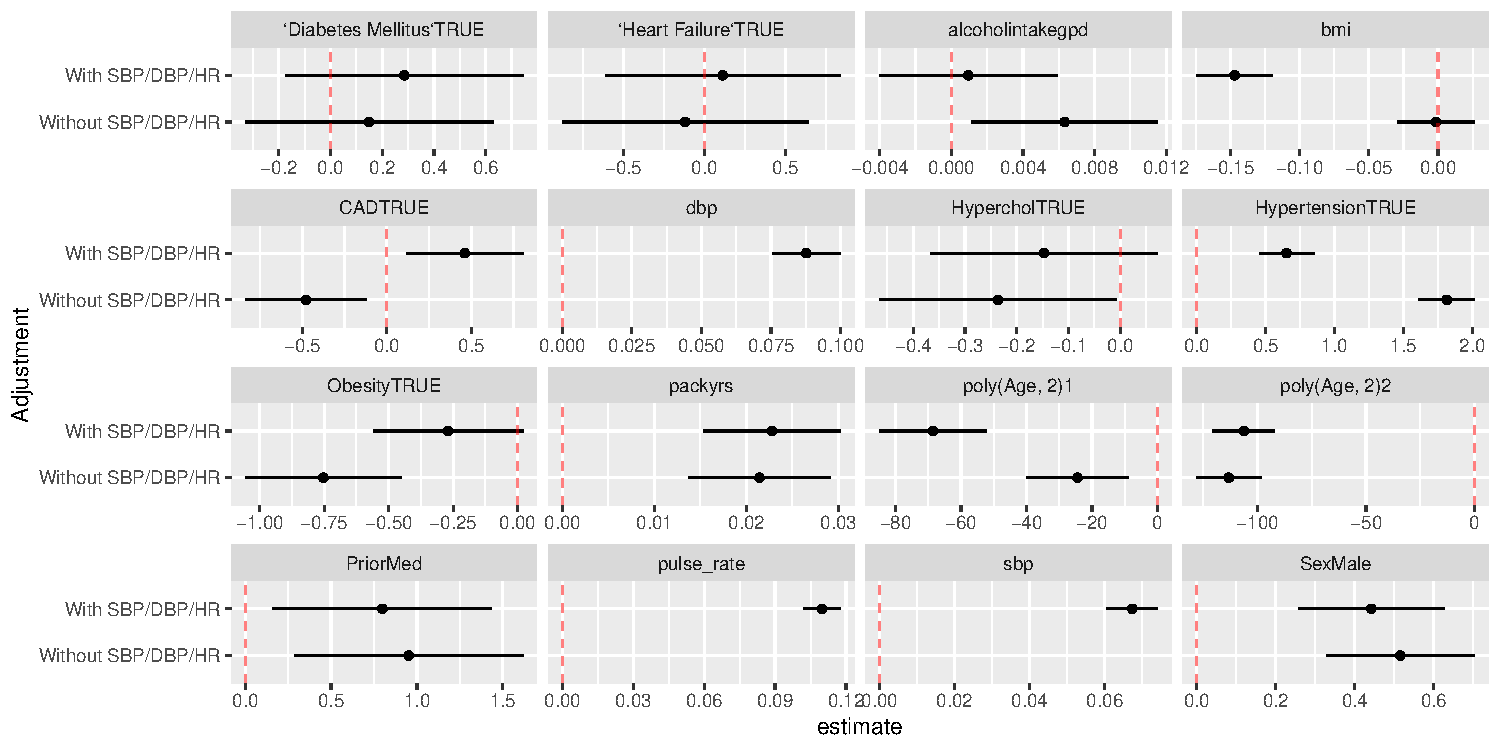
\includegraphics{../results/report_files/figure-latex/metformin-fit-forest-1.pdf}

\begin{Shaded}
\begin{Highlighting}[]
\NormalTok{metformin.fits.df }\SpecialCharTok{\%\textgreater{}\%} 
\NormalTok{  get\_fit\_glance}
\end{Highlighting}
\end{Shaded}

\begin{verbatim}
## # A tibble: 2 x 5
##   AdditionalMarkers     N fracPriorMed adj.r.squared r.squared
##   <lgl>             <dbl>        <dbl>         <dbl>     <dbl>
## 1 FALSE             27546        0.035         0.024     0.025
## 2 TRUE              27546        0.035         0.109     0.109
\end{verbatim}

\begin{Shaded}
\begin{Highlighting}[]
\FunctionTok{generate\_table.self.reported}\NormalTok{(metformin.df, }\StringTok{"Metformin"}\NormalTok{)}
\end{Highlighting}
\end{Shaded}

\begin{verbatim}
## Table printed with `knitr::kable()`, not {gt}. Learn why at
## https://www.danieldsjoberg.com/gtsummary/articles/rmarkdown.html
## To suppress this message, include `message = FALSE` in code chunk header.
\end{verbatim}

\begin{tabular}{l|c|c|c}
\hline
**Characteristic** & **Metformin**, N = 967 & **No Metformin**, N = 26,579 & **p-value**\\
\hline
Cardiac Age gap & 1.4 (-3.7, 6.8) & 0.1 (-5.4, 5.3) & <0.001\\
\hline
Sex &  &  & <0.001\\
\hline
Female & 299 (31\%) & 13,538 (51\%) & \\
\hline
Male & 668 (69\%) & 13,041 (49\%) & \\
\hline
Age & 66 (60, 71) & 64 (58, 70) & <0.001\\
\hline
Packs year of smoking & 0 (0, 13) & 0 (0, 3) & <0.001\\
\hline
Alcohol is g/day consumed & 1 (0, 11) & 4 (0, 15) & <0.001\\
\hline
Hypertension & 630 (65\%) & 8,568 (32\%) & <0.001\\
\hline
Obesity & 541 (56\%) & 5,134 (19\%) & <0.001\\
\hline
Diabetes Mellitus & 967 (100\%) & 1,016 (3.8\%) & <0.001\\
\hline
Coronary Artery Disease & 174 (18\%) & 1,934 (7.3\%) & <0.001\\
\hline
Hypercholesterolemia & 516 (53\%) & 5,775 (22\%) & <0.001\\
\hline
Heart Failure & 38 (3.9\%) & 374 (1.4\%) & <0.001\\
\hline
dbp & 78 (71, 84) & 78 (72, 86) & 0.005\\
\hline
sbp & 140 (130, 153) & 138 (126, 150) & <0.001\\
\hline
pulse\_rate & 73 (65, 83) & 68 (60, 76) & <0.001\\
\hline
bmi & 29.7 (26.7, 33.5) & 26.2 (23.7, 29.1) & <0.001\\
\hline
\end{tabular}

\begin{Shaded}
\begin{Highlighting}[]
\NormalTok{metformin.df }\SpecialCharTok{\%\textgreater{}\%} 
  \FunctionTok{get\_stratified\_age\_gap\_histogram}\NormalTok{(}\StringTok{"Metformin"}\NormalTok{)}
\end{Highlighting}
\end{Shaded}

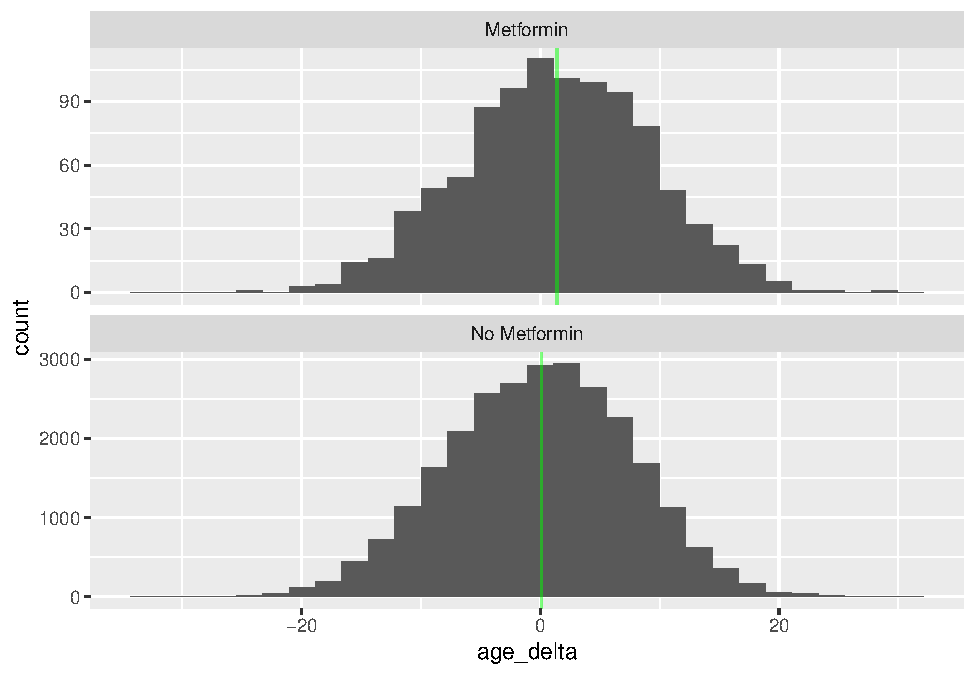
\includegraphics{../results/report_files/figure-latex/metformin-age-gap-histograms-1.pdf}

\begin{Shaded}
\begin{Highlighting}[]
\NormalTok{metformin.df }\SpecialCharTok{\%\textgreater{}\%} 
    \FunctionTok{get\_stratified\_age\_gap\_quantiles}\NormalTok{(}\StringTok{"Metformin"}\NormalTok{)}
\end{Highlighting}
\end{Shaded}

\begin{verbatim}
## # A tibble: 2 x 9
##   PriorMed      `1%` `2.5%` `25%` `50%` `75%` `97.5%` `99%`     N
##   <chr>        <dbl>  <dbl> <dbl> <dbl> <dbl>   <dbl> <dbl> <int>
## 1 Metformin    -16.1  -14.0 -3.73  1.41  6.78    16.4  18.2   967
## 2 No Metformin -17.8  -15.1 -5.35  0.12  5.28    14.3  16.8 26579
\end{verbatim}

\hypertarget{lasso-1}{%
\subsubsection{Lasso}\label{lasso-1}}

\begin{Shaded}
\begin{Highlighting}[]
\NormalTok{metformin.glmnet.cv }\OtherTok{\textless{}{-}}\NormalTok{ fits.glm[[}\StringTok{"Metformin"}\NormalTok{]]}
\end{Highlighting}
\end{Shaded}

\begin{Shaded}
\begin{Highlighting}[]
\FunctionTok{plot}\NormalTok{(metformin.glmnet.cv) }
\end{Highlighting}
\end{Shaded}

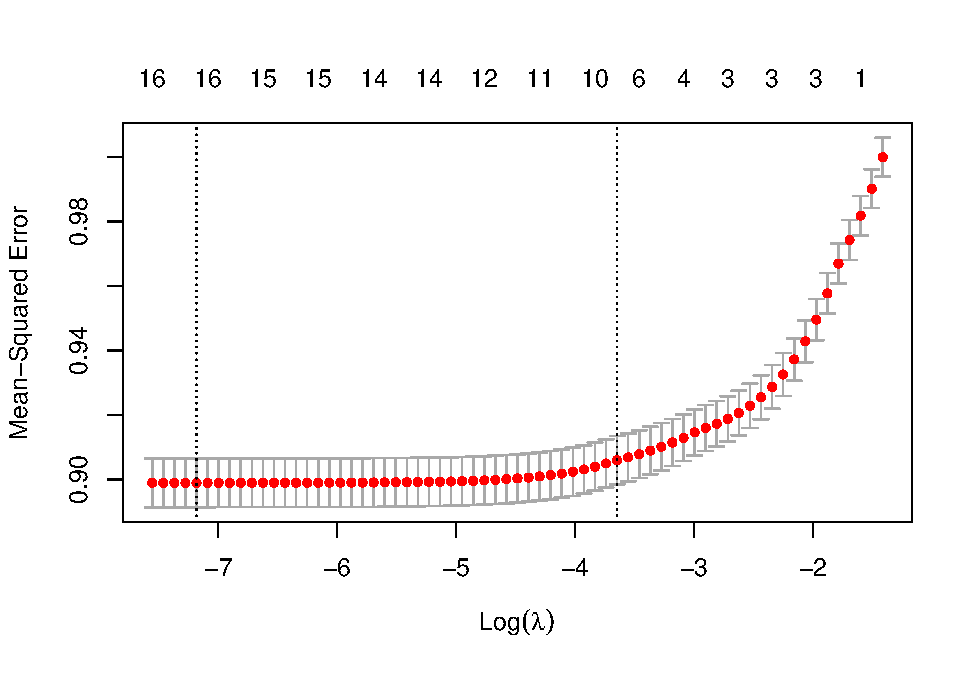
\includegraphics{../results/report_files/figure-latex/statin-metformin-plot-1.pdf}

\begin{Shaded}
\begin{Highlighting}[]
\FunctionTok{coef}\NormalTok{(metformin.glmnet.cv, }\FunctionTok{c}\NormalTok{(metformin.glmnet.cv}\SpecialCharTok{$}\NormalTok{lambda.min,}
\NormalTok{                   metformin.glmnet.cv}\SpecialCharTok{$}\NormalTok{lambda}\FloatTok{.1}\NormalTok{se))}
\end{Highlighting}
\end{Shaded}

\begin{verbatim}
## 17 x 2 sparse Matrix of class "dgCMatrix"
##                                    s1            s2
## (Intercept)             -1.919073e-16 -1.144220e-16
## SID                      1.997608e-03  .           
## SexMale                  2.326247e-02  .           
## Age                     -4.960966e-02 -3.901188e-04
## packyrs                  3.571725e-02  1.000863e-02
## alcoholintakegpd         3.916300e-03  .           
## PriorMed                 1.948702e-02  .           
## HypertensionTRUE         4.019460e-02  1.517539e-02
## ObesityTRUE             -1.121007e-02  .           
## `Diabetes Mellitus`TRUE  8.450938e-03  .           
## CADTRUE                  1.318581e-02  .           
## HypercholTRUE           -7.544698e-03  .           
## `Heart Failure`TRUE      1.049425e-04  .           
## bmi                     -8.587474e-02 -4.076007e-02
## sbp                      1.559864e-01  1.195392e-01
## dbp                      1.237520e-01  1.262449e-01
## pulse_rate               1.652048e-01  1.331395e-01
\end{verbatim}

\hypertarget{digoxin}{%
\subsection{Digoxin}\label{digoxin}}

\begin{Shaded}
\begin{Highlighting}[]
\NormalTok{digoxin.df }\OtherTok{\textless{}{-}}\NormalTok{ dfs }\SpecialCharTok{\%\textgreater{}\%} 
  \FunctionTok{filter}\NormalTok{(Drug}\SpecialCharTok{==}\StringTok{"Digoxin"}\NormalTok{) }\SpecialCharTok{\%\textgreater{}\%} 
  \FunctionTok{select}\NormalTok{(}\SpecialCharTok{{-}}\NormalTok{Drug)}
\end{Highlighting}
\end{Shaded}

\begin{Shaded}
\begin{Highlighting}[]
\NormalTok{digoxin.fits.df }\OtherTok{\textless{}{-}}\NormalTok{ fits.df }\SpecialCharTok{\%\textgreater{}\%} 
  \FunctionTok{filter}\NormalTok{(Drug}\SpecialCharTok{==}\StringTok{"Digoxin"}\NormalTok{)}
\end{Highlighting}
\end{Shaded}

\begin{Shaded}
\begin{Highlighting}[]
\FunctionTok{get\_pretty\_fit\_table}\NormalTok{(digoxin.fits.df, }\StringTok{"Digoxin"}\NormalTok{)}
\end{Highlighting}
\end{Shaded}

\begin{table}

\caption{\label{tab:digoxin-fit-table}Digoxin: Coefficients from linear models}
\centering
\begin{tabular}[t]{l|r|r|r|r|r|r|l}
\hline
term & estimate & std.error & statistic & p.value & conf.low & conf.high & Adjustment\\
\hline
(Intercept) & -20.518 & 0.517 & -39.695 & 0.000 & -21.531 & -19.504 & With SBP/DBP/HR\\
\hline
(Intercept) & -0.858 & 0.359 & -2.390 & 0.017 & -1.562 & -0.154 & Without SBP/DBP/HR\\
\hline
`Diabetes Mellitus`TRUE & 0.662 & 0.176 & 3.755 & 0.000 & 0.317 & 1.008 & With SBP/DBP/HR\\
\hline
`Diabetes Mellitus`TRUE & 0.601 & 0.183 & 3.276 & 0.001 & 0.241 & 0.960 & Without SBP/DBP/HR\\
\hline
`Heart Failure`TRUE & 0.088 & 0.372 & 0.237 & 0.813 & -0.642 & 0.818 & With SBP/DBP/HR\\
\hline
`Heart Failure`TRUE & -0.152 & 0.390 & -0.391 & 0.696 & -0.916 & 0.611 & Without SBP/DBP/HR\\
\hline
alcoholintakegpd & 0.001 & 0.003 & 0.323 & 0.747 & -0.004 & 0.006 & With SBP/DBP/HR\\
\hline
alcoholintakegpd & 0.006 & 0.003 & 2.328 & 0.020 & 0.001 & 0.011 & Without SBP/DBP/HR\\
\hline
bmi & -0.147 & 0.014 & -10.522 & 0.000 & -0.174 & -0.119 & With SBP/DBP/HR\\
\hline
bmi & -0.001 & 0.014 & -0.072 & 0.942 & -0.029 & 0.027 & Without SBP/DBP/HR\\
\hline
CADTRUE & 0.458 & 0.176 & 2.594 & 0.009 & 0.112 & 0.803 & With SBP/DBP/HR\\
\hline
CADTRUE & -0.483 & 0.183 & -2.637 & 0.008 & -0.842 & -0.124 & Without SBP/DBP/HR\\
\hline
dbp & 0.087 & 0.006 & 13.981 & 0.000 & 0.075 & 0.099 & With SBP/DBP/HR\\
\hline
HypercholTRUE & -0.140 & 0.112 & -1.250 & 0.211 & -0.359 & 0.079 & With SBP/DBP/HR\\
\hline
HypercholTRUE & -0.226 & 0.117 & -1.936 & 0.053 & -0.456 & 0.003 & Without SBP/DBP/HR\\
\hline
HypertensionTRUE & 0.655 & 0.102 & 6.429 & 0.000 & 0.455 & 0.854 & With SBP/DBP/HR\\
\hline
HypertensionTRUE & 1.818 & 0.103 & 17.584 & 0.000 & 1.615 & 2.020 & Without SBP/DBP/HR\\
\hline
ObesityTRUE & -0.257 & 0.148 & -1.737 & 0.082 & -0.548 & 0.033 & With SBP/DBP/HR\\
\hline
ObesityTRUE & -0.738 & 0.155 & -4.771 & 0.000 & -1.042 & -0.435 & Without SBP/DBP/HR\\
\hline
packyrs & 0.023 & 0.004 & 6.047 & 0.000 & 0.015 & 0.030 & With SBP/DBP/HR\\
\hline
packyrs & 0.022 & 0.004 & 5.458 & 0.000 & 0.014 & 0.029 & Without SBP/DBP/HR\\
\hline
poly(Age, 2)1 & -68.835 & 8.358 & -8.235 & 0.000 & -85.218 & -52.452 & With SBP/DBP/HR\\
\hline
poly(Age, 2)1 & -24.680 & 7.938 & -3.109 & 0.002 & -40.238 & -9.122 & Without SBP/DBP/HR\\
\hline
poly(Age, 2)2 & -106.512 & 7.248 & -14.696 & 0.000 & -120.718 & -92.306 & With SBP/DBP/HR\\
\hline
poly(Age, 2)2 & -113.329 & 7.564 & -14.983 & 0.000 & -128.155 & -98.503 & Without SBP/DBP/HR\\
\hline
PriorMed & 0.550 & 1.212 & 0.454 & 0.650 & -1.825 & 2.924 & With SBP/DBP/HR\\
\hline
PriorMed & 0.815 & 1.268 & 0.643 & 0.520 & -1.669 & 3.300 & Without SBP/DBP/HR\\
\hline
pulse\_rate & 0.110 & 0.004 & 27.838 & 0.000 & 0.102 & 0.118 & With SBP/DBP/HR\\
\hline
sbp & 0.067 & 0.003 & 19.635 & 0.000 & 0.061 & 0.074 & With SBP/DBP/HR\\
\hline
SexMale & 0.450 & 0.095 & 4.754 & 0.000 & 0.264 & 0.635 & With SBP/DBP/HR\\
\hline
SexMale & 0.521 & 0.096 & 5.433 & 0.000 & 0.333 & 0.710 & Without SBP/DBP/HR\\
\hline
\end{tabular}
\end{table}

\begin{Shaded}
\begin{Highlighting}[]
\FunctionTok{get\_pretty\_fit\_forest\_plot}\NormalTok{(digoxin.fits.df) }\OtherTok{{-}\textgreater{}}\NormalTok{p}
\NormalTok{p}
\end{Highlighting}
\end{Shaded}

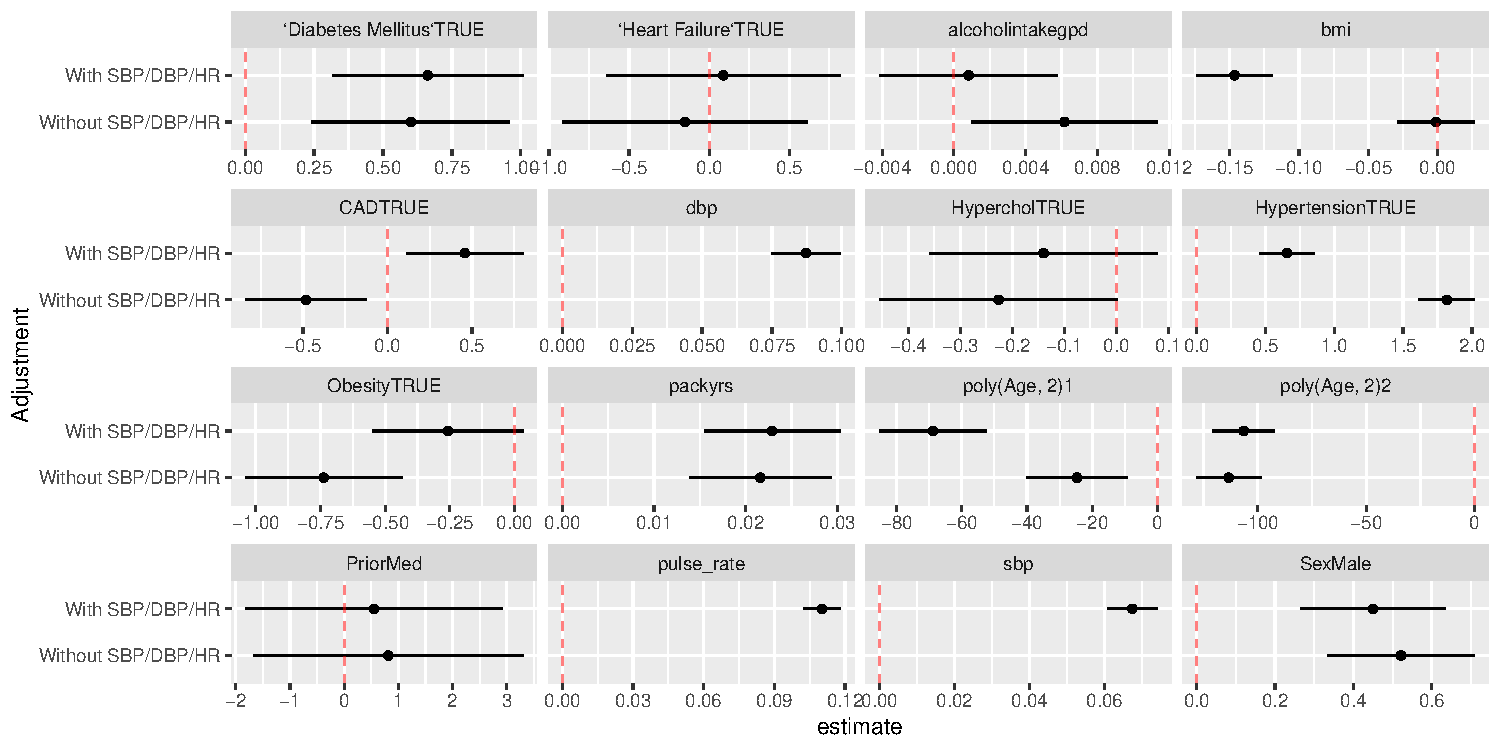
\includegraphics{../results/report_files/figure-latex/digoxin-fit-forest-1.pdf}

\begin{Shaded}
\begin{Highlighting}[]
\NormalTok{digoxin.fits.df }\SpecialCharTok{\%\textgreater{}\%} 
\NormalTok{  get\_fit\_glance}
\end{Highlighting}
\end{Shaded}

\begin{verbatim}
## # A tibble: 2 x 5
##   AdditionalMarkers     N fracPriorMed adj.r.squared r.squared
##   <lgl>             <dbl>        <dbl>         <dbl>     <dbl>
## 1 FALSE             27546        0.001         0.024     0.024
## 2 TRUE              27546        0.001         0.108     0.109
\end{verbatim}

\begin{Shaded}
\begin{Highlighting}[]
\FunctionTok{generate\_table.self.reported}\NormalTok{(digoxin.df, }\StringTok{"Digoxin"}\NormalTok{)}
\end{Highlighting}
\end{Shaded}

\begin{verbatim}
## Table printed with `knitr::kable()`, not {gt}. Learn why at
## https://www.danieldsjoberg.com/gtsummary/articles/rmarkdown.html
## To suppress this message, include `message = FALSE` in code chunk header.
\end{verbatim}

\begin{tabular}{l|c|c|c}
\hline
**Characteristic** & **Digoxin**, N = 36 & **No Digoxin**, N = 27,510 & **p-value**\\
\hline
Cardiac Age gap & 1.5 (-4.9, 6.7) & 0.2 (-5.3, 5.3) & 0.5\\
\hline
Sex &  &  & <0.001\\
\hline
Female & 8 (22\%) & 13,829 (50\%) & \\
\hline
Male & 28 (78\%) & 13,681 (50\%) & \\
\hline
Age & 71 (66, 75) & 65 (58, 70) & <0.001\\
\hline
Packs year of smoking & 0 (0, 8) & 0 (0, 3) & 0.6\\
\hline
Alcohol is g/day consumed & 2 (0, 17) & 4 (0, 15) & 0.7\\
\hline
Hypertension & 23 (64\%) & 9,175 (33\%) & <0.001\\
\hline
Obesity & 12 (33\%) & 5,663 (21\%) & 0.059\\
\hline
Diabetes Mellitus & 13 (36\%) & 1,970 (7.2\%) & <0.001\\
\hline
Coronary Artery Disease & 8 (22\%) & 2,100 (7.6\%) & 0.005\\
\hline
Hypercholesterolemia & 12 (33\%) & 6,279 (23\%) & 0.13\\
\hline
Heart Failure & 14 (39\%) & 398 (1.4\%) & <0.001\\
\hline
dbp & 77 (71, 88) & 78 (72, 86) & >0.9\\
\hline
sbp & 136 (124, 156) & 138 (126, 150) & 0.8\\
\hline
pulse\_rate & 74 (66, 82) & 68 (61, 76) & 0.006\\
\hline
bmi & 27.3 (23.9, 31.7) & 26.3 (23.8, 29.3) & 0.3\\
\hline
\end{tabular}

\begin{Shaded}
\begin{Highlighting}[]
\NormalTok{digoxin.df }\SpecialCharTok{\%\textgreater{}\%} 
  \FunctionTok{get\_stratified\_age\_gap\_histogram}\NormalTok{(}\StringTok{"Digoxin"}\NormalTok{)}
\end{Highlighting}
\end{Shaded}

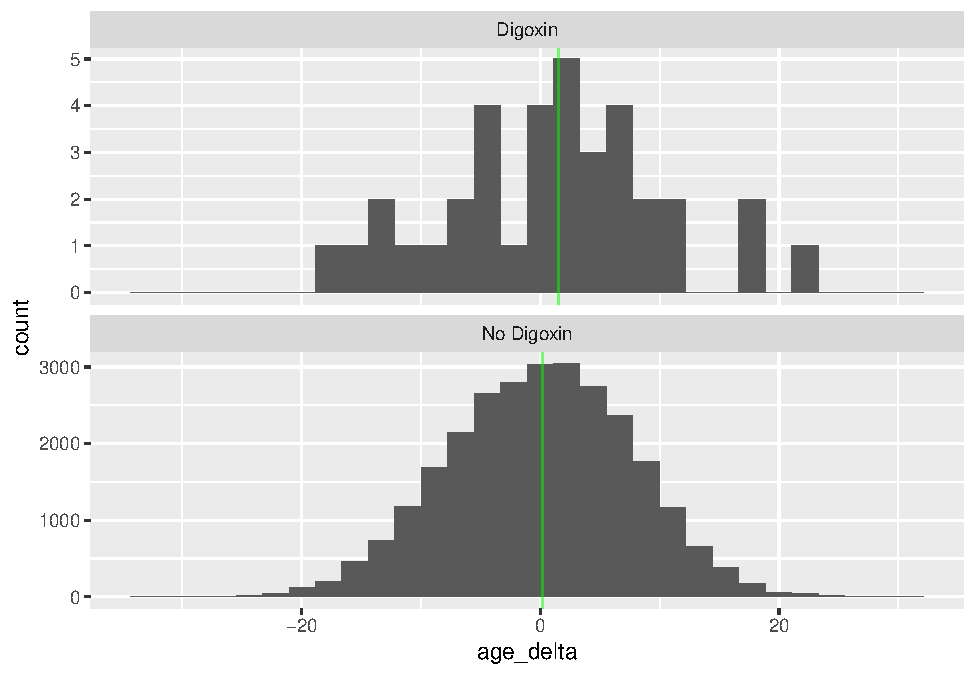
\includegraphics{../results/report_files/figure-latex/digoxin-age-gap-histograms-1.pdf}

\begin{Shaded}
\begin{Highlighting}[]
\NormalTok{digoxin.df }\SpecialCharTok{\%\textgreater{}\%} 
  \FunctionTok{get\_stratified\_age\_gap\_quantiles}\NormalTok{(}\StringTok{"Digoxin"}\NormalTok{)}
\end{Highlighting}
\end{Shaded}

\begin{verbatim}
## # A tibble: 2 x 9
##   PriorMed    `1%` `2.5%` `25%` `50%` `75%` `97.5%` `99%`     N
##   <chr>      <dbl>  <dbl> <dbl> <dbl> <dbl>   <dbl> <dbl> <int>
## 1 Digoxin    -16.6  -16.1 -4.86  1.53  6.73    18.9  20.8    36
## 2 No Digoxin -17.7  -15.0 -5.3   0.16  5.33    14.4  16.9 27510
\end{verbatim}

\hypertarget{lasso-2}{%
\subsubsection{Lasso}\label{lasso-2}}

\begin{Shaded}
\begin{Highlighting}[]
\NormalTok{digoxin.glmnet.cv }\OtherTok{\textless{}{-}}\NormalTok{ fits.glm[[}\StringTok{"Digoxin"}\NormalTok{]]}
\end{Highlighting}
\end{Shaded}

\begin{Shaded}
\begin{Highlighting}[]
\FunctionTok{plot}\NormalTok{(digoxin.glmnet.cv) }
\end{Highlighting}
\end{Shaded}

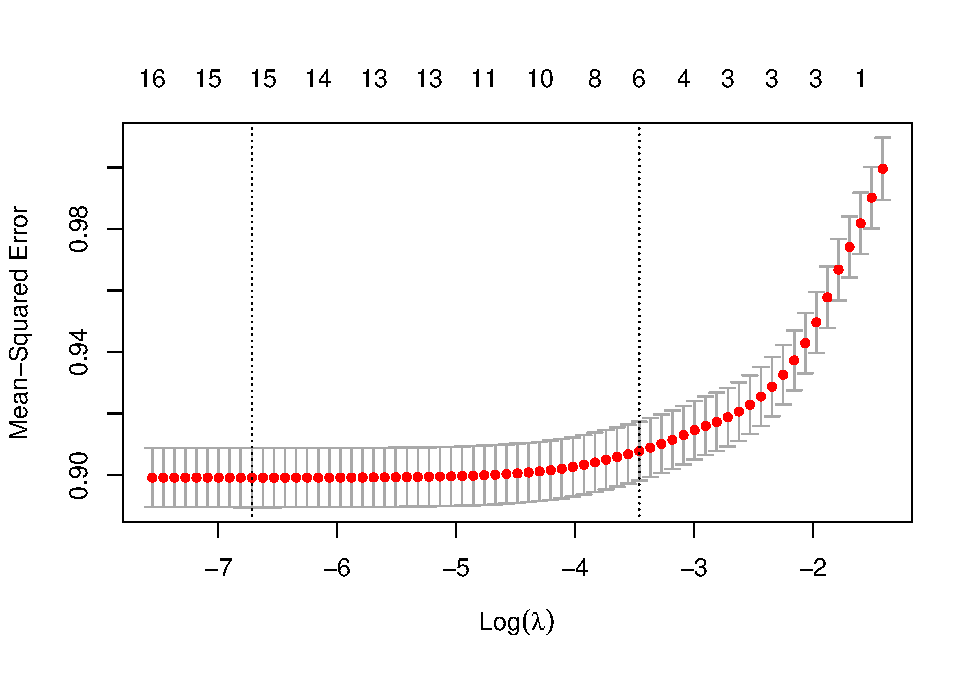
\includegraphics{../results/report_files/figure-latex/digoxin-lasso-plot-1.pdf}

\begin{Shaded}
\begin{Highlighting}[]
\FunctionTok{coef}\NormalTok{(digoxin.glmnet.cv, }\FunctionTok{c}\NormalTok{(digoxin.glmnet.cv}\SpecialCharTok{$}\NormalTok{lambda.min,}
\NormalTok{                   digoxin.glmnet.cv}\SpecialCharTok{$}\NormalTok{lambda}\FloatTok{.1}\NormalTok{se))}
\end{Highlighting}
\end{Shaded}

\begin{verbatim}
## 17 x 2 sparse Matrix of class "dgCMatrix"
##                                    s1            s2
## (Intercept)             -2.330190e-16 -1.012851e-16
## SID                      1.638825e-03  .           
## SexMale                  2.340433e-02  .           
## Age                     -4.899890e-02  .           
## packyrs                  3.546793e-02  4.173688e-03
## alcoholintakegpd         3.335993e-03  .           
## PriorMed                 2.639928e-04  .           
## HypertensionTRUE         3.987529e-02  1.019900e-02
## ObesityTRUE             -1.031775e-02  .           
## `Diabetes Mellitus`TRUE  2.092399e-02  .           
## CADTRUE                  1.241705e-02  .           
## HypercholTRUE           -6.457367e-03  .           
## `Heart Failure`TRUE      .             .           
## bmi                     -8.489514e-02 -3.159110e-02
## sbp                      1.555273e-01  1.167419e-01
## dbp                      1.232406e-01  1.224064e-01
## pulse_rate               1.652914e-01  1.278304e-01
\end{verbatim}

\hypertarget{beta-blocker}{%
\subsection{Beta Blocker}\label{beta-blocker}}

\begin{Shaded}
\begin{Highlighting}[]
\NormalTok{BB.df }\OtherTok{\textless{}{-}}\NormalTok{ dfs }\SpecialCharTok{\%\textgreater{}\%} 
  \FunctionTok{filter}\NormalTok{(Drug}\SpecialCharTok{==}\StringTok{"BB"}\NormalTok{) }\SpecialCharTok{\%\textgreater{}\%} 
  \FunctionTok{select}\NormalTok{(}\SpecialCharTok{{-}}\NormalTok{Drug)}
\end{Highlighting}
\end{Shaded}

\begin{Shaded}
\begin{Highlighting}[]
\NormalTok{BB.fits.df }\OtherTok{\textless{}{-}}\NormalTok{ fits.df }\SpecialCharTok{\%\textgreater{}\%} 
  \FunctionTok{filter}\NormalTok{(Drug}\SpecialCharTok{==}\StringTok{"BB"}\NormalTok{)}
\end{Highlighting}
\end{Shaded}

\begin{Shaded}
\begin{Highlighting}[]
\FunctionTok{get\_pretty\_fit\_table}\NormalTok{(BB.fits.df, }\StringTok{"Beta Blocker"}\NormalTok{)}
\end{Highlighting}
\end{Shaded}

\begin{table}

\caption{\label{tab:BB-fit-table}Beta Blocker: Coefficients from linear models}
\centering
\begin{tabular}[t]{l|r|r|r|r|r|r|l}
\hline
term & estimate & std.error & statistic & p.value & conf.low & conf.high & Adjustment\\
\hline
(Intercept) & -20.673 & 0.519 & -39.825 & 0.000 & -21.690 & -19.655 & With SBP/DBP/HR\\
\hline
(Intercept) & -0.893 & 0.359 & -2.486 & 0.013 & -1.596 & -0.189 & Without SBP/DBP/HR\\
\hline
`Diabetes Mellitus`TRUE & 0.649 & 0.176 & 3.681 & 0.000 & 0.304 & 0.995 & With SBP/DBP/HR\\
\hline
`Diabetes Mellitus`TRUE & 0.620 & 0.183 & 3.385 & 0.001 & 0.261 & 0.980 & Without SBP/DBP/HR\\
\hline
`Heart Failure`TRUE & 0.015 & 0.371 & 0.041 & 0.967 & -0.713 & 0.743 & With SBP/DBP/HR\\
\hline
`Heart Failure`TRUE & -0.001 & 0.388 & -0.002 & 0.999 & -0.762 & 0.761 & Without SBP/DBP/HR\\
\hline
alcoholintakegpd & 0.001 & 0.003 & 0.293 & 0.770 & -0.004 & 0.006 & With SBP/DBP/HR\\
\hline
alcoholintakegpd & 0.006 & 0.003 & 2.355 & 0.019 & 0.001 & 0.011 & Without SBP/DBP/HR\\
\hline
bmi & -0.149 & 0.014 & -10.691 & 0.000 & -0.176 & -0.122 & With SBP/DBP/HR\\
\hline
bmi & 0.001 & 0.014 & 0.046 & 0.963 & -0.027 & 0.029 & Without SBP/DBP/HR\\
\hline
CADTRUE & 0.281 & 0.185 & 1.524 & 0.128 & -0.081 & 0.643 & With SBP/DBP/HR\\
\hline
CADTRUE & -0.235 & 0.193 & -1.219 & 0.223 & -0.613 & 0.143 & Without SBP/DBP/HR\\
\hline
dbp & 0.087 & 0.006 & 14.008 & 0.000 & 0.075 & 0.100 & With SBP/DBP/HR\\
\hline
HypercholTRUE & -0.158 & 0.112 & -1.416 & 0.157 & -0.378 & 0.061 & With SBP/DBP/HR\\
\hline
HypercholTRUE & -0.203 & 0.117 & -1.733 & 0.083 & -0.432 & 0.027 & Without SBP/DBP/HR\\
\hline
HypertensionTRUE & 0.609 & 0.103 & 5.925 & 0.000 & 0.408 & 0.811 & With SBP/DBP/HR\\
\hline
HypertensionTRUE & 1.868 & 0.104 & 17.961 & 0.000 & 1.664 & 2.072 & Without SBP/DBP/HR\\
\hline
ObesityTRUE & -0.256 & 0.148 & -1.728 & 0.084 & -0.547 & 0.034 & With SBP/DBP/HR\\
\hline
ObesityTRUE & -0.734 & 0.155 & -4.744 & 0.000 & -1.037 & -0.431 & Without SBP/DBP/HR\\
\hline
packyrs & 0.023 & 0.004 & 6.047 & 0.000 & 0.015 & 0.030 & With SBP/DBP/HR\\
\hline
packyrs & 0.022 & 0.004 & 5.450 & 0.000 & 0.014 & 0.029 & Without SBP/DBP/HR\\
\hline
poly(Age, 2)1 & -70.335 & 8.370 & -8.404 & 0.000 & -86.740 & -53.930 & With SBP/DBP/HR\\
\hline
poly(Age, 2)1 & -23.089 & 7.942 & -2.907 & 0.004 & -38.656 & -7.522 & Without SBP/DBP/HR\\
\hline
poly(Age, 2)2 & -106.876 & 7.247 & -14.748 & 0.000 & -121.080 & -92.672 & With SBP/DBP/HR\\
\hline
poly(Age, 2)2 & -112.698 & 7.562 & -14.903 & 0.000 & -127.520 & -97.876 & Without SBP/DBP/HR\\
\hline
PriorMed & 0.606 & 0.190 & 3.182 & 0.001 & 0.233 & 0.979 & With SBP/DBP/HR\\
\hline
PriorMed & -0.818 & 0.196 & -4.165 & 0.000 & -1.203 & -0.433 & Without SBP/DBP/HR\\
\hline
pulse\_rate & 0.112 & 0.004 & 28.017 & 0.000 & 0.104 & 0.120 & With SBP/DBP/HR\\
\hline
sbp & 0.068 & 0.003 & 19.772 & 0.000 & 0.061 & 0.075 & With SBP/DBP/HR\\
\hline
SexMale & 0.455 & 0.095 & 4.806 & 0.000 & 0.269 & 0.640 & With SBP/DBP/HR\\
\hline
SexMale & 0.523 & 0.096 & 5.450 & 0.000 & 0.335 & 0.711 & Without SBP/DBP/HR\\
\hline
\end{tabular}
\end{table}

\begin{Shaded}
\begin{Highlighting}[]
\FunctionTok{get\_pretty\_fit\_forest\_plot}\NormalTok{(BB.fits.df) }\OtherTok{{-}\textgreater{}}\NormalTok{p}
\NormalTok{p}
\end{Highlighting}
\end{Shaded}

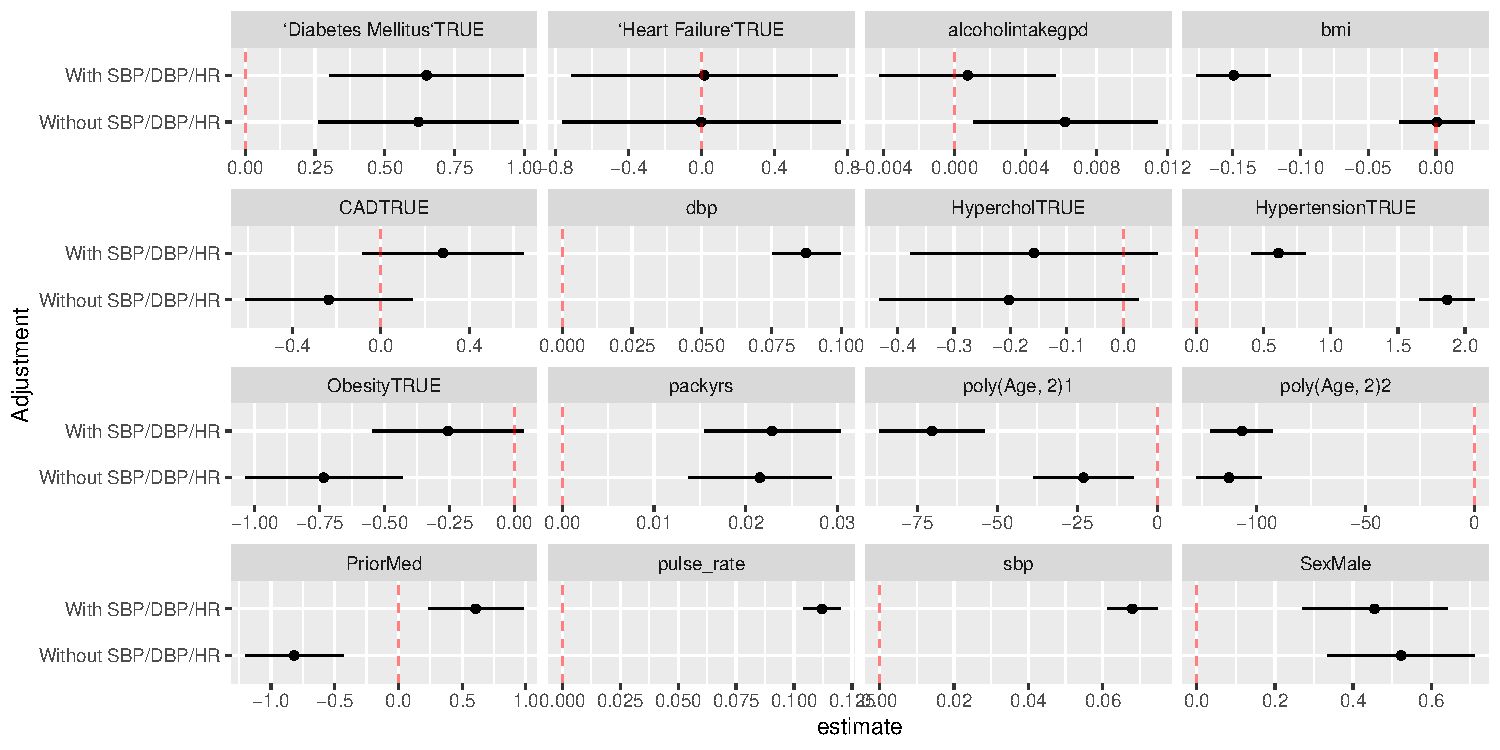
\includegraphics{../results/report_files/figure-latex/BB-fit-forest-1.pdf}

\begin{Shaded}
\begin{Highlighting}[]
\NormalTok{BB.fits.df }\SpecialCharTok{\%\textgreater{}\%} 
\NormalTok{  get\_fit\_glance}
\end{Highlighting}
\end{Shaded}

\begin{verbatim}
## # A tibble: 2 x 5
##   AdditionalMarkers     N fracPriorMed adj.r.squared r.squared
##   <lgl>             <dbl>        <dbl>         <dbl>     <dbl>
## 1 FALSE             27546         0.07         0.024     0.025
## 2 TRUE              27546         0.07         0.109     0.109
\end{verbatim}

\begin{Shaded}
\begin{Highlighting}[]
\FunctionTok{generate\_table.self.reported}\NormalTok{(BB.df, }\StringTok{"BB"}\NormalTok{)}
\end{Highlighting}
\end{Shaded}

\begin{verbatim}
## Table printed with `knitr::kable()`, not {gt}. Learn why at
## https://www.danieldsjoberg.com/gtsummary/articles/rmarkdown.html
## To suppress this message, include `message = FALSE` in code chunk header.
\end{verbatim}

\begin{tabular}{l|c|c|c}
\hline
**Characteristic** & **BB**, N = 1,918 & **No BB**, N = 25,628 & **p-value**\\
\hline
Cardiac Age gap & 0.0 (-5.3, 5.0) & 0.2 (-5.3, 5.4) & 0.2\\
\hline
Sex &  &  & <0.001\\
\hline
Female & 681 (36\%) & 13,156 (51\%) & \\
\hline
Male & 1,237 (64\%) & 12,472 (49\%) & \\
\hline
Age & 69 (63, 72) & 64 (58, 69) & <0.001\\
\hline
Packs year of smoking & 0 (0, 8) & 0 (0, 3) & <0.001\\
\hline
Alcohol is g/day consumed & 4 (0, 17) & 4 (0, 15) & 0.3\\
\hline
Hypertension & 1,262 (66\%) & 7,936 (31\%) & <0.001\\
\hline
Obesity & 587 (31\%) & 5,088 (20\%) & <0.001\\
\hline
Diabetes Mellitus & 315 (16\%) & 1,668 (6.5\%) & <0.001\\
\hline
Coronary Artery Disease & 843 (44\%) & 1,265 (4.9\%) & <0.001\\
\hline
Hypercholesterolemia & 935 (49\%) & 5,356 (21\%) & <0.001\\
\hline
Heart Failure & 171 (8.9\%) & 241 (0.9\%) & <0.001\\
\hline
dbp & 76 (70, 84) & 79 (72, 86) & <0.001\\
\hline
sbp & 138 (126, 152) & 138 (126, 150) & 0.12\\
\hline
pulse\_rate & 61 (55, 69) & 68 (62, 76) & <0.001\\
\hline
bmi & 27.7 (25.1, 30.9) & 26.2 (23.7, 29.1) & <0.001\\
\hline
\end{tabular}

\begin{Shaded}
\begin{Highlighting}[]
\NormalTok{BB.df }\SpecialCharTok{\%\textgreater{}\%} 
 \FunctionTok{get\_stratified\_age\_gap\_histogram}\NormalTok{(}\StringTok{"Beta Blockers"}\NormalTok{)}
\end{Highlighting}
\end{Shaded}

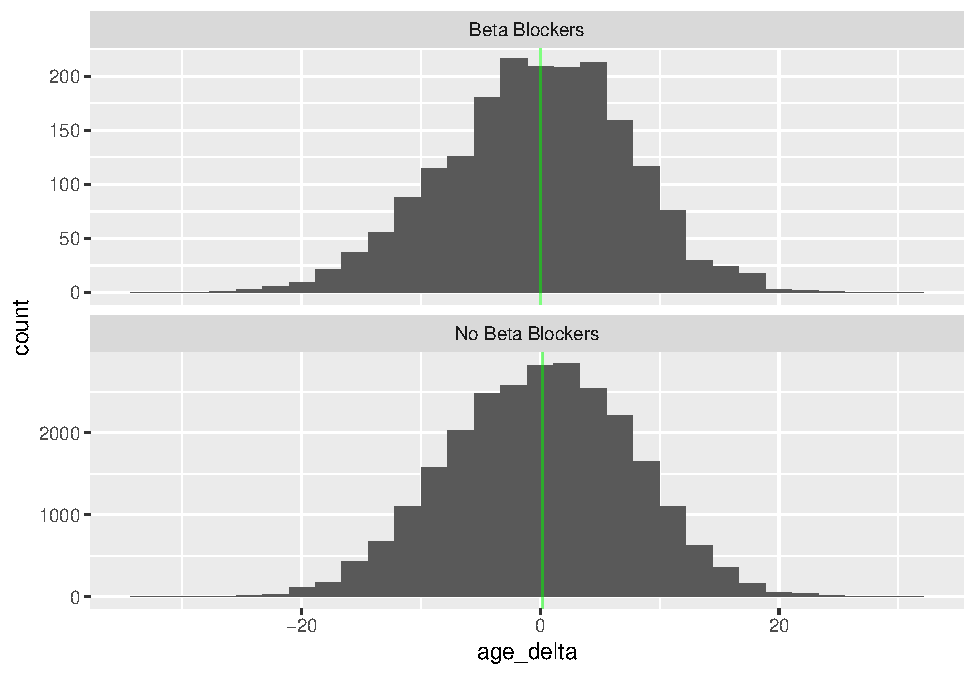
\includegraphics{../results/report_files/figure-latex/BB-age-gap-histograms-1.pdf}

\begin{Shaded}
\begin{Highlighting}[]
\NormalTok{BB.df }\SpecialCharTok{\%\textgreater{}\%} 
 \FunctionTok{get\_stratified\_age\_gap\_quantiles}\NormalTok{(}\StringTok{"Beta Blockers"}\NormalTok{)}
\end{Highlighting}
\end{Shaded}

\begin{verbatim}
## # A tibble: 2 x 9
##   PriorMed          `1%` `2.5%` `25%` `50%` `75%` `97.5%` `99%`     N
##   <chr>            <dbl>  <dbl> <dbl> <dbl> <dbl>   <dbl> <dbl> <int>
## 1 Beta Blockers    -18.8  -16.2 -5.31 -0.01  4.96    14.4  17.1  1918
## 2 No Beta Blockers -17.6  -15.0 -5.29  0.19  5.36    14.4  16.9 25628
\end{verbatim}

\hypertarget{lasso-3}{%
\subsubsection{Lasso}\label{lasso-3}}

\begin{Shaded}
\begin{Highlighting}[]
\NormalTok{BB.glmnet.cv }\OtherTok{\textless{}{-}}\NormalTok{ fits.glm[[}\StringTok{"BB"}\NormalTok{]]}
\end{Highlighting}
\end{Shaded}

\begin{Shaded}
\begin{Highlighting}[]
\FunctionTok{plot}\NormalTok{(BB.glmnet.cv) }
\end{Highlighting}
\end{Shaded}

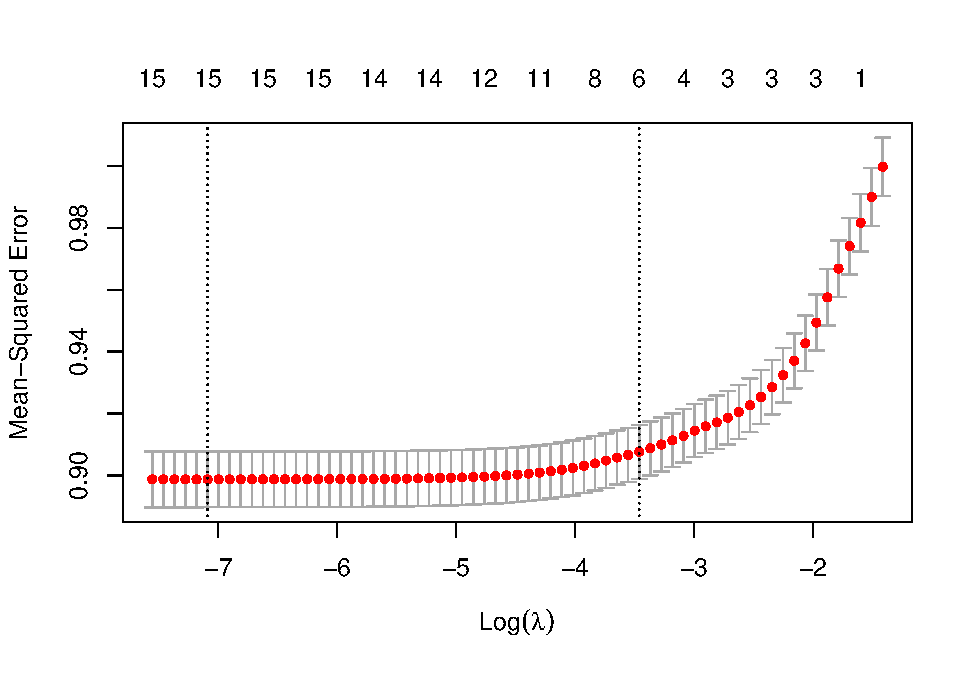
\includegraphics{../results/report_files/figure-latex/BB-lasso-plot-1.pdf}

\begin{Shaded}
\begin{Highlighting}[]
\FunctionTok{coef}\NormalTok{(BB.glmnet.cv, }\FunctionTok{c}\NormalTok{(BB.glmnet.cv}\SpecialCharTok{$}\NormalTok{lambda.min,}
\NormalTok{                   BB.glmnet.cv}\SpecialCharTok{$}\NormalTok{lambda}\FloatTok{.1}\NormalTok{se))}
\end{Highlighting}
\end{Shaded}

\begin{verbatim}
## 17 x 2 sparse Matrix of class "dgCMatrix"
##                                    s1            s2
## (Intercept)             -2.424344e-16 -1.012851e-16
## SID                      1.982979e-03  .           
## SexMale                  2.395217e-02  .           
## Age                     -5.080671e-02  .           
## packyrs                  3.581281e-02  4.173688e-03
## alcoholintakegpd         3.411826e-03  .           
## PriorMed                 1.750507e-02  .           
## HypertensionTRUE         3.782778e-02  1.019900e-02
## ObesityTRUE             -1.044448e-02  .           
## `Diabetes Mellitus`TRUE  2.086409e-02  .           
## CADTRUE                  7.322854e-03  .           
## HypercholTRUE           -7.898300e-03  .           
## `Heart Failure`TRUE      .             .           
## bmi                     -8.685689e-02 -3.159110e-02
## sbp                      1.572566e-01  1.167419e-01
## dbp                      1.233614e-01  1.224064e-01
## pulse_rate               1.682552e-01  1.278304e-01
\end{verbatim}

\hypertarget{acei}{%
\subsection{ACEi}\label{acei}}

\begin{Shaded}
\begin{Highlighting}[]
\NormalTok{ACEi.df }\OtherTok{\textless{}{-}}\NormalTok{ dfs }\SpecialCharTok{\%\textgreater{}\%} 
  \FunctionTok{filter}\NormalTok{(Drug}\SpecialCharTok{==}\StringTok{"ACEi"}\NormalTok{) }\SpecialCharTok{\%\textgreater{}\%} 
  \FunctionTok{select}\NormalTok{(}\SpecialCharTok{{-}}\NormalTok{Drug)}
\end{Highlighting}
\end{Shaded}

\begin{Shaded}
\begin{Highlighting}[]
\NormalTok{ACEi.fits.df }\OtherTok{\textless{}{-}}\NormalTok{ fits.df }\SpecialCharTok{\%\textgreater{}\%} 
  \FunctionTok{filter}\NormalTok{(Drug}\SpecialCharTok{==}\StringTok{"ACEi"}\NormalTok{)}
\end{Highlighting}
\end{Shaded}

\begin{Shaded}
\begin{Highlighting}[]
\FunctionTok{get\_pretty\_fit\_table}\NormalTok{(ACEi.fits.df, }\StringTok{"ACEi"}\NormalTok{)}
\end{Highlighting}
\end{Shaded}

\begin{table}

\caption{\label{tab:ACEi-fit-table}ACEi: Coefficients from linear models}
\centering
\begin{tabular}[t]{l|r|r|r|r|r|r|l}
\hline
term & estimate & std.error & statistic & p.value & conf.low & conf.high & Adjustment\\
\hline
(Intercept) & -20.514 & 0.517 & -39.675 & 0.000 & -21.527 & -19.501 & With SBP/DBP/HR\\
\hline
(Intercept) & -0.867 & 0.359 & -2.415 & 0.016 & -1.571 & -0.164 & Without SBP/DBP/HR\\
\hline
`Diabetes Mellitus`TRUE & 0.667 & 0.177 & 3.780 & 0.000 & 0.321 & 1.013 & With SBP/DBP/HR\\
\hline
`Diabetes Mellitus`TRUE & 0.629 & 0.184 & 3.428 & 0.001 & 0.269 & 0.989 & Without SBP/DBP/HR\\
\hline
`Heart Failure`TRUE & 0.112 & 0.371 & 0.303 & 0.762 & -0.615 & 0.839 & With SBP/DBP/HR\\
\hline
`Heart Failure`TRUE & -0.069 & 0.388 & -0.178 & 0.858 & -0.830 & 0.691 & Without SBP/DBP/HR\\
\hline
alcoholintakegpd & 0.001 & 0.003 & 0.328 & 0.743 & -0.004 & 0.006 & With SBP/DBP/HR\\
\hline
alcoholintakegpd & 0.006 & 0.003 & 2.344 & 0.019 & 0.001 & 0.011 & Without SBP/DBP/HR\\
\hline
bmi & -0.147 & 0.014 & -10.520 & 0.000 & -0.174 & -0.119 & With SBP/DBP/HR\\
\hline
bmi & -0.001 & 0.014 & -0.064 & 0.949 & -0.029 & 0.027 & Without SBP/DBP/HR\\
\hline
CADTRUE & 0.463 & 0.178 & 2.600 & 0.009 & 0.114 & 0.812 & With SBP/DBP/HR\\
\hline
CADTRUE & -0.423 & 0.185 & -2.284 & 0.022 & -0.785 & -0.060 & Without SBP/DBP/HR\\
\hline
dbp & 0.087 & 0.006 & 13.980 & 0.000 & 0.075 & 0.099 & With SBP/DBP/HR\\
\hline
HypercholTRUE & -0.139 & 0.112 & -1.242 & 0.214 & -0.358 & 0.080 & With SBP/DBP/HR\\
\hline
HypercholTRUE & -0.215 & 0.117 & -1.838 & 0.066 & -0.444 & 0.014 & Without SBP/DBP/HR\\
\hline
HypertensionTRUE & 0.663 & 0.107 & 6.226 & 0.000 & 0.454 & 0.872 & With SBP/DBP/HR\\
\hline
HypertensionTRUE & 1.894 & 0.108 & 17.524 & 0.000 & 1.682 & 2.106 & Without SBP/DBP/HR\\
\hline
ObesityTRUE & -0.257 & 0.148 & -1.732 & 0.083 & -0.547 & 0.034 & With SBP/DBP/HR\\
\hline
ObesityTRUE & -0.733 & 0.155 & -4.739 & 0.000 & -1.037 & -0.430 & Without SBP/DBP/HR\\
\hline
packyrs & 0.023 & 0.004 & 6.049 & 0.000 & 0.015 & 0.030 & With SBP/DBP/HR\\
\hline
packyrs & 0.022 & 0.004 & 5.473 & 0.000 & 0.014 & 0.029 & Without SBP/DBP/HR\\
\hline
poly(Age, 2)1 & -68.774 & 8.357 & -8.230 & 0.000 & -85.154 & -52.394 & With SBP/DBP/HR\\
\hline
poly(Age, 2)1 & -24.893 & 7.937 & -3.136 & 0.002 & -40.449 & -9.336 & Without SBP/DBP/HR\\
\hline
poly(Age, 2)2 & -106.492 & 7.248 & -14.693 & 0.000 & -120.698 & -92.286 & With SBP/DBP/HR\\
\hline
poly(Age, 2)2 & -113.511 & 7.563 & -15.008 & 0.000 & -128.336 & -98.687 & Without SBP/DBP/HR\\
\hline
PriorMed & -0.044 & 0.168 & -0.260 & 0.795 & -0.373 & 0.286 & With SBP/DBP/HR\\
\hline
PriorMed & -0.420 & 0.176 & -2.390 & 0.017 & -0.764 & -0.075 & Without SBP/DBP/HR\\
\hline
pulse\_rate & 0.110 & 0.004 & 27.843 & 0.000 & 0.102 & 0.118 & With SBP/DBP/HR\\
\hline
sbp & 0.067 & 0.003 & 19.621 & 0.000 & 0.061 & 0.074 & With SBP/DBP/HR\\
\hline
SexMale & 0.452 & 0.095 & 4.766 & 0.000 & 0.266 & 0.637 & With SBP/DBP/HR\\
\hline
SexMale & 0.533 & 0.096 & 5.551 & 0.000 & 0.345 & 0.722 & Without SBP/DBP/HR\\
\hline
\end{tabular}
\end{table}

\begin{Shaded}
\begin{Highlighting}[]
\FunctionTok{get\_pretty\_fit\_forest\_plot}\NormalTok{(ACEi.fits.df) }\OtherTok{{-}\textgreater{}}\NormalTok{p}
\NormalTok{p}
\end{Highlighting}
\end{Shaded}

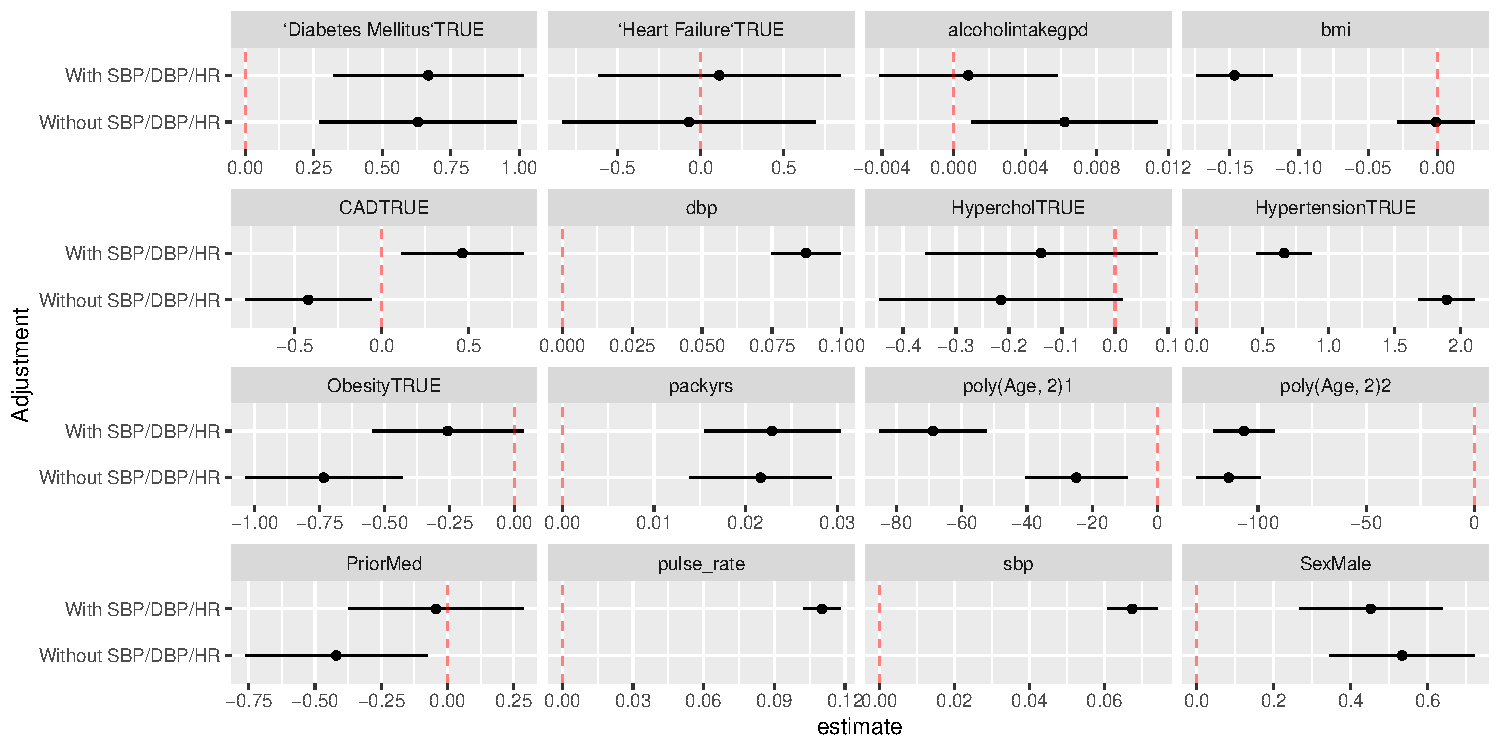
\includegraphics{../results/report_files/figure-latex/ACEi-fit-forest-1.pdf}

\begin{Shaded}
\begin{Highlighting}[]
\NormalTok{ACEi.fits.df }\SpecialCharTok{\%\textgreater{}\%} 
\NormalTok{  get\_fit\_glance}
\end{Highlighting}
\end{Shaded}

\begin{verbatim}
## # A tibble: 2 x 5
##   AdditionalMarkers     N fracPriorMed adj.r.squared r.squared
##   <lgl>             <dbl>        <dbl>         <dbl>     <dbl>
## 1 FALSE             27546        0.088         0.024     0.024
## 2 TRUE              27546        0.088         0.108     0.109
\end{verbatim}

\begin{Shaded}
\begin{Highlighting}[]
\FunctionTok{generate\_table.self.reported}\NormalTok{(ACEi.df, }\StringTok{"ACEi"}\NormalTok{)}
\end{Highlighting}
\end{Shaded}

\begin{verbatim}
## Table printed with `knitr::kable()`, not {gt}. Learn why at
## https://www.danieldsjoberg.com/gtsummary/articles/rmarkdown.html
## To suppress this message, include `message = FALSE` in code chunk header.
\end{verbatim}

\begin{tabular}{l|c|c|c}
\hline
**Characteristic** & **ACEi**, N = 2,412 & **No ACEi**, N = 25,134 & **p-value**\\
\hline
Cardiac Age gap & 0.7 (-4.6, 5.9) & 0.1 (-5.4, 5.3) & <0.001\\
\hline
Sex &  &  & <0.001\\
\hline
Female & 764 (32\%) & 13,073 (52\%) & \\
\hline
Male & 1,648 (68\%) & 12,061 (48\%) & \\
\hline
Age & 67 (61, 71) & 64 (58, 70) & <0.001\\
\hline
Packs year of smoking & 0 (0, 7) & 0 (0, 3) & <0.001\\
\hline
Alcohol is g/day consumed & 4 (0, 18) & 4 (0, 15) & 0.004\\
\hline
Hypertension & 2,075 (86\%) & 7,123 (28\%) & <0.001\\
\hline
Obesity & 776 (32\%) & 4,899 (19\%) & <0.001\\
\hline
Diabetes Mellitus & 446 (18\%) & 1,537 (6.1\%) & <0.001\\
\hline
Coronary Artery Disease & 621 (26\%) & 1,487 (5.9\%) & <0.001\\
\hline
Hypercholesterolemia & 1,086 (45\%) & 5,205 (21\%) & <0.001\\
\hline
Heart Failure & 145 (6.0\%) & 267 (1.1\%) & <0.001\\
\hline
dbp & 80 (72, 86) & 78 (72, 85) & <0.001\\
\hline
sbp & 142 (131, 154) & 137 (126, 150) & <0.001\\
\hline
pulse\_rate & 68 (60, 76) & 68 (61, 76) & 0.6\\
\hline
bmi & 27.9 (25.1, 30.9) & 26.1 (23.7, 29.1) & <0.001\\
\hline
\end{tabular}

\begin{Shaded}
\begin{Highlighting}[]
\NormalTok{ACEi.df }\SpecialCharTok{\%\textgreater{}\%} 
  \FunctionTok{get\_stratified\_age\_gap\_histogram}\NormalTok{(}\StringTok{"ACEi"}\NormalTok{)}
\end{Highlighting}
\end{Shaded}

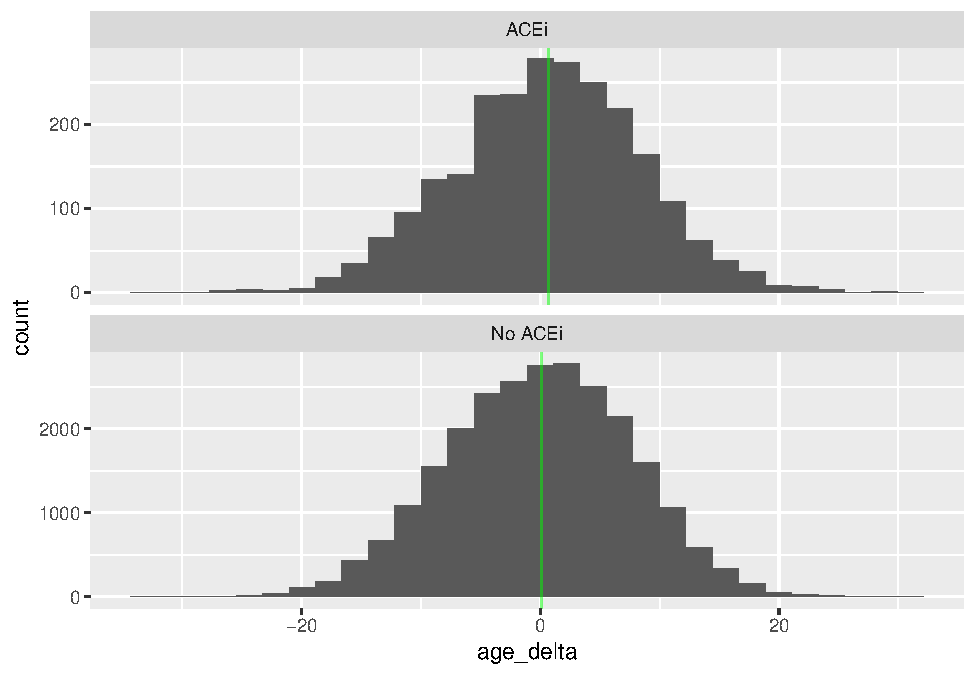
\includegraphics{../results/report_files/figure-latex/ACEi-age-gap-histograms-1.pdf}

\begin{Shaded}
\begin{Highlighting}[]
\NormalTok{ACEi.df }\SpecialCharTok{\%\textgreater{}\%} 
   \FunctionTok{get\_stratified\_age\_gap\_quantiles}\NormalTok{(}\StringTok{"ACEi"}\NormalTok{)}
\end{Highlighting}
\end{Shaded}

\begin{verbatim}
## # A tibble: 2 x 9
##   PriorMed  `1%` `2.5%` `25%` `50%` `75%` `97.5%` `99%`     N
##   <chr>    <dbl>  <dbl> <dbl> <dbl> <dbl>   <dbl> <dbl> <int>
## 1 ACEi     -17.6  -14.6 -4.55  0.71  5.89    15.6  18.2  2412
## 2 No ACEi  -17.7  -15.1 -5.38  0.12  5.28    14.2  16.7 25134
\end{verbatim}

\hypertarget{lasso-4}{%
\subsubsection{Lasso}\label{lasso-4}}

\begin{Shaded}
\begin{Highlighting}[]
\NormalTok{ACEi.glmnet.cv }\OtherTok{\textless{}{-}}\NormalTok{ fits.glm[[}\StringTok{"ACEi"}\NormalTok{]]}
\end{Highlighting}
\end{Shaded}

\begin{Shaded}
\begin{Highlighting}[]
\FunctionTok{plot}\NormalTok{(ACEi.glmnet.cv) }
\end{Highlighting}
\end{Shaded}

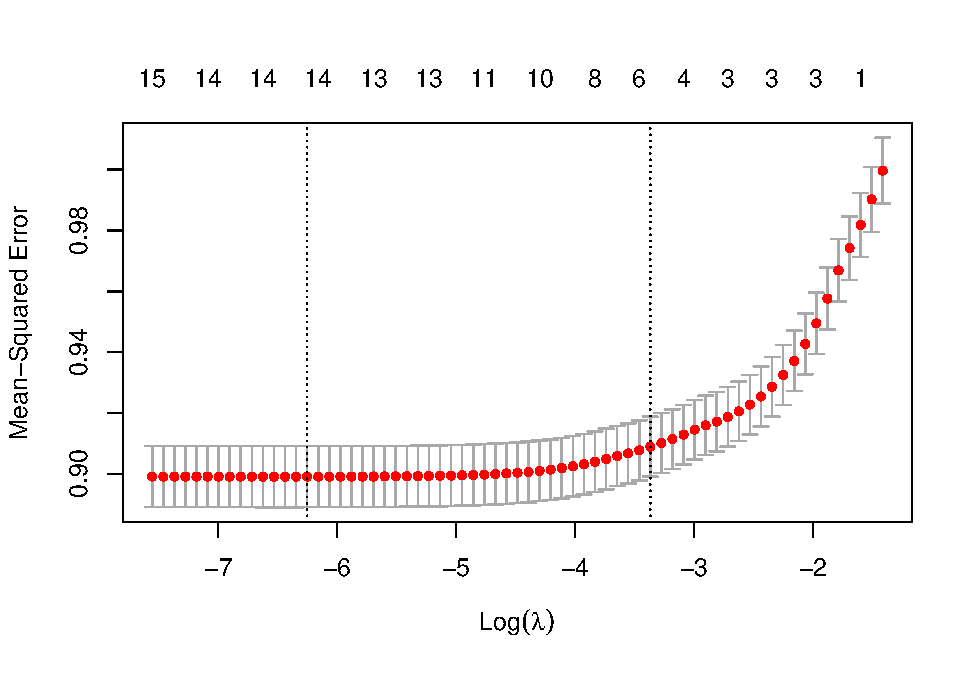
\includegraphics{../results/report_files/figure-latex/ACEi-lasso-plot-1.pdf}

\begin{Shaded}
\begin{Highlighting}[]
\FunctionTok{coef}\NormalTok{(ACEi.glmnet.cv, }\FunctionTok{c}\NormalTok{(ACEi.glmnet.cv}\SpecialCharTok{$}\NormalTok{lambda.min,}
\NormalTok{                   ACEi.glmnet.cv}\SpecialCharTok{$}\NormalTok{lambda}\FloatTok{.1}\NormalTok{se))}
\end{Highlighting}
\end{Shaded}

\begin{verbatim}
## 17 x 2 sparse Matrix of class "dgCMatrix"
##                                    s1            s2
## (Intercept)             -2.286956e-16 -9.385681e-17
## SID                      8.920302e-04  .           
## SexMale                  2.276959e-02  .           
## Age                     -4.767750e-02  .           
## packyrs                  3.479136e-02  8.410991e-04
## alcoholintakegpd         2.885660e-03  .           
## PriorMed                 .             .           
## HypertensionTRUE         3.907782e-02  7.401584e-03
## ObesityTRUE             -9.937072e-03  .           
## `Diabetes Mellitus`TRUE  2.011325e-02  .           
## CADTRUE                  1.147156e-02  .           
## HypercholTRUE           -5.361039e-03  .           
## `Heart Failure`TRUE      .             .           
## bmi                     -8.367754e-02 -2.634601e-02
## sbp                      1.545082e-01  1.151769e-01
## dbp                      1.233096e-01  1.201523e-01
## pulse_rate               1.643223e-01  1.247856e-01
\end{verbatim}

\hypertarget{arb}{%
\subsection{ARB}\label{arb}}

\begin{Shaded}
\begin{Highlighting}[]
\NormalTok{ARB.df }\OtherTok{\textless{}{-}}\NormalTok{ dfs }\SpecialCharTok{\%\textgreater{}\%} 
  \FunctionTok{filter}\NormalTok{(Drug}\SpecialCharTok{==}\StringTok{"ARB"}\NormalTok{) }\SpecialCharTok{\%\textgreater{}\%} 
  \FunctionTok{select}\NormalTok{(}\SpecialCharTok{{-}}\NormalTok{Drug)}
\end{Highlighting}
\end{Shaded}

\begin{Shaded}
\begin{Highlighting}[]
\NormalTok{ARB.fits.df }\OtherTok{\textless{}{-}}\NormalTok{ fits.df }\SpecialCharTok{\%\textgreater{}\%} 
  \FunctionTok{filter}\NormalTok{(Drug}\SpecialCharTok{==}\StringTok{"ARB"}\NormalTok{)}
\end{Highlighting}
\end{Shaded}

\begin{Shaded}
\begin{Highlighting}[]
\FunctionTok{get\_pretty\_fit\_table}\NormalTok{(ARB.fits.df, }\StringTok{"ARB"}\NormalTok{)}
\end{Highlighting}
\end{Shaded}

\begin{table}

\caption{\label{tab:ARB-fit-table}ARB: Coefficients from linear models}
\centering
\begin{tabular}[t]{l|r|r|r|r|r|r|l}
\hline
term & estimate & std.error & statistic & p.value & conf.low & conf.high & Adjustment\\
\hline
(Intercept) & -20.512 & 0.517 & -39.681 & 0.000 & -21.525 & -19.498 & With SBP/DBP/HR\\
\hline
(Intercept) & -0.862 & 0.359 & -2.397 & 0.017 & -1.566 & -0.157 & Without SBP/DBP/HR\\
\hline
`Diabetes Mellitus`TRUE & 0.656 & 0.177 & 3.718 & 0.000 & 0.310 & 1.002 & With SBP/DBP/HR\\
\hline
`Diabetes Mellitus`TRUE & 0.607 & 0.184 & 3.309 & 0.001 & 0.248 & 0.967 & Without SBP/DBP/HR\\
\hline
`Heart Failure`TRUE & 0.099 & 0.370 & 0.267 & 0.789 & -0.627 & 0.825 & With SBP/DBP/HR\\
\hline
`Heart Failure`TRUE & -0.123 & 0.388 & -0.317 & 0.751 & -0.882 & 0.637 & Without SBP/DBP/HR\\
\hline
alcoholintakegpd & 0.001 & 0.003 & 0.325 & 0.745 & -0.004 & 0.006 & With SBP/DBP/HR\\
\hline
alcoholintakegpd & 0.006 & 0.003 & 2.333 & 0.020 & 0.001 & 0.011 & Without SBP/DBP/HR\\
\hline
bmi & -0.147 & 0.014 & -10.559 & 0.000 & -0.175 & -0.120 & With SBP/DBP/HR\\
\hline
bmi & -0.001 & 0.014 & -0.062 & 0.951 & -0.029 & 0.027 & Without SBP/DBP/HR\\
\hline
CADTRUE & 0.450 & 0.176 & 2.550 & 0.011 & 0.104 & 0.796 & With SBP/DBP/HR\\
\hline
CADTRUE & -0.483 & 0.183 & -2.632 & 0.008 & -0.842 & -0.123 & Without SBP/DBP/HR\\
\hline
dbp & 0.087 & 0.006 & 14.004 & 0.000 & 0.075 & 0.100 & With SBP/DBP/HR\\
\hline
HypercholTRUE & -0.143 & 0.112 & -1.275 & 0.202 & -0.362 & 0.077 & With SBP/DBP/HR\\
\hline
HypercholTRUE & -0.226 & 0.117 & -1.934 & 0.053 & -0.455 & 0.003 & Without SBP/DBP/HR\\
\hline
HypertensionTRUE & 0.628 & 0.106 & 5.942 & 0.000 & 0.421 & 0.836 & With SBP/DBP/HR\\
\hline
HypertensionTRUE & 1.827 & 0.107 & 17.005 & 0.000 & 1.616 & 2.037 & Without SBP/DBP/HR\\
\hline
ObesityTRUE & -0.255 & 0.148 & -1.723 & 0.085 & -0.546 & 0.035 & With SBP/DBP/HR\\
\hline
ObesityTRUE & -0.738 & 0.155 & -4.770 & 0.000 & -1.041 & -0.435 & Without SBP/DBP/HR\\
\hline
packyrs & 0.023 & 0.004 & 6.059 & 0.000 & 0.016 & 0.030 & With SBP/DBP/HR\\
\hline
packyrs & 0.022 & 0.004 & 5.456 & 0.000 & 0.014 & 0.029 & Without SBP/DBP/HR\\
\hline
poly(Age, 2)1 & -68.999 & 8.360 & -8.253 & 0.000 & -85.386 & -52.612 & With SBP/DBP/HR\\
\hline
poly(Age, 2)1 & -24.507 & 7.942 & -3.086 & 0.002 & -40.073 & -8.940 & Without SBP/DBP/HR\\
\hline
poly(Age, 2)2 & -106.467 & 7.247 & -14.692 & 0.000 & -120.671 & -92.263 & With SBP/DBP/HR\\
\hline
poly(Age, 2)2 & -113.256 & 7.563 & -14.974 & 0.000 & -128.080 & -98.431 & Without SBP/DBP/HR\\
\hline
PriorMed & 0.183 & 0.195 & 0.937 & 0.349 & -0.200 & 0.565 & With SBP/DBP/HR\\
\hline
PriorMed & -0.059 & 0.204 & -0.289 & 0.772 & -0.459 & 0.341 & Without SBP/DBP/HR\\
\hline
pulse\_rate & 0.110 & 0.004 & 27.848 & 0.000 & 0.103 & 0.118 & With SBP/DBP/HR\\
\hline
sbp & 0.067 & 0.003 & 19.632 & 0.000 & 0.061 & 0.074 & With SBP/DBP/HR\\
\hline
SexMale & 0.452 & 0.095 & 4.772 & 0.000 & 0.266 & 0.637 & With SBP/DBP/HR\\
\hline
SexMale & 0.521 & 0.096 & 5.432 & 0.000 & 0.333 & 0.710 & Without SBP/DBP/HR\\
\hline
\end{tabular}
\end{table}

\begin{Shaded}
\begin{Highlighting}[]
\FunctionTok{get\_pretty\_fit\_forest\_plot}\NormalTok{(ARB.fits.df) }\OtherTok{{-}\textgreater{}}\NormalTok{p}
\NormalTok{p}
\end{Highlighting}
\end{Shaded}

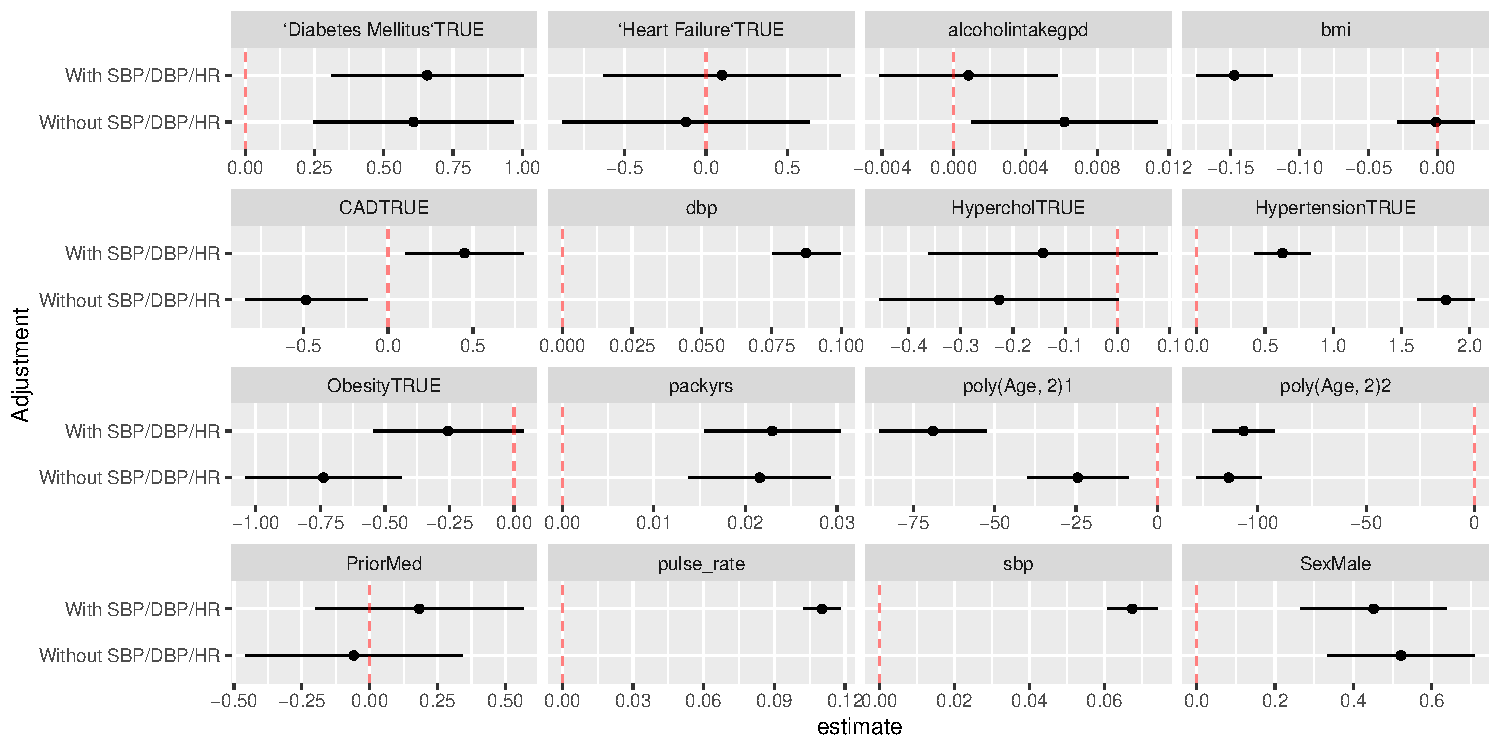
\includegraphics{../results/report_files/figure-latex/ARB-fit-forest-1.pdf}

\begin{Shaded}
\begin{Highlighting}[]
\NormalTok{ARB.fits.df }\SpecialCharTok{\%\textgreater{}\%} 
\NormalTok{  get\_fit\_glance}
\end{Highlighting}
\end{Shaded}

\begin{verbatim}
## # A tibble: 2 x 5
##   AdditionalMarkers     N fracPriorMed adj.r.squared r.squared
##   <lgl>             <dbl>        <dbl>         <dbl>     <dbl>
## 1 FALSE             27546         0.06         0.024     0.024
## 2 TRUE              27546         0.06         0.108     0.109
\end{verbatim}

\begin{Shaded}
\begin{Highlighting}[]
\FunctionTok{generate\_table.self.reported}\NormalTok{(ARB.df, }\StringTok{"ARB"}\NormalTok{)}
\end{Highlighting}
\end{Shaded}

\begin{verbatim}
## Table printed with `knitr::kable()`, not {gt}. Learn why at
## https://www.danieldsjoberg.com/gtsummary/articles/rmarkdown.html
## To suppress this message, include `message = FALSE` in code chunk header.
\end{verbatim}

\begin{tabular}{l|c|c|c}
\hline
**Characteristic** & **ARB**, N = 1,642 & **No ARB**, N = 25,904 & **p-value**\\
\hline
Cardiac Age gap & 1.2 (-4.1, 6.3) & 0.1 (-5.4, 5.3) & <0.001\\
\hline
Sex &  &  & <0.001\\
\hline
Female & 712 (43\%) & 13,125 (51\%) & \\
\hline
Male & 930 (57\%) & 12,779 (49\%) & \\
\hline
Age & 68 (62, 72) & 64 (58, 70) & <0.001\\
\hline
Packs year of smoking & 0 (0, 4) & 0 (0, 3) & 0.4\\
\hline
Alcohol is g/day consumed & 4 (0, 18) & 4 (0, 15) & 0.063\\
\hline
Hypertension & 1,535 (93\%) & 7,663 (30\%) & <0.001\\
\hline
Obesity & 568 (35\%) & 5,107 (20\%) & <0.001\\
\hline
Diabetes Mellitus & 315 (19\%) & 1,668 (6.4\%) & <0.001\\
\hline
Coronary Artery Disease & 295 (18\%) & 1,813 (7.0\%) & <0.001\\
\hline
Hypercholesterolemia & 708 (43\%) & 5,583 (22\%) & <0.001\\
\hline
Heart Failure & 67 (4.1\%) & 345 (1.3\%) & <0.001\\
\hline
dbp & 80 (74, 87) & 78 (72, 85) & <0.001\\
\hline
sbp & 144 (134, 156) & 137 (126, 150) & <0.001\\
\hline
pulse\_rate & 69 (62, 78) & 68 (60, 76) & <0.001\\
\hline
bmi & 28.3 (25.9, 31.4) & 26.1 (23.7, 29.1) & <0.001\\
\hline
\end{tabular}

\begin{Shaded}
\begin{Highlighting}[]
\NormalTok{ARB.df }\SpecialCharTok{\%\textgreater{}\%} 
  \FunctionTok{get\_stratified\_age\_gap\_histogram}\NormalTok{(}\StringTok{"ARB"}\NormalTok{)}
\end{Highlighting}
\end{Shaded}

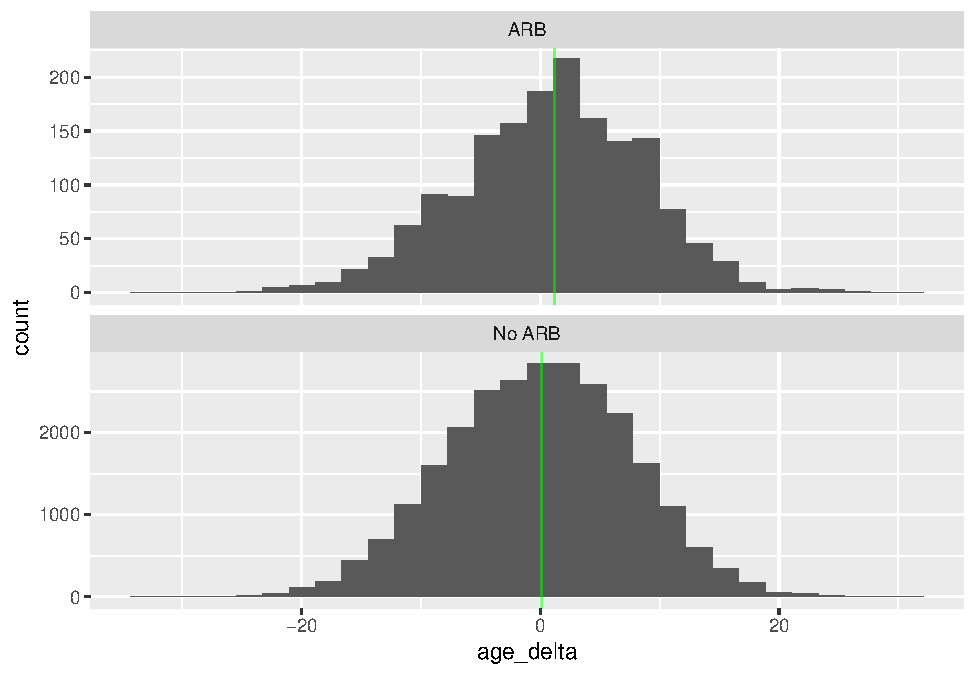
\includegraphics{../results/report_files/figure-latex/ARB-age-gap-histograms-1.pdf}

\begin{Shaded}
\begin{Highlighting}[]
\NormalTok{ARB.df }\SpecialCharTok{\%\textgreater{}\%} 
    \FunctionTok{get\_stratified\_age\_gap\_quantiles}\NormalTok{(}\StringTok{"ARB"}\NormalTok{)}
\end{Highlighting}
\end{Shaded}

\begin{verbatim}
## # A tibble: 2 x 9
##   PriorMed  `1%` `2.5%` `25%` `50%` `75%` `97.5%` `99%`     N
##   <chr>    <dbl>  <dbl> <dbl> <dbl> <dbl>   <dbl> <dbl> <int>
## 1 ARB      -18.0  -14.8 -4.1   1.19  6.29    14.9  17.2  1642
## 2 No ARB   -17.7  -15.0 -5.37  0.09  5.28    14.3  16.9 25904
\end{verbatim}

\hypertarget{lasso-5}{%
\subsubsection{Lasso}\label{lasso-5}}

\begin{Shaded}
\begin{Highlighting}[]
\NormalTok{ARB.glmnet.cv }\OtherTok{\textless{}{-}}\NormalTok{ fits.glm[[}\StringTok{"ARB"}\NormalTok{]]}
\end{Highlighting}
\end{Shaded}

\begin{Shaded}
\begin{Highlighting}[]
\FunctionTok{plot}\NormalTok{(ARB.glmnet.cv) }
\end{Highlighting}
\end{Shaded}

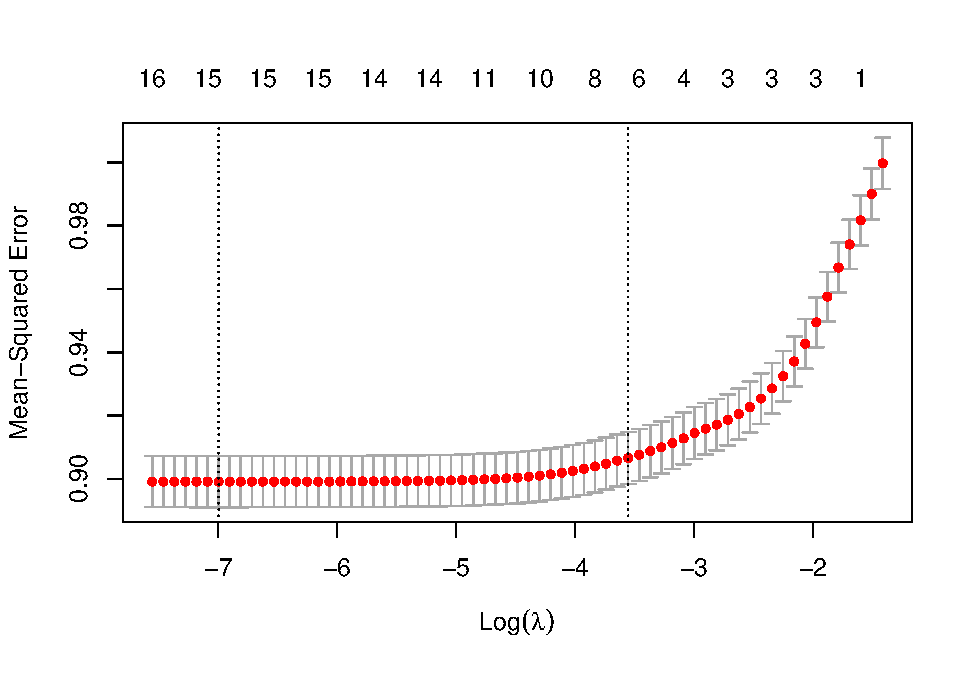
\includegraphics{../results/report_files/figure-latex/ARB-lasso-plot-1.pdf}

\begin{Shaded}
\begin{Highlighting}[]
\FunctionTok{coef}\NormalTok{(ARB.glmnet.cv, }\FunctionTok{c}\NormalTok{(ARB.glmnet.cv}\SpecialCharTok{$}\NormalTok{lambda.min,}
\NormalTok{                   ARB.glmnet.cv}\SpecialCharTok{$}\NormalTok{lambda}\FloatTok{.1}\NormalTok{se))}
\end{Highlighting}
\end{Shaded}

\begin{verbatim}
## 17 x 2 sparse Matrix of class "dgCMatrix"
##                                    s1            s2
## (Intercept)             -2.314783e-16 -1.080653e-16
## SID                      1.962549e-03  .           
## SexMale                  2.374022e-02  .           
## Age                     -4.971222e-02  .           
## packyrs                  3.580341e-02  7.207680e-03
## alcoholintakegpd         3.515135e-03  .           
## PriorMed                 4.828414e-03  .           
## HypertensionTRUE         3.879835e-02  1.273594e-02
## ObesityTRUE             -1.039479e-02  .           
## `Diabetes Mellitus`TRUE  2.102259e-02  .           
## CADTRUE                  1.259680e-02  .           
## HypercholTRUE           -7.020339e-03  .           
## `Heart Failure`TRUE      .             .           
## bmi                     -8.573188e-02 -3.636707e-02
## sbp                      1.559629e-01  1.182037e-01
## dbp                      1.233456e-01  1.244400e-01
## pulse_rate               1.657049e-01  1.306085e-01
\end{verbatim}

\hypertarget{ccb}{%
\subsection{CCB}\label{ccb}}

\begin{Shaded}
\begin{Highlighting}[]
\NormalTok{CCB.df }\OtherTok{\textless{}{-}}\NormalTok{ dfs }\SpecialCharTok{\%\textgreater{}\%} 
  \FunctionTok{filter}\NormalTok{(Drug}\SpecialCharTok{==}\StringTok{"CCB"}\NormalTok{) }\SpecialCharTok{\%\textgreater{}\%} 
  \FunctionTok{select}\NormalTok{(}\SpecialCharTok{{-}}\NormalTok{Drug)}
\end{Highlighting}
\end{Shaded}

\begin{Shaded}
\begin{Highlighting}[]
\NormalTok{CCB.fits.df }\OtherTok{\textless{}{-}}\NormalTok{ fits.df }\SpecialCharTok{\%\textgreater{}\%} 
  \FunctionTok{filter}\NormalTok{(Drug}\SpecialCharTok{==}\StringTok{"CCB"}\NormalTok{)}
\end{Highlighting}
\end{Shaded}

\begin{Shaded}
\begin{Highlighting}[]
\FunctionTok{get\_pretty\_fit\_table}\NormalTok{(CCB.fits.df, }\StringTok{"CCB"}\NormalTok{)}
\end{Highlighting}
\end{Shaded}

\begin{table}

\caption{\label{tab:CCB-fit-table}CCB: Coefficients from linear models}
\centering
\begin{tabular}[t]{l|r|r|r|r|r|r|l}
\hline
term & estimate & std.error & statistic & p.value & conf.low & conf.high & Adjustment\\
\hline
(Intercept) & -20.491 & 0.517 & -39.635 & 0.000 & -21.505 & -19.478 & With SBP/DBP/HR\\
\hline
(Intercept) & -0.871 & 0.359 & -2.427 & 0.015 & -1.575 & -0.168 & Without SBP/DBP/HR\\
\hline
`Diabetes Mellitus`TRUE & 0.668 & 0.176 & 3.786 & 0.000 & 0.322 & 1.013 & With SBP/DBP/HR\\
\hline
`Diabetes Mellitus`TRUE & 0.616 & 0.183 & 3.359 & 0.001 & 0.256 & 0.975 & Without SBP/DBP/HR\\
\hline
`Heart Failure`TRUE & 0.090 & 0.370 & 0.242 & 0.808 & -0.636 & 0.816 & With SBP/DBP/HR\\
\hline
`Heart Failure`TRUE & -0.158 & 0.387 & -0.407 & 0.684 & -0.917 & 0.602 & Without SBP/DBP/HR\\
\hline
alcoholintakegpd & 0.001 & 0.003 & 0.356 & 0.722 & -0.004 & 0.006 & With SBP/DBP/HR\\
\hline
alcoholintakegpd & 0.006 & 0.003 & 2.383 & 0.017 & 0.001 & 0.011 & Without SBP/DBP/HR\\
\hline
bmi & -0.146 & 0.014 & -10.485 & 0.000 & -0.173 & -0.119 & With SBP/DBP/HR\\
\hline
bmi & -0.001 & 0.014 & -0.043 & 0.965 & -0.029 & 0.027 & Without SBP/DBP/HR\\
\hline
CADTRUE & 0.450 & 0.176 & 2.553 & 0.011 & 0.105 & 0.796 & With SBP/DBP/HR\\
\hline
CADTRUE & -0.496 & 0.183 & -2.704 & 0.007 & -0.855 & -0.136 & Without SBP/DBP/HR\\
\hline
dbp & 0.087 & 0.006 & 13.866 & 0.000 & 0.074 & 0.099 & With SBP/DBP/HR\\
\hline
HypercholTRUE & -0.137 & 0.112 & -1.225 & 0.221 & -0.356 & 0.082 & With SBP/DBP/HR\\
\hline
HypercholTRUE & -0.219 & 0.117 & -1.873 & 0.061 & -0.448 & 0.010 & Without SBP/DBP/HR\\
\hline
HypertensionTRUE & 0.749 & 0.111 & 6.726 & 0.000 & 0.531 & 0.967 & With SBP/DBP/HR\\
\hline
HypertensionTRUE & 2.003 & 0.113 & 17.738 & 0.000 & 1.781 & 2.224 & Without SBP/DBP/HR\\
\hline
ObesityTRUE & -0.259 & 0.148 & -1.750 & 0.080 & -0.550 & 0.031 & With SBP/DBP/HR\\
\hline
ObesityTRUE & -0.740 & 0.155 & -4.782 & 0.000 & -1.043 & -0.437 & Without SBP/DBP/HR\\
\hline
packyrs & 0.023 & 0.004 & 6.040 & 0.000 & 0.015 & 0.030 & With SBP/DBP/HR\\
\hline
packyrs & 0.022 & 0.004 & 5.461 & 0.000 & 0.014 & 0.029 & Without SBP/DBP/HR\\
\hline
poly(Age, 2)1 & -67.735 & 8.370 & -8.092 & 0.000 & -84.141 & -51.329 & With SBP/DBP/HR\\
\hline
poly(Age, 2)1 & -22.451 & 7.952 & -2.823 & 0.005 & -38.037 & -6.865 & Without SBP/DBP/HR\\
\hline
poly(Age, 2)2 & -106.555 & 7.247 & -14.704 & 0.000 & -120.759 & -92.352 & With SBP/DBP/HR\\
\hline
poly(Age, 2)2 & -113.337 & 7.561 & -14.989 & 0.000 & -128.157 & -98.517 & Without SBP/DBP/HR\\
\hline
PriorMed & -0.337 & 0.162 & -2.079 & 0.038 & -0.655 & -0.019 & With SBP/DBP/HR\\
\hline
PriorMed & -0.685 & 0.169 & -4.051 & 0.000 & -1.017 & -0.354 & Without SBP/DBP/HR\\
\hline
pulse\_rate & 0.111 & 0.004 & 27.901 & 0.000 & 0.103 & 0.118 & With SBP/DBP/HR\\
\hline
sbp & 0.067 & 0.003 & 19.609 & 0.000 & 0.061 & 0.074 & With SBP/DBP/HR\\
\hline
SexMale & 0.461 & 0.095 & 4.863 & 0.000 & 0.275 & 0.647 & With SBP/DBP/HR\\
\hline
SexMale & 0.536 & 0.096 & 5.587 & 0.000 & 0.348 & 0.725 & Without SBP/DBP/HR\\
\hline
\end{tabular}
\end{table}

\begin{Shaded}
\begin{Highlighting}[]
\FunctionTok{get\_pretty\_fit\_forest\_plot}\NormalTok{(CCB.fits.df) }\OtherTok{{-}\textgreater{}}\NormalTok{p}
\NormalTok{p}
\end{Highlighting}
\end{Shaded}

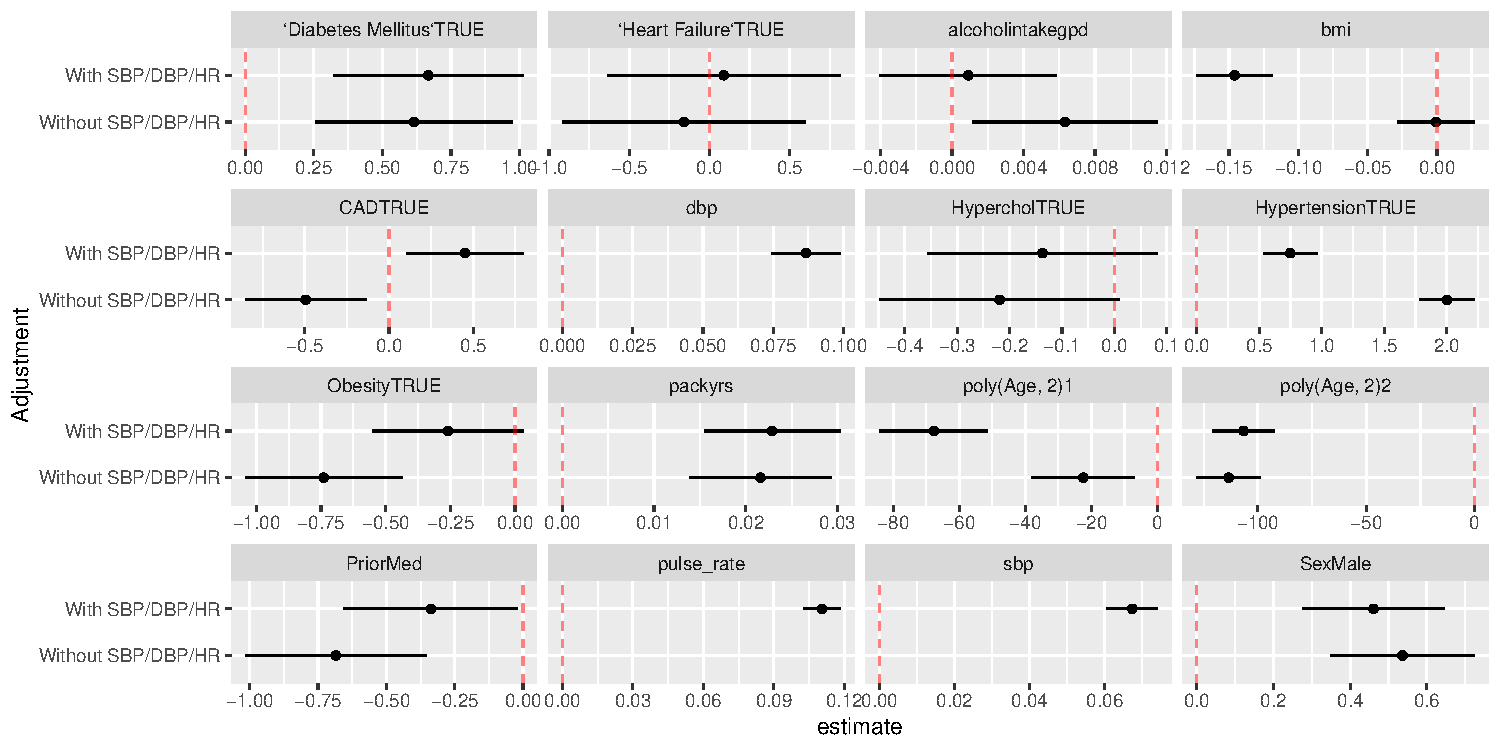
\includegraphics{../results/report_files/figure-latex/CCB-fit-forest-1.pdf}

\begin{Shaded}
\begin{Highlighting}[]
\NormalTok{CCB.fits.df }\SpecialCharTok{\%\textgreater{}\%} 
\NormalTok{  get\_fit\_glance}
\end{Highlighting}
\end{Shaded}

\begin{verbatim}
## # A tibble: 2 x 5
##   AdditionalMarkers     N fracPriorMed adj.r.squared r.squared
##   <lgl>             <dbl>        <dbl>         <dbl>     <dbl>
## 1 FALSE             27546        0.101         0.024     0.025
## 2 TRUE              27546        0.101         0.108     0.109
\end{verbatim}

\begin{Shaded}
\begin{Highlighting}[]
\FunctionTok{generate\_table.self.reported}\NormalTok{(CCB.df, }\StringTok{"CCB"}\NormalTok{)}
\end{Highlighting}
\end{Shaded}

\begin{verbatim}
## Table printed with `knitr::kable()`, not {gt}. Learn why at
## https://www.danieldsjoberg.com/gtsummary/articles/rmarkdown.html
## To suppress this message, include `message = FALSE` in code chunk header.
\end{verbatim}

\begin{tabular}{l|c|c|c}
\hline
**Characteristic** & **CCB**, N = 2,774 & **No CCB**, N = 24,772 & **p-value**\\
\hline
Cardiac Age gap & 0.9 (-4.0, 5.8) & 0.1 (-5.4, 5.3) & <0.001\\
\hline
Sex &  &  & <0.001\\
\hline
Female & 1,017 (37\%) & 12,820 (52\%) & \\
\hline
Male & 1,757 (63\%) & 11,952 (48\%) & \\
\hline
Age & 68 (63, 72) & 64 (58, 69) & <0.001\\
\hline
Packs year of smoking & 0 (0, 6) & 0 (0, 3) & 0.017\\
\hline
Alcohol is g/day consumed & 5 (0, 19) & 3 (0, 15) & <0.001\\
\hline
Hypertension & 2,657 (96\%) & 6,541 (26\%) & <0.001\\
\hline
Obesity & 822 (30\%) & 4,853 (20\%) & <0.001\\
\hline
Diabetes Mellitus & 390 (14\%) & 1,593 (6.4\%) & <0.001\\
\hline
Coronary Artery Disease & 328 (12\%) & 1,780 (7.2\%) & <0.001\\
\hline
Hypercholesterolemia & 1,109 (40\%) & 5,182 (21\%) & <0.001\\
\hline
Heart Failure & 48 (1.7\%) & 364 (1.5\%) & 0.3\\
\hline
dbp & 80 (74, 86) & 78 (72, 85) & <0.001\\
\hline
sbp & 144 (134, 155) & 137 (125, 150) & <0.001\\
\hline
pulse\_rate & 70 (62, 78) & 68 (60, 76) & <0.001\\
\hline
bmi & 27.7 (25.0, 30.7) & 26.1 (23.7, 29.1) & <0.001\\
\hline
\end{tabular}

\begin{Shaded}
\begin{Highlighting}[]
\NormalTok{CCB.df }\SpecialCharTok{\%\textgreater{}\%} 
  \FunctionTok{get\_stratified\_age\_gap\_histogram}\NormalTok{(}\StringTok{"CCB"}\NormalTok{)}
\end{Highlighting}
\end{Shaded}

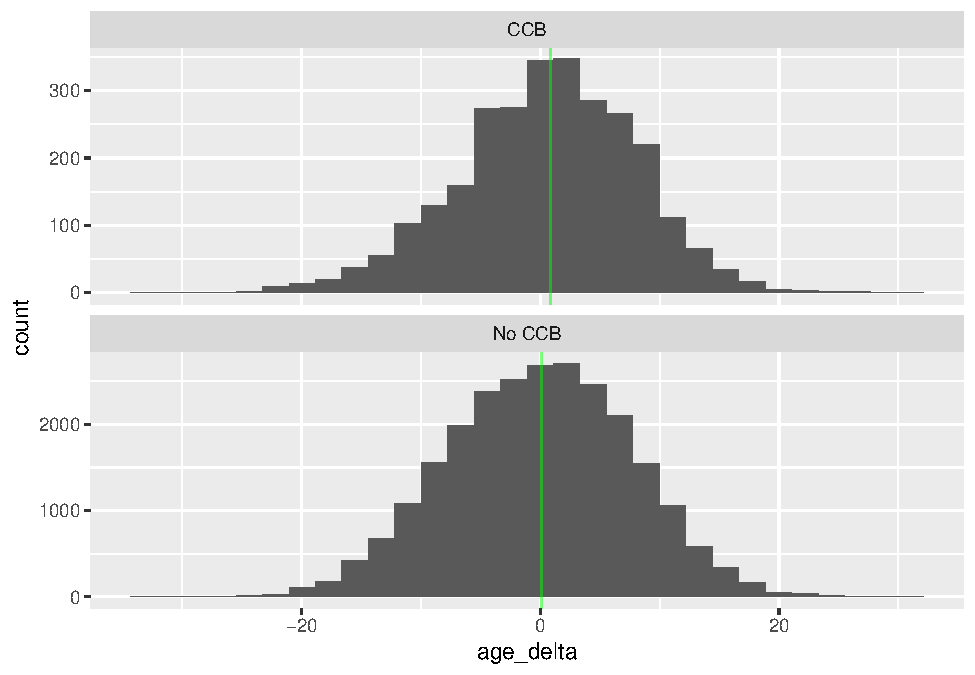
\includegraphics{../results/report_files/figure-latex/CCB-age-gap-histograms-1.pdf}

\begin{Shaded}
\begin{Highlighting}[]
\NormalTok{CCB.df }\SpecialCharTok{\%\textgreater{}\%} 
  \FunctionTok{get\_stratified\_age\_gap\_quantiles}\NormalTok{(}\StringTok{"CCB"}\NormalTok{)}
\end{Highlighting}
\end{Shaded}

\begin{verbatim}
## # A tibble: 2 x 9
##   PriorMed  `1%` `2.5%` `25%` `50%` `75%` `97.5%` `99%`     N
##   <chr>    <dbl>  <dbl> <dbl> <dbl> <dbl>   <dbl> <dbl> <int>
## 1 CCB      -18.1  -14.8 -3.98  0.88  5.83    13.9  16.3  2774
## 2 No CCB   -17.7  -15.0 -5.44  0.08  5.28    14.4  17.0 24772
\end{verbatim}

\hypertarget{lasso-6}{%
\subsubsection{Lasso}\label{lasso-6}}

\begin{Shaded}
\begin{Highlighting}[]
\NormalTok{CCB.glmnet.cv }\OtherTok{\textless{}{-}}\NormalTok{ fits.glm[[}\StringTok{"CCB"}\NormalTok{]]}
\end{Highlighting}
\end{Shaded}

\begin{Shaded}
\begin{Highlighting}[]
\FunctionTok{plot}\NormalTok{(CCB.glmnet.cv) }
\end{Highlighting}
\end{Shaded}

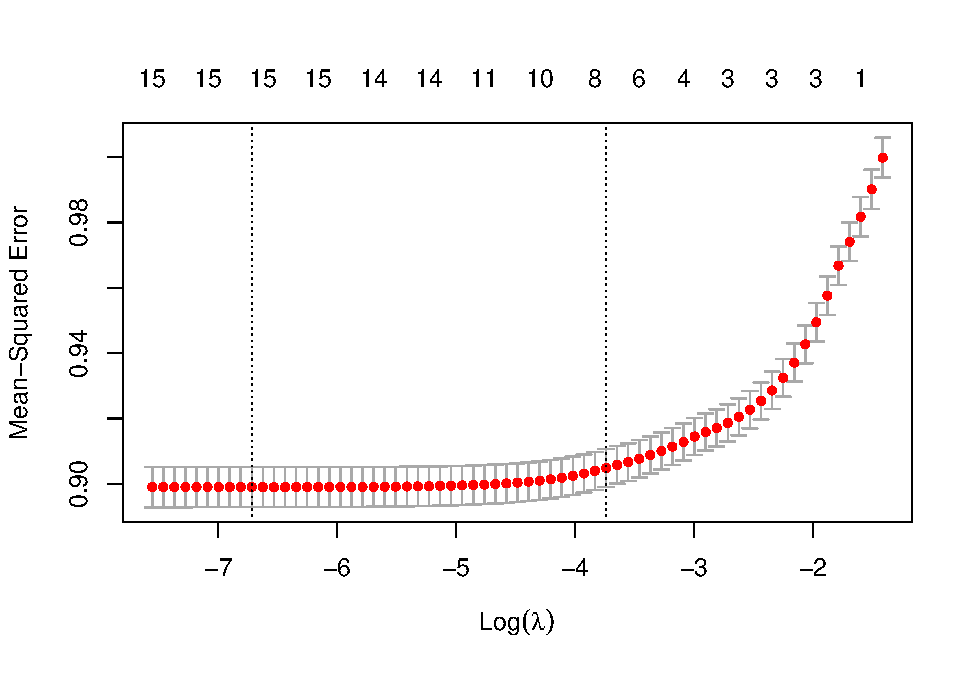
\includegraphics{../results/report_files/figure-latex/CCB-lasso-plot-1.pdf}

\begin{Shaded}
\begin{Highlighting}[]
\FunctionTok{coef}\NormalTok{(CCB.glmnet.cv, }\FunctionTok{c}\NormalTok{(CCB.glmnet.cv}\SpecialCharTok{$}\NormalTok{lambda.min,}
\NormalTok{                   CCB.glmnet.cv}\SpecialCharTok{$}\NormalTok{lambda}\FloatTok{.1}\NormalTok{se))}
\end{Highlighting}
\end{Shaded}

\begin{verbatim}
## 17 x 2 sparse Matrix of class "dgCMatrix"
##                                    s1            s2
## (Intercept)             -2.295597e-16 -1.213257e-16
## SID                      1.521459e-03  .           
## SexMale                  2.394914e-02  1.778284e-03
## Age                     -4.834152e-02 -4.750819e-03
## packyrs                  3.542791e-02  1.261464e-02
## alcoholintakegpd         3.484559e-03  .           
## PriorMed                -1.058849e-02  .           
## HypertensionTRUE         4.446964e-02  1.773942e-02
## ObesityTRUE             -1.040865e-02  .           
## `Diabetes Mellitus`TRUE  2.099499e-02  .           
## CADTRUE                  1.218835e-02  .           
## HypercholTRUE           -6.316453e-03  .           
## `Heart Failure`TRUE      .             .           
## bmi                     -8.464660e-02 -4.518251e-02
## sbp                      1.553599e-01  1.228784e-01
## dbp                      1.225816e-01  1.258928e-01
## pulse_rate               1.656166e-01  1.360434e-01
\end{verbatim}

\hypertarget{diuretics}{%
\subsection{Diuretics}\label{diuretics}}

\begin{Shaded}
\begin{Highlighting}[]
\NormalTok{diuretics.df }\OtherTok{\textless{}{-}}\NormalTok{ dfs }\SpecialCharTok{\%\textgreater{}\%} 
  \FunctionTok{filter}\NormalTok{(Drug}\SpecialCharTok{==}\StringTok{"Diuretics"}\NormalTok{) }\SpecialCharTok{\%\textgreater{}\%} 
  \FunctionTok{select}\NormalTok{(}\SpecialCharTok{{-}}\NormalTok{Drug)}
\end{Highlighting}
\end{Shaded}

\begin{Shaded}
\begin{Highlighting}[]
\NormalTok{diuretics.fits.df }\OtherTok{\textless{}{-}}\NormalTok{ fits.df }\SpecialCharTok{\%\textgreater{}\%} 
  \FunctionTok{filter}\NormalTok{(Drug}\SpecialCharTok{==}\StringTok{"Diuretics"}\NormalTok{)}
\end{Highlighting}
\end{Shaded}

\begin{Shaded}
\begin{Highlighting}[]
\FunctionTok{get\_pretty\_fit\_table}\NormalTok{(diuretics.fits.df, }\StringTok{"Diuretics"}\NormalTok{)}
\end{Highlighting}
\end{Shaded}

\begin{table}

\caption{\label{tab:diuretics-fit-table}Diuretics: Coefficients from linear models}
\centering
\begin{tabular}[t]{l|r|r|r|r|r|r|l}
\hline
term & estimate & std.error & statistic & p.value & conf.low & conf.high & Adjustment\\
\hline
(Intercept) & -20.518 & 0.517 & -39.695 & 0.000 & -21.531 & -19.505 & With SBP/DBP/HR\\
\hline
(Intercept) & -0.874 & 0.359 & -2.433 & 0.015 & -1.578 & -0.170 & Without SBP/DBP/HR\\
\hline
`Diabetes Mellitus`TRUE & 0.664 & 0.176 & 3.763 & 0.000 & 0.318 & 1.009 & With SBP/DBP/HR\\
\hline
`Diabetes Mellitus`TRUE & 0.608 & 0.183 & 3.319 & 0.001 & 0.249 & 0.968 & Without SBP/DBP/HR\\
\hline
`Heart Failure`TRUE & 0.093 & 0.371 & 0.249 & 0.803 & -0.635 & 0.820 & With SBP/DBP/HR\\
\hline
`Heart Failure`TRUE & -0.089 & 0.388 & -0.230 & 0.818 & -0.851 & 0.672 & Without SBP/DBP/HR\\
\hline
alcoholintakegpd & 0.001 & 0.003 & 0.329 & 0.742 & -0.004 & 0.006 & With SBP/DBP/HR\\
\hline
alcoholintakegpd & 0.006 & 0.003 & 2.323 & 0.020 & 0.001 & 0.011 & Without SBP/DBP/HR\\
\hline
bmi & -0.147 & 0.014 & -10.537 & 0.000 & -0.174 & -0.120 & With SBP/DBP/HR\\
\hline
bmi & 0.000 & 0.014 & -0.022 & 0.982 & -0.028 & 0.028 & Without SBP/DBP/HR\\
\hline
CADTRUE & 0.456 & 0.176 & 2.585 & 0.010 & 0.110 & 0.801 & With SBP/DBP/HR\\
\hline
CADTRUE & -0.483 & 0.183 & -2.634 & 0.008 & -0.842 & -0.123 & Without SBP/DBP/HR\\
\hline
dbp & 0.087 & 0.006 & 13.991 & 0.000 & 0.075 & 0.100 & With SBP/DBP/HR\\
\hline
HypercholTRUE & -0.142 & 0.112 & -1.269 & 0.204 & -0.361 & 0.077 & With SBP/DBP/HR\\
\hline
HypercholTRUE & -0.222 & 0.117 & -1.900 & 0.057 & -0.452 & 0.007 & Without SBP/DBP/HR\\
\hline
HypertensionTRUE & 0.643 & 0.105 & 6.133 & 0.000 & 0.437 & 0.848 & With SBP/DBP/HR\\
\hline
HypertensionTRUE & 1.849 & 0.106 & 17.403 & 0.000 & 1.641 & 2.058 & Without SBP/DBP/HR\\
\hline
ObesityTRUE & -0.257 & 0.148 & -1.733 & 0.083 & -0.547 & 0.034 & With SBP/DBP/HR\\
\hline
ObesityTRUE & -0.738 & 0.155 & -4.768 & 0.000 & -1.041 & -0.435 & Without SBP/DBP/HR\\
\hline
packyrs & 0.023 & 0.004 & 6.045 & 0.000 & 0.015 & 0.030 & With SBP/DBP/HR\\
\hline
packyrs & 0.022 & 0.004 & 5.468 & 0.000 & 0.014 & 0.029 & Without SBP/DBP/HR\\
\hline
poly(Age, 2)1 & -68.955 & 8.366 & -8.242 & 0.000 & -85.352 & -52.557 & With SBP/DBP/HR\\
\hline
poly(Age, 2)1 & -24.164 & 7.944 & -3.042 & 0.002 & -39.734 & -8.595 & Without SBP/DBP/HR\\
\hline
poly(Age, 2)2 & -106.461 & 7.247 & -14.691 & 0.000 & -120.666 & -92.257 & With SBP/DBP/HR\\
\hline
poly(Age, 2)2 & -113.260 & 7.563 & -14.975 & 0.000 & -128.084 & -98.436 & Without SBP/DBP/HR\\
\hline
PriorMed & 0.113 & 0.221 & 0.511 & 0.610 & -0.320 & 0.545 & With SBP/DBP/HR\\
\hline
PriorMed & -0.289 & 0.231 & -1.254 & 0.210 & -0.741 & 0.163 & Without SBP/DBP/HR\\
\hline
pulse\_rate & 0.110 & 0.004 & 27.846 & 0.000 & 0.103 & 0.118 & With SBP/DBP/HR\\
\hline
sbp & 0.067 & 0.003 & 19.637 & 0.000 & 0.061 & 0.074 & With SBP/DBP/HR\\
\hline
SexMale & 0.452 & 0.095 & 4.774 & 0.000 & 0.266 & 0.638 & With SBP/DBP/HR\\
\hline
SexMale & 0.517 & 0.096 & 5.381 & 0.000 & 0.329 & 0.705 & Without SBP/DBP/HR\\
\hline
\end{tabular}
\end{table}

\begin{Shaded}
\begin{Highlighting}[]
\FunctionTok{get\_pretty\_fit\_forest\_plot}\NormalTok{(diuretics.fits.df) }\OtherTok{{-}\textgreater{}}\NormalTok{p}
\NormalTok{p}
\end{Highlighting}
\end{Shaded}

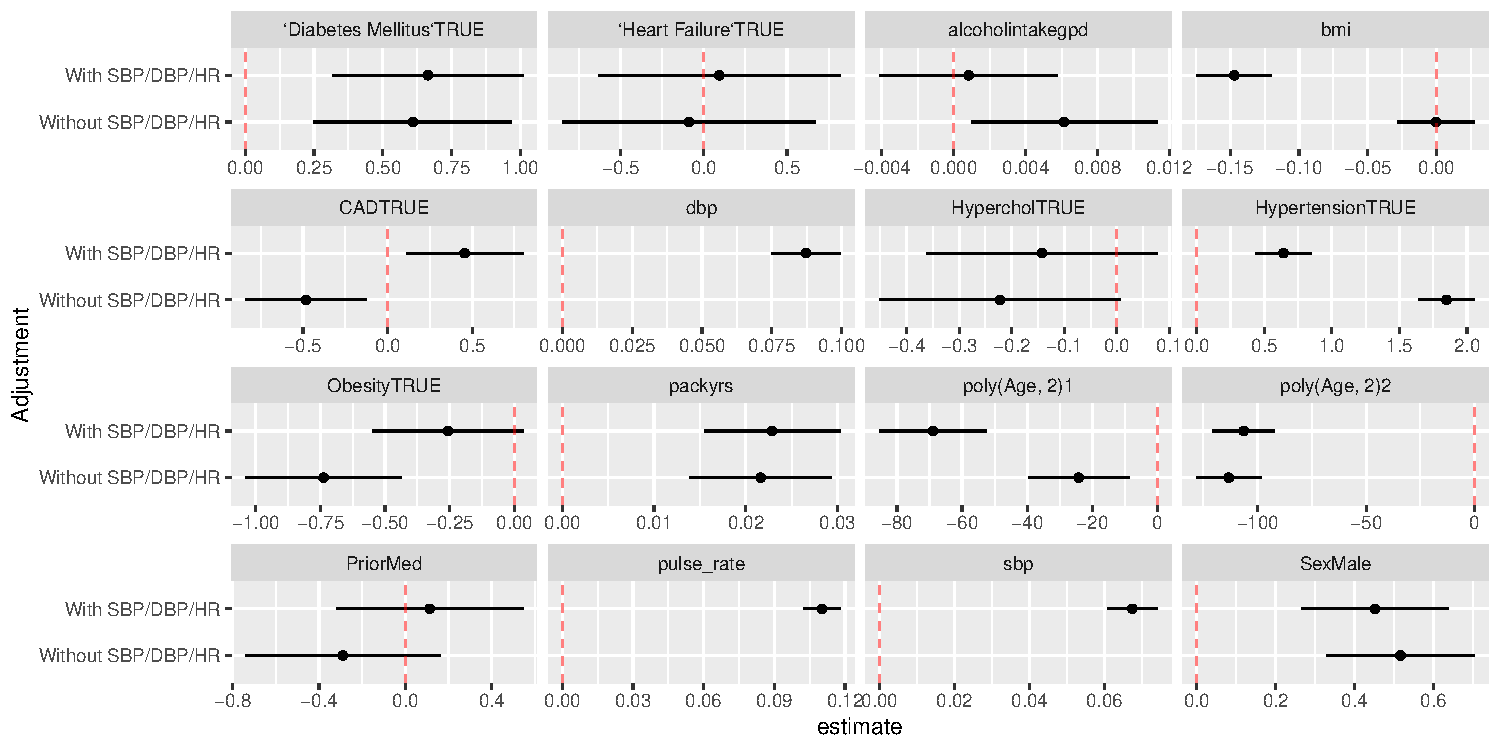
\includegraphics{../results/report_files/figure-latex/diuretics-fit-forest-1.pdf}

\begin{Shaded}
\begin{Highlighting}[]
\NormalTok{diuretics.fits.df }\SpecialCharTok{\%\textgreater{}\%} 
\NormalTok{  get\_fit\_glance}
\end{Highlighting}
\end{Shaded}

\begin{verbatim}
## # A tibble: 2 x 5
##   AdditionalMarkers     N fracPriorMed adj.r.squared r.squared
##   <lgl>             <dbl>        <dbl>         <dbl>     <dbl>
## 1 FALSE             27546        0.045         0.024     0.024
## 2 TRUE              27546        0.045         0.108     0.109
\end{verbatim}

\begin{Shaded}
\begin{Highlighting}[]
\FunctionTok{generate\_table.self.reported}\NormalTok{(diuretics.df, }\StringTok{"diuretics"}\NormalTok{)}
\end{Highlighting}
\end{Shaded}

\begin{verbatim}
## Table printed with `knitr::kable()`, not {gt}. Learn why at
## https://www.danieldsjoberg.com/gtsummary/articles/rmarkdown.html
## To suppress this message, include `message = FALSE` in code chunk header.
\end{verbatim}

\begin{tabular}{l|c|c|c}
\hline
**Characteristic** & **diuretics**, N = 1,230 & **No diuretics**, N = 26,316 & **p-value**\\
\hline
Cardiac Age gap & 1.0 (-3.9, 5.8) & 0.1 (-5.4, 5.3) & <0.001\\
\hline
Sex &  &  & 0.6\\
\hline
Female & 608 (49\%) & 13,229 (50\%) & \\
\hline
Male & 622 (51\%) & 13,087 (50\%) & \\
\hline
Age & 68 (63, 72) & 64 (58, 70) & <0.001\\
\hline
Packs year of smoking & 0 (0, 6) & 0 (0, 3) & 0.019\\
\hline
Alcohol is g/day consumed & 3 (0, 14) & 4 (0, 15) & 0.003\\
\hline
Hypertension & 1,148 (93\%) & 8,050 (31\%) & <0.001\\
\hline
Obesity & 447 (36\%) & 5,228 (20\%) & <0.001\\
\hline
Diabetes Mellitus & 202 (16\%) & 1,781 (6.8\%) & <0.001\\
\hline
Coronary Artery Disease & 202 (16\%) & 1,906 (7.2\%) & <0.001\\
\hline
Hypercholesterolemia & 546 (44\%) & 5,745 (22\%) & <0.001\\
\hline
Heart Failure & 83 (6.7\%) & 329 (1.3\%) & <0.001\\
\hline
dbp & 80 (73, 86) & 78 (72, 85) & <0.001\\
\hline
sbp & 143 (131, 155) & 138 (126, 150) & <0.001\\
\hline
pulse\_rate & 70 (62, 79) & 68 (61, 76) & <0.001\\
\hline
bmi & 28.5 (25.7, 31.8) & 26.2 (23.7, 29.2) & <0.001\\
\hline
\end{tabular}

\begin{Shaded}
\begin{Highlighting}[]
\NormalTok{diuretics.df }\SpecialCharTok{\%\textgreater{}\%} 
  \FunctionTok{get\_stratified\_age\_gap\_histogram}\NormalTok{(}\StringTok{"Diuretics"}\NormalTok{)}
\end{Highlighting}
\end{Shaded}

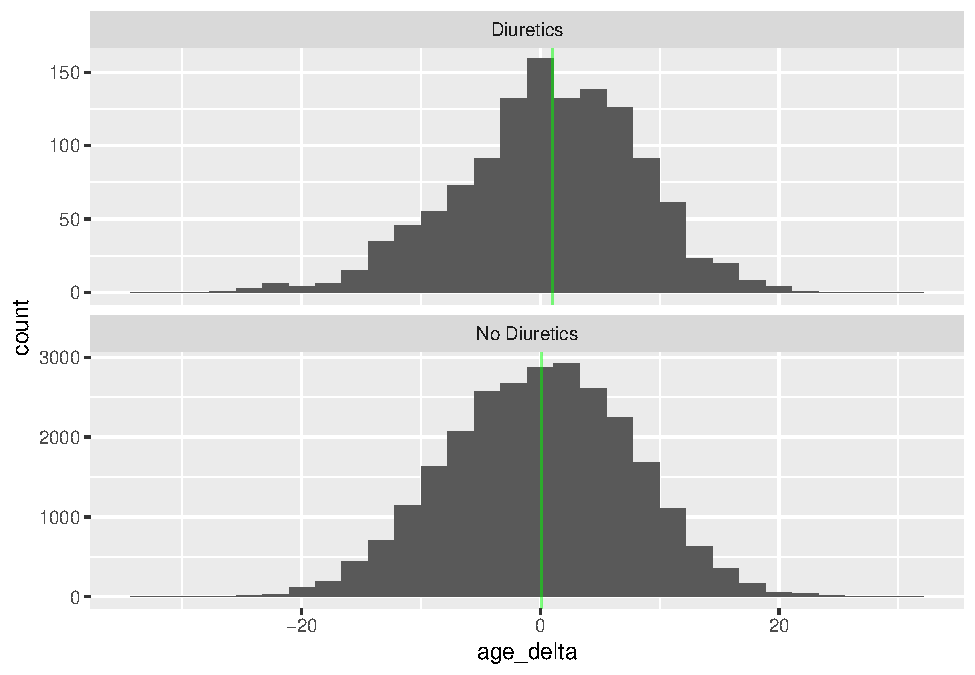
\includegraphics{../results/report_files/figure-latex/diuretics-age-gap-histograms-1.pdf}

\begin{Shaded}
\begin{Highlighting}[]
\NormalTok{diuretics.df }\SpecialCharTok{\%\textgreater{}\%} 
 \FunctionTok{get\_stratified\_age\_gap\_quantiles}\NormalTok{(}\StringTok{"Diuretics"}\NormalTok{)}
\end{Highlighting}
\end{Shaded}

\begin{verbatim}
## # A tibble: 2 x 9
##   PriorMed      `1%` `2.5%` `25%` `50%` `75%` `97.5%` `99%`     N
##   <chr>        <dbl>  <dbl> <dbl> <dbl> <dbl>   <dbl> <dbl> <int>
## 1 Diuretics    -20.4  -14.8 -3.94  0.99  5.79    14.5  16.5  1230
## 2 No Diuretics -17.7  -15.0 -5.35  0.13  5.3     14.4  17.0 26316
\end{verbatim}

\hypertarget{lasso-7}{%
\subsubsection{Lasso}\label{lasso-7}}

\begin{Shaded}
\begin{Highlighting}[]
\NormalTok{diuretics.glmnet.cv }\OtherTok{\textless{}{-}}\NormalTok{ fits.glm[[}\StringTok{"Diuretics"}\NormalTok{]]}
\end{Highlighting}
\end{Shaded}

\begin{Shaded}
\begin{Highlighting}[]
\FunctionTok{plot}\NormalTok{(diuretics.glmnet.cv) }
\end{Highlighting}
\end{Shaded}

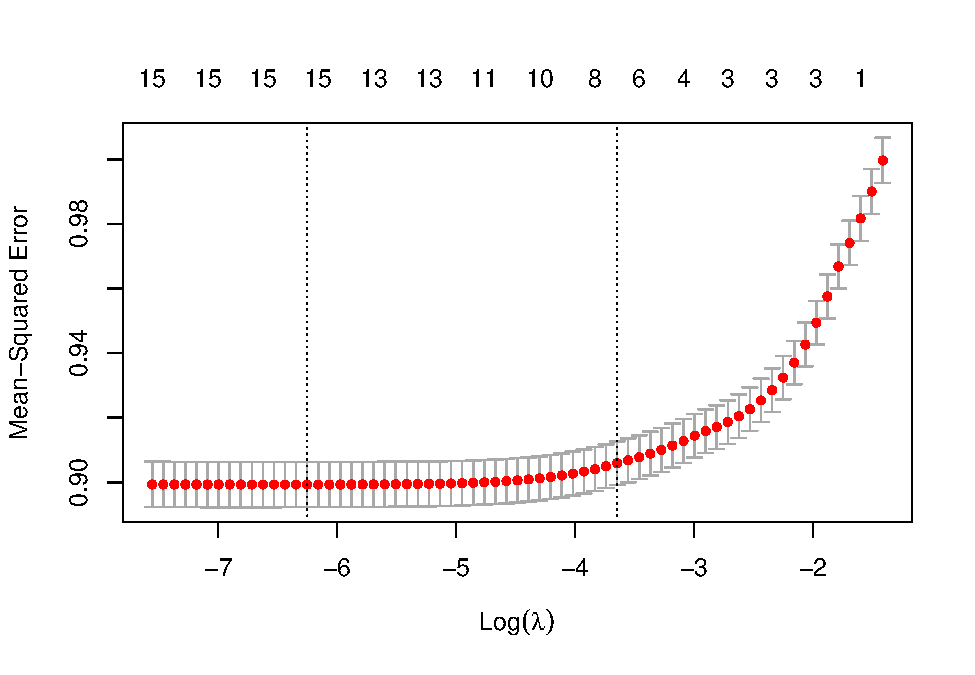
\includegraphics{../results/report_files/figure-latex/diuretics-lasso-plot-1.pdf}

\begin{Shaded}
\begin{Highlighting}[]
\FunctionTok{coef}\NormalTok{(diuretics.glmnet.cv, }\FunctionTok{c}\NormalTok{(diuretics.glmnet.cv}\SpecialCharTok{$}\NormalTok{lambda.min,}
\NormalTok{                   diuretics.glmnet.cv}\SpecialCharTok{$}\NormalTok{lambda}\FloatTok{.1}\NormalTok{se))}
\end{Highlighting}
\end{Shaded}

\begin{verbatim}
## 17 x 2 sparse Matrix of class "dgCMatrix"
##                                    s1            s2
## (Intercept)             -2.278847e-16 -1.144220e-16
## SID                      8.914631e-04  .           
## SexMale                  2.281645e-02  .           
## Age                     -4.776635e-02 -3.901188e-04
## packyrs                  3.477911e-02  1.000863e-02
## alcoholintakegpd         2.893804e-03  .           
## PriorMed                 1.147081e-03  .           
## HypertensionTRUE         3.879576e-02  1.517539e-02
## ObesityTRUE             -9.901109e-03  .           
## `Diabetes Mellitus`TRUE  2.008850e-02  .           
## CADTRUE                  1.145429e-02  .           
## HypercholTRUE           -5.394407e-03  .           
## `Heart Failure`TRUE      .             .           
## bmi                     -8.377949e-02 -4.076007e-02
## sbp                      1.545863e-01  1.195392e-01
## dbp                      1.232900e-01  1.262449e-01
## pulse_rate               1.643293e-01  1.331395e-01
\end{verbatim}

\hypertarget{self-reported-drugs-used}{%
\subsection{Self-reported drugs used}\label{self-reported-drugs-used}}

\begin{Shaded}
\begin{Highlighting}[]
\FunctionTok{read\_csv}\NormalTok{(}\StringTok{"../data/Derived/self\_reported\_drugs\_used.csv"}\NormalTok{)}
\end{Highlighting}
\end{Shaded}

\begin{verbatim}
## Rows: 79 Columns: 2
## -- Column specification ------------------------------------------------------------------------------
## Delimiter: ","
## chr (2): meaning, Drug
## 
## i Use `spec()` to retrieve the full column specification for this data.
## i Specify the column types or set `show_col_types = FALSE` to quiet this message.
\end{verbatim}

\begin{verbatim}
## # A tibble: 79 x 2
##    meaning                                                    Drug     
##    <chr>                                                      <chr>    
##  1 amiloride                                                  Diuretics
##  2 atenolol+bendroflumethiazide                               Diuretics
##  3 bendroflumethiazide                                        Diuretics
##  4 bendroflumethiazide+potassium 2.5mg/7.7mmol m/r tablet     Diuretics
##  5 bisoprolol fumarate+hydrochlorothiazide 10mg/6.25mg tablet Diuretics
##  6 bumetanide                                                 Diuretics
##  7 captopril+hydrochlorothiazide 25mg/12.5mg tablet           Diuretics
##  8 cyclopenthiazide                                           Diuretics
##  9 diltiazem hcl+hydrochlorothiazide 150mg/12.5mg m/r capsule Diuretics
## 10 enalapril maleate+hydrochlorothiazide 20mg/12.5mg tablet   Diuretics
## # ... with 69 more rows
## # i Use `print(n = ...)` to see more rows
\end{verbatim}

\end{document}
